% %%%%%%%%%%%%%%%%%%%%%%%%%%%%%%%%%%%%%%%%%%%%%%%%%%%%%%%%%
% Template created by Yang Ma, April-2022.
% Last update: April-2022.
% Contact: mayangluon@pitt.edu
%
% DISCLAIMER: This is not an official PITTPACC template.
% %%%%%%%%%%%%%%%%%%%%%%%%%%%%%%%%%%%%%%%%%%%%%%%%%%%%%%%%%

% ---------------------------------------
\documentclass[aspectratio=169]{beamer}
\usepackage{PITTtheme}
% ---------------------------------------

%% ===========================================
%% ===========================================
\title[YM PhD. defense]{\huge Electroweak and Higgs physics at high energies}
\author{Yang Ma}
\institute{Department of Physics and Astronomy \\ University of Pittsburgh}
\date{April 19, 2022}

%% ===========================================
%% ===========================================
% Don't change this part.
\begin{document}

% Water marks 
\newwatermark*[pages=6,scale=0.3,xpos=21,ypos=-14]{\hspace{8mm}\textcolor{PittRoyal}{ $\gamma\gamma$ collision}}
\newwatermark*[pages=6,scale=0.3,xpos=23,ypos=-30]{\hspace{8mm}\textcolor{PittRoyal}{ISR}}

\newwatermark*[pages=8,scale=1,xpos=48,ypos=28]{

\includegraphics[width=0.1\textwidth]{figs/IMCC-Logo.png}}

\newwatermark*[pages=28,color=green,scale=0.18,xpos=40,ypos=-32]{
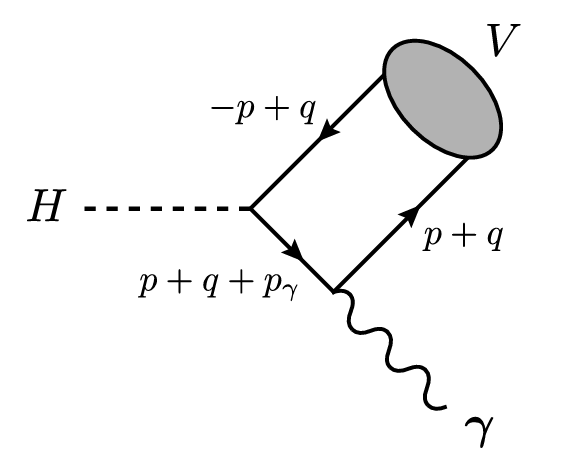
\includegraphics{figs/HJpsigm.png}}

\newwatermark*[pages=37,scale=0.8,xpos=45,ypos=-39]{

\includegraphics[width=0.1\textwidth]{Logo/Seal_of_the_University_of_Bologna.pdf}}
\newwatermark*[pages=37,scale=1,xpos=30,ypos=-37]{

\includegraphics[width=0.1\textwidth]{Logo/NEW_LOGO_BOLOGNA.png}}

%% ===========================================
%% ===========================================
% Title page 
\begin{frame}[plain]
\Background
    \titlepage
	% \vspace{-22mm}\hspace{90mm}
\includegraphics[height=1.8cm]{Logo/pittpacc_logo.png}
\end{frame}

%% ===========================================
%% ===========================================
% Uncomment these lines for an automatically generated outline.
% \begin{frame}{Outline}
% % \Background
% \setcounter{page}{0}
% % \thispagestyle{empty}
% \tableofcontents
% \end{frame}


%% ===========================================
%% ===========================================
%	PRESENTATION SLIDES
%% ===========================================
%% ===========================================

%% ===========================================
%% ===========================================
\section[Publications \& Presentations]{Achievements during the Ph.D. career} % Sections can be created in order to organize your presentation into discrete blocks, all sections and subsections are automatically printed in the table of contents as an overview of the talk
%% ===========================================
%% ===========================================

% \subsection{Subsection Example} % A subsection can be created just before a set of slides with a common theme to further break down your presentation into chunks
\subsection{Publications \& Presentations}
%%%%%%%%%%%%%%%%%%%%%%%%%%%%%%%%%%%%%%%%%%%%
% Publication list
%%%%%%%%%%%%%%%%%%%%%%%%%%%%%%%%%%%%%%%%%%%%
\begin{frame}
	\frametitle{Publications}
	{\tiny
	\nocite{*}                   %this uses *everything* in the .bib file
	\bibliography{ref.bib}        %or whatever your .bib file is
	\bibliographystyle{JHEP}   %if you use utphys.bst
	}
\end{frame}
%%%%%%%%%%%%%%%%%%%%%%%%%%%%%%%%%%%%%%%%%%%%
% Presentation list
%%%%%%%%%%%%%%%%%%%%%%%%%%%%%%%%%%%%%%%%%%%%
\begin{frame}
	\frametitle{Presentations}
	\begin{exampleblock}{Seminar and Colloquium (Invited)}
		\begin{itemize}
			\item {\it Higgs decay to charmonia and the Charm Yukawa coupling}
			\hspace{8mm}~\textcolor{green}{\small UCLA, (scheduled) May 2022}
			\item {\it Multi-boson production and the muon Yukawa coupling}\hspace{13mm}~\textcolor{green}{\small Univ. of Utah, Oct. 2021}
			\item {\it Parton contents of a lepton at high energies}
			\hspace{30mm}~\textcolor{green}{\small Carleton Univ. May 2021}
			\item {\it The partonic picture at high-energy lepton colliders}
			\hspace{19mm}~~\textcolor{green}{\small SLAC, Apr. 2021}
			\item {\it Parton contents of a lepton at high energies}
			\hspace{30mm}~~\textcolor{green}{\small Oklahoma State Univ. Apr. 2021}
			\item {\it High energy lepton collisions and electroweak PDFs}
			\hspace{19mm}~~\textcolor{green}{\small Carleton Univ. Oct. 2020}
		\end{itemize}
	\end{exampleblock}
	\begin{block}{Talks given at conferences}
		\begin{itemize}
			\item 2022: {\it APS April Meeting 2022}
			\item 2021: {\it Higgs 2021, SUSY 2021, EPS-HEP 2021, DPF 2021, Pheno 2021, PPC 2021, etc.}
			\item 2020: {\it Pheno 2020}
		\end{itemize}
	\end{block}
\end{frame}


\begin{frame}
	\frametitle{Outline}
	\vspace{-3mm}
	\begin{block}{The partonic picture of high-energy colliders}
		\begin{itemize}
			\item Parton Distribution Functions (PDF)
			\item Future high-energy lepton colliders
			\item Electroweak PDF (EW PDF) and its evolution
			\item The Standard Model expectation for future high-energy lepton colliders
		\end{itemize}
	\end{block}
	\vspace{-3mm}
	\begin{block}{Multi-boson productions at a high-energy muon collider and the Muon-Higgs coupling}
		\begin{itemize}
			\item Multi-boson physics at future high-energy lepton collider
			\item Muon-Higgs coupling
		\end{itemize}
	\end{block}
	\vspace{-3mm}
	\begin{block}{Higgs decay to charmonia and the Charm Yukawa}
		\begin{itemize}
			\item Non-relatisvistic Quantum chromodynamics (NRQCD) calculation formalism
			\item Probe the Charm-Higgs coupling
		\end{itemize}
	\end{block}
	\vspace{-2mm}
	\textcolor{PittRoyal}{Conclusion}
\end{frame}

%% ===========================================
%% The presentation starts
%% ===========================================
\section{The partonic picture of high-energy colliders}
\subsection{Parton Distribution Functions (PDF)}

%%%%%%%%%%%%%%%%%%%%%%%%%%%%%%%%%%%%%%%%%%%%
% Backaground: PDF 
%%%%%%%%%%%%%%%%%%%%%%%%%%%%%%%%%%%%%%%%%%%%
\begin{frame}{Hadron colliders and the Parton Distribution Function (PDF) }
	\vspace{2mm}  \textcolor{PittRoyal}{\bf $\bullet$ Recall the hadron colliders: the ${\rm Sp{\bar p}S}$, the Tevatron or the LHC}
	\begin{columns}
		\begin{column}{0.6\textwidth}
			\begin{center}
				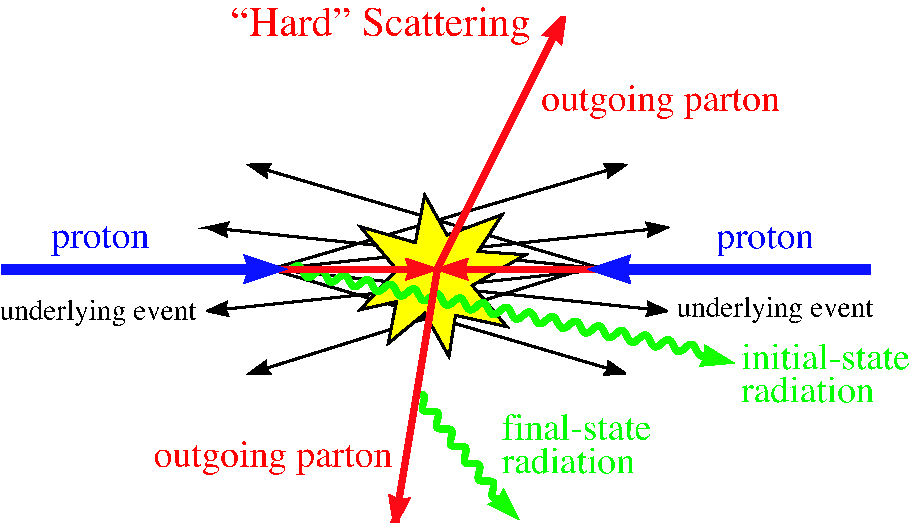
\includegraphics[width=0.8\textwidth,height=4cm]{figs/hardscattering1-hepph}
			\end{center}	
		\end{column}
		\begin{column}{0.4\textwidth}
			\begin{itemize}
				\item {\bf Hadrons are composite}\\ $a$, $b$ are the ``partons'' from the beam particles $A$ and $B$.
				\item {\bf PDFs}\\
				$f_{a/A}$, $f_{b/B}$ are the probabilities to find a parton $a$ ($b$) from the beam particle $A$ ($B$) with a momentum fraction $x_a$ ($x_b$).
			\end{itemize}
		\end{column}
	\end{columns}

	\textcolor{PittRoyal}{\bf$\bullet$ Factorization formalism : PDFs $\otimes$ partonic cross sections}
	\begin{eqnarray}
		\sigma(AB\to X)=\sum_{a,b} \int\dd x_{a}\dd x_{b} \textcolor{red}{f_{a/A}(x_{a},Q) f_{b/B}(x_{b},Q)} \textcolor{blue}{ \hat{\sigma}(ab\to X)}\nonumber
	\end{eqnarray}
\end{frame}

%%%%%%%%%%%%%%%%%%%%%%%%%%%%%%%%%%%%%%%%%%%%
% Backaground: EPA
%%%%%%%%%%%%%%%%%%%%%%%%%%%%%%%%%%%%%%%%%%%%
\begin{frame}{Lepton colliders and Equivalent Photon Appromation (EPA)}
	\vspace{1mm} \textcolor{PittRoyal}{\bf $\bullet$ Leptons are elementary particles}{\bf ~~$\Rightarrow$ ``Equivalent photon approximation (EPA)''}

		\begin{columns}
			\begin{column}{0.64\textwidth}
				\begin{itemize}
					\item  Treat photon as a parton constituent in the electron  %\bib{ C. F. von Weizsacker, Z. Phys. 88, 612 (1934)} \bib{E. J. Williams, Phys. Rev. 45, 729 (1934)}
					\begin{small}
					\begin{eqnarray}
						\sigma(\ell^- +a \to \ell^- +X) =\int \dd x \,f_{\gamma/\ell} {\hat \sigma}(\gamma a\to X) \nonumber \\
						f_{\gamma/\ell,\textrm{EPA}}(x_\gamma,Q^2)=\frac{\alpha}{2\pi}\frac{1+(1-x_\gamma)^2}{x_\gamma}\ln{Q^2 \over m_\ell^2}\nonumber 
					\end{eqnarray}
					\end{small}
				\item At lepton colliders
				\begin{small}
				\begin{eqnarray}
					\sigma(\ell^+\ell^- \rightarrow F + X) = \int_{\tau_{0}}^{1} d\tau  \sum_{ij}\frac{d\mathcal{L}_{ij}}{d\tau}\  \hat{\sigma}(ij\rightarrow F), ~\tau = \hat s/s\nonumber\\
					{ d\mathcal{L}_{ij} \over {d\tau} } = \frac{1}{1+\delta_{ij}}  \int^{1}_{\tau} \frac{d\xi}{\xi} \left[ f_{i}(\xi, Q^{2})f_{j}\left(\frac{\tau}{\xi},Q^{2} \right) + (i \leftrightarrow j) \right] \nonumber
				\end{eqnarray}
			\end{small}
			\end{itemize}
			\end{column}
			\begin{column}{0.38\textwidth}
				\begin{center}
				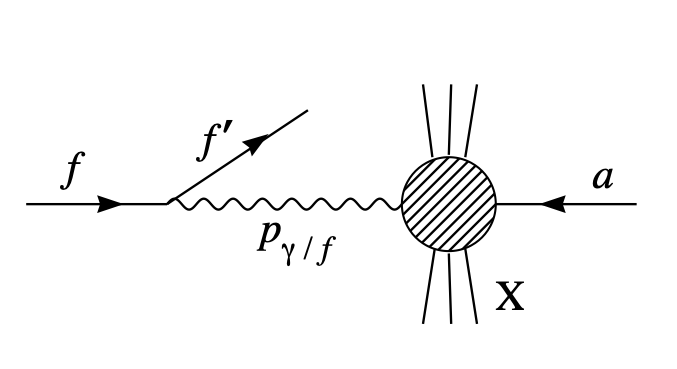
\includegraphics[width=0.9\textwidth,height=2.5cm]{figs/EPA.png}
				\end{center}
				\vspace{-8mm}
				\bib{ C. F. von Weizsacker, Z. Phys. 88, 612 (1934)}\\ \bib{E. J. Williams, Phys. Rev. 45, 729 (1934)}
				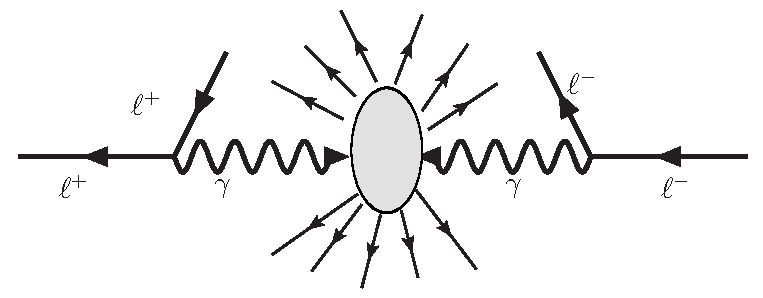
\includegraphics[width=0.8\textwidth]{figs/EPA_collision2.pdf}
				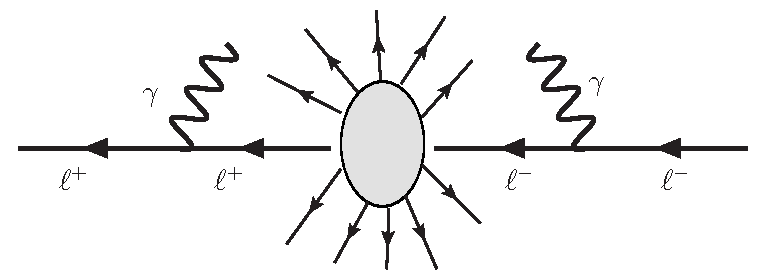
\includegraphics[width=0.8\textwidth]{figs/ISR_collision2.pdf}
			\end{column}
			\end{columns}
\end{frame}


\subsection{Future high-energy lepton colliders}
%%%%%%%%%%%%%%%%%%%%%%%%%%%%%%%%%%%%%%%%%%%%
% MuC: why
%%%%%%%%%%%%%%%%%%%%%%%%%%%%%%%%%%%%%%%%%%%%
\begin{frame}{A possible high-energy lepton collider in the future}
	\textcolor{PittRoyal}{{\bf Why lepton colliders?}}
	\begin{itemize}
	\item \textcolor{PittRoyal}{{\bf Leptons} are the ideal probes of short-distance physics}
	\begin{itemize}
		\item Cleaner background comparing to hadron colliders
		\item The collision particles can carry the full machine energy
	\end{itemize}
	\item \textcolor{PittRoyal}{{\bf ee colliders}}
	\begin{itemize}
		\item A glorious past: discovery of charm, $\tau$, and gluon 
		\item Important future: Precision EW constraints on BSM physicss, Higgs physics
	\end{itemize}
	\item \textcolor{PittRoyal}{{\bf Muon colliders}}
	\begin{itemize}
		\item \textcolor{PittRoyal}{A $s$-channel Higgs factory}: Higgs production enhanced by $m_\mu^2/m_e^2\sim 40000$
		\begin{itemize}
			\item Direct measurements on $y_\mu$ and $\Gamma_H$
		\end{itemize}
		\item \textcolor{PittRoyal}{Multi-TeV muon colliders}: Less radiations than electron
		\begin{itemize}
			\item Center of mass energy $3 -15$ TeV and the more speculative $E_{\rm cm}=30$ TeV
			\item New particle mass coverage $M \sim (0.5 - 1 ) E_{\rm cm}$
			\item Great accuracies for $WWH$, $WWHH$, $H^3$, $H^4$
			\item $\cdots$
		\end{itemize}
	\end{itemize}
	\end{itemize}
\end{frame}

%%%%%%%%%%%%%%%%%%%%%%%%%%%%%%%%%%%%%%%%%%%%
% MuC: size
%%%%%%%%%%%%%%%%%%%%%%%%%%%%%%%%%%%%%%%%%%%%
\begin{frame}{The dream machine: A possible high-energy muon collider}
	\vspace{2mm}\hspace{3mm}\textcolor{PittRoyal}{\bf $\bullet$ Size and Benchmarks}\\
	\begin{center}
	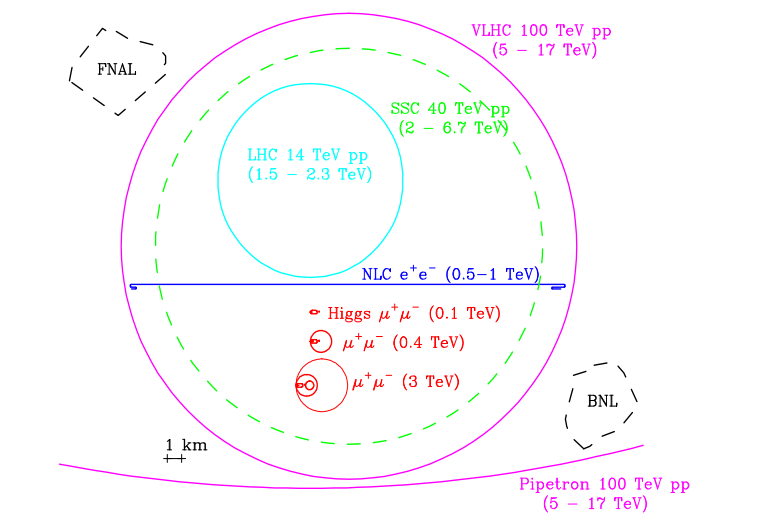
\includegraphics[width=0.4\textwidth]{figs/muCsize.png}\\
	\hspace{40mm}\bib{Ankenbrandt et al. arXiv:physics/9901022}
	\end{center}
	\hspace{5mm}\small{\textcolor{PittRoyal}{\bf $\bullet$ Luminosity}: ${\cal L} = (E_{\rm cm}/10~{\rm TeV})^2 \times 10 {\rm ab}^{-1}$}
	\begin{center}
	\includegraphics[width=0.5\textwidth]{figs/muCLumi.png}\\
	\hspace{40mm}\bib{arXiv: 2103.14043}
	\end{center}
\end{frame}


%%%%%%%%%%%%%%%%%%%%%%%%%%%%%%%%%%%%%%%%%%%%
% EPA plot
%%%%%%%%%%%%%%%%%%%%%%%%%%%%%%%%%%%%%%%%%%%%
\begin{frame}{A high-energy muon collider at first glance}
	\vspace{-2mm}\textcolor{PittRoyal}{\bf What do people expect from a high-energy lepton (muon) collider?}\\
		\vspace*{2mm}
		\begin{columns}
		\begin{column}{0.5\textwidth}
		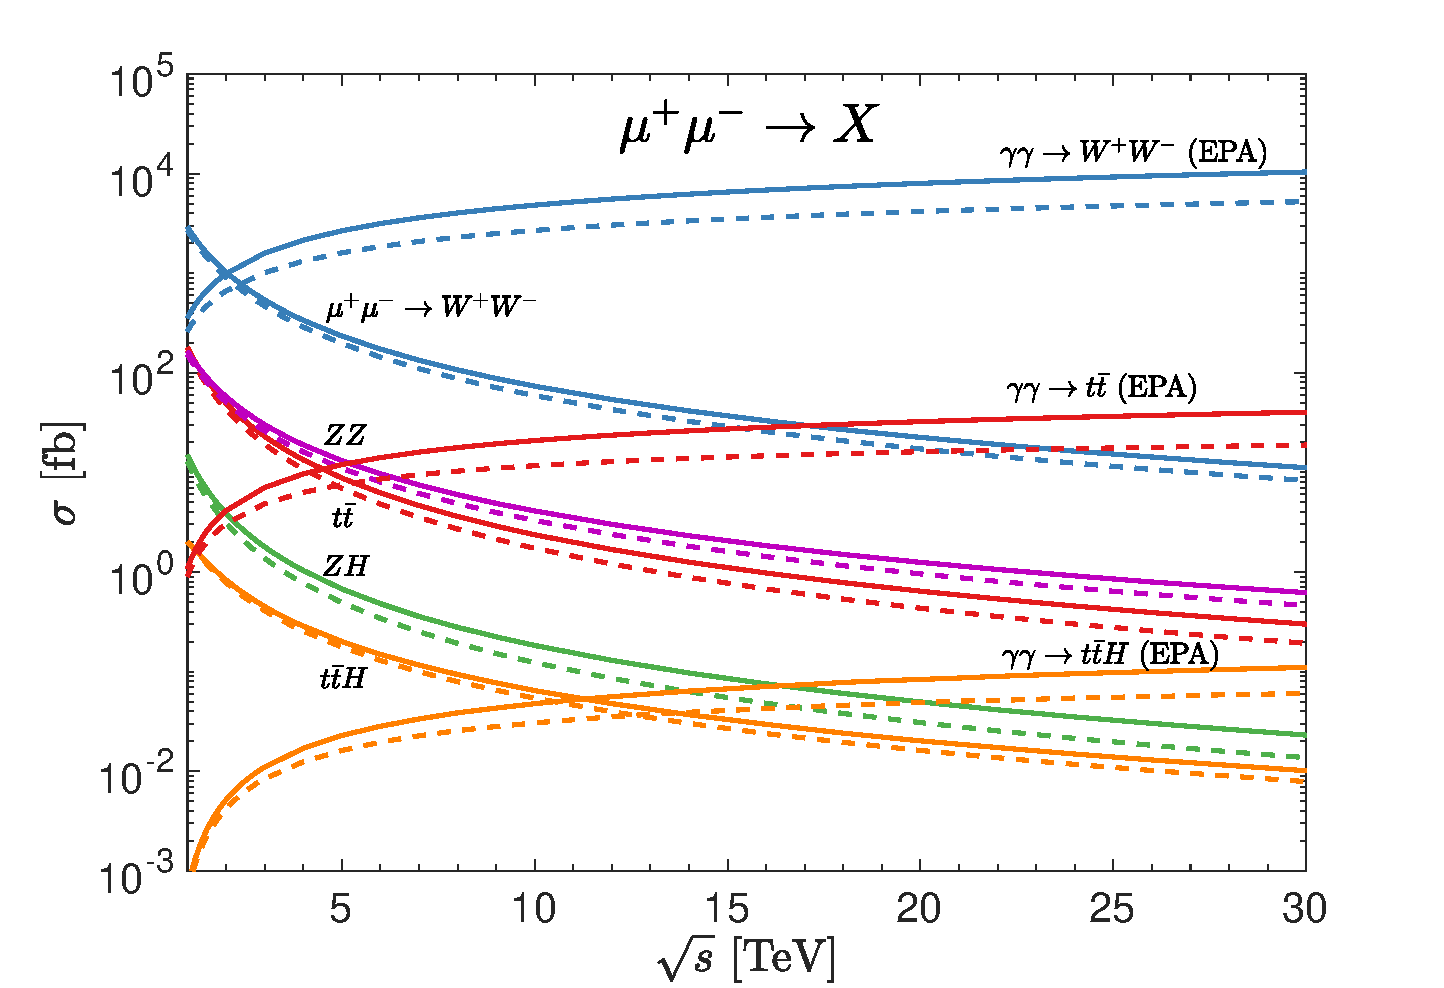
\includegraphics[width=1\textwidth]{figs/sigma_FO2}
		\vspace{3pt}\hspace{40mm}\bib{T. Han, YM, K.Xie 2007.14300}
		\end{column}
		\begin{column}{0.5\textwidth}
			\textcolor{black}{\bf Some ``commonsense'':}
			\begin{itemize}
				\item The annihilations decrease as $1/s$.
				\item ISR needs to be considered, which can give over $10\%$ enhancement.
				\item The fusions increase as $\ln^p(s)$, which take over at high energies.
				\item The large collinear logarithm $\ln(s/m_\ell^2)$ needs to be resummed, set $Q={\sqrt {\hat s}}/2$,
				\item $\gamma\gamma \to W^+W^-$ production has the largest cross section.
			\end{itemize}
		\end{column}
	\end{columns}
\end{frame}

%%%%%%%%%%%%%%%%%%%%%%%%%%%%%%%%%%%%%%%%%%%%
% Traditional Background
%%%%%%%%%%%%%%%%%%%%%%%%%%%%%%%%%%%%%%%%%%%%
\begin{frame}
	% \frametitle{A high-energy lepton collider at first glance (II)}
	\textcolor{PittRoyal}{\bf What are the dominant processes at a high-energy lepton collider? }
	\begin{itemize}
		\item Leading-order: $\ell^+\ell^- \to \ell^+\ell^-,\,\tau^+\tau^-,\,q{\bar q},\, W^+W^-$, and $\gamma \ell \to \gamma \ell$
		\item $\gamma \gamma$ scatterings: $\gamma\gamma \to \tau^+\tau^-,\,q{\bar q},\, W^+W^-$
	\end{itemize}
	\textcolor{PittRoyal}{\bf Need some cuts: }
	\begin{itemize}
		\item Detector angle \& Threshold: $\theta_{\rm cut}=5^\circ\,(10^\circ)\Longleftrightarrow |\eta|<3.13 (2.44)$, $m_{ij}>20$ GeV
		\item To separate from the nonperturbative hadronic production: $p_T>\left(4+\frac{\sqrt s}{3 \,{\rm TeV}}\right)\,{\rm GeV}$\\
		\bib{ Drees and Godbole, PRL 67, 1189; Chen, Barklow, and Peskin, hep-ph/9305247;T. Barklow, etal, LCD-2011-020}
	\end{itemize}
	\begin{columns}
	\begin{column}{0.5\textwidth}
	\hspace{10mm}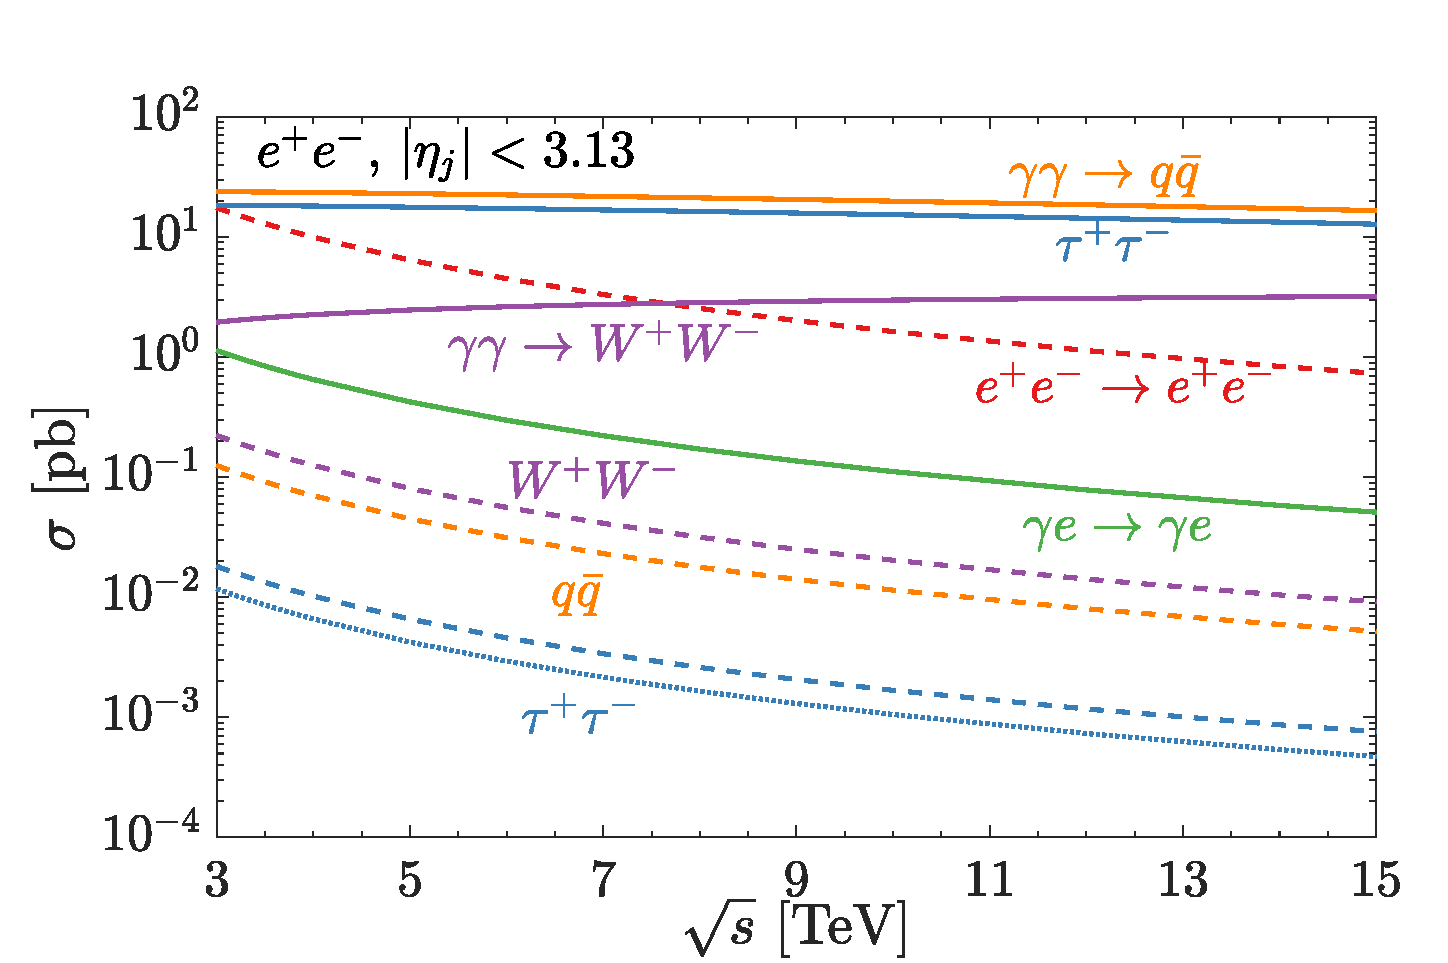
\includegraphics[width=0.8\textwidth]{figs/sigma_eeCollider_c5_3pt_s20}
	\end{column}
	\begin{column}{0.5\textwidth}
		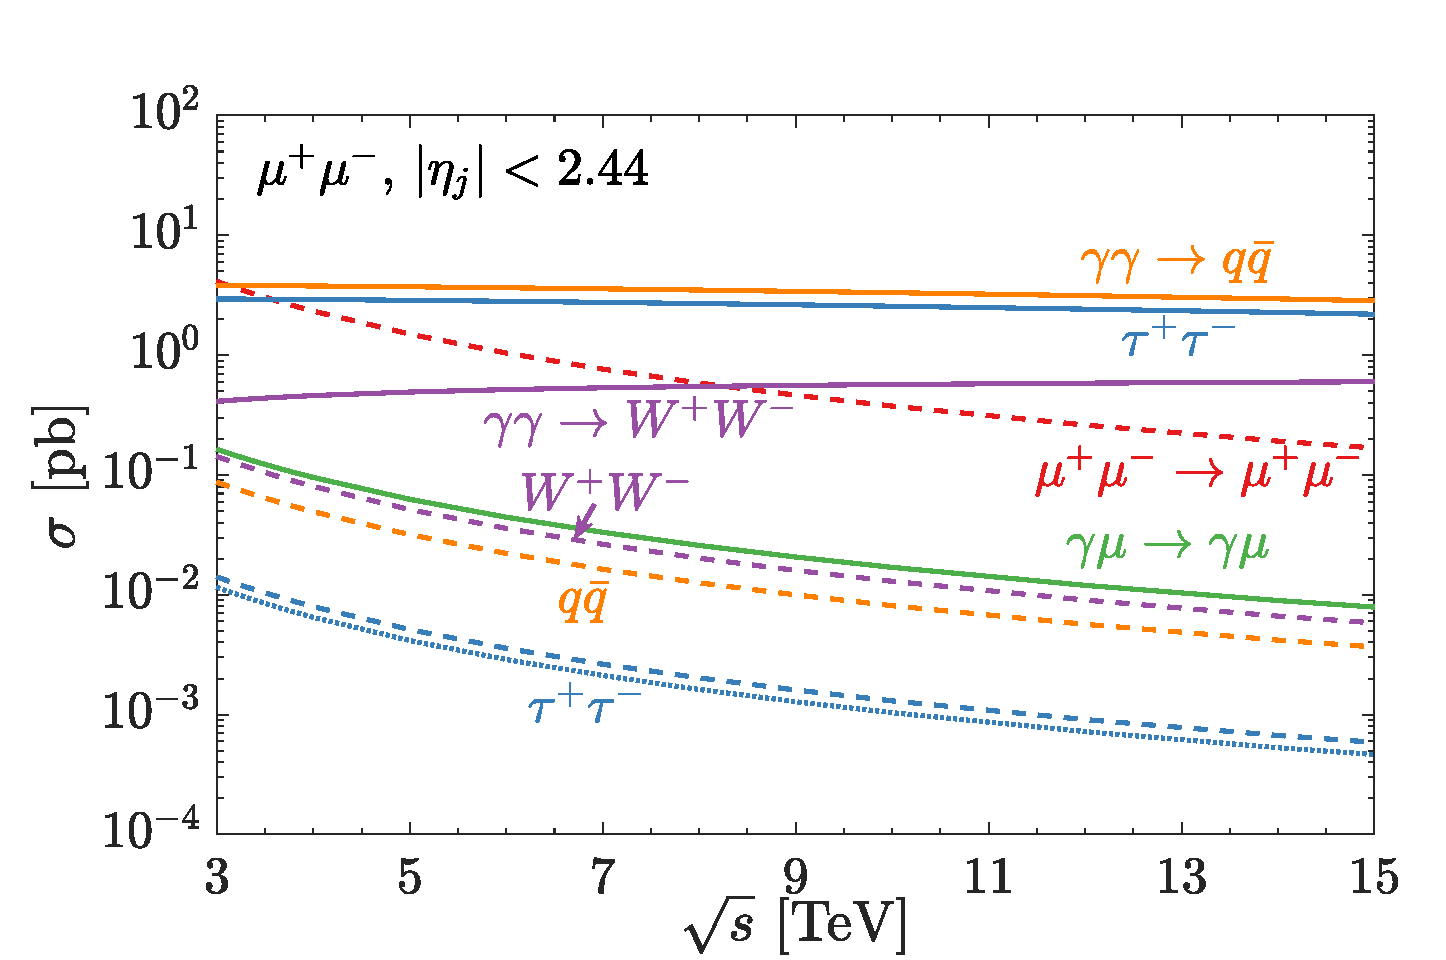
\includegraphics[width=0.8\textwidth]{figs/sigma_mmCollider_c10_3pt_s20}
		\end{column}
	\end{columns}
\end{frame}


% %%%%%%%%%%%%%%%%%%%%%%%%%%%%%%%%%%%%%%%%%%%%
% % Traditional Background
% %%%%%%%%%%%%%%%%%%%%%%%%%%%%%%%%%%%%%%%%%%%%
% \begin{frame}{A high-energy lepton collider at first glance (II)}
% 	\vspace{1mm}\textcolor{PittRoyal}{\bf What are the dominant processes at a high-energy lepton collider? }
% 	\begin{columns}
% 		\begin{column}{0.7\textwidth}
% 		\begin{itemize}
% 			\item Leading-order: $\ell^+\ell^- \to \ell^+\ell^-,\,\tau^+\tau^-,\,q{\bar q},\, W^+W^-$, and $\gamma \ell \to \gamma \ell$
% 			\item $\gamma \gamma$ scatterings: $\gamma\gamma \to \tau^+\tau^-,\,q{\bar q},\, W^+W^-$
% 		\end{itemize}
% 		\hspace{8mm}\textcolor{PittRoyal}{\bf $\bullet$ Need some cuts: }
% 		\begin{itemize}
% 			\item Detector angle: $\theta_{\rm cut}=5^\circ\,(10^\circ)\Longleftrightarrow |\eta|<3.13 (2.44)$ 
% 			\item Threshold: $m_{ij}>20$ GeV
% 			\item Need a $p_T$ cut to separate from the nonperturbative hadronic production
% 			\bib{ Drees and Godbole, PRL 67, 1189; Chen, Barklow, and Peskin, hep-ph/9305247;T. Barklow, etal, LCD-2011-020}
% 			\begin{small}
% 			\begin{eqnarray}
% 				p_T>\left(4+\sqrt s/3 \,{\rm TeV}\right)\,{\rm GeV}\nonumber 
% 			\end{eqnarray}
% 			\end{small}
% 		\end{itemize}
% 		\end{column}
% 		\begin{column}{0.42\textwidth}
% 			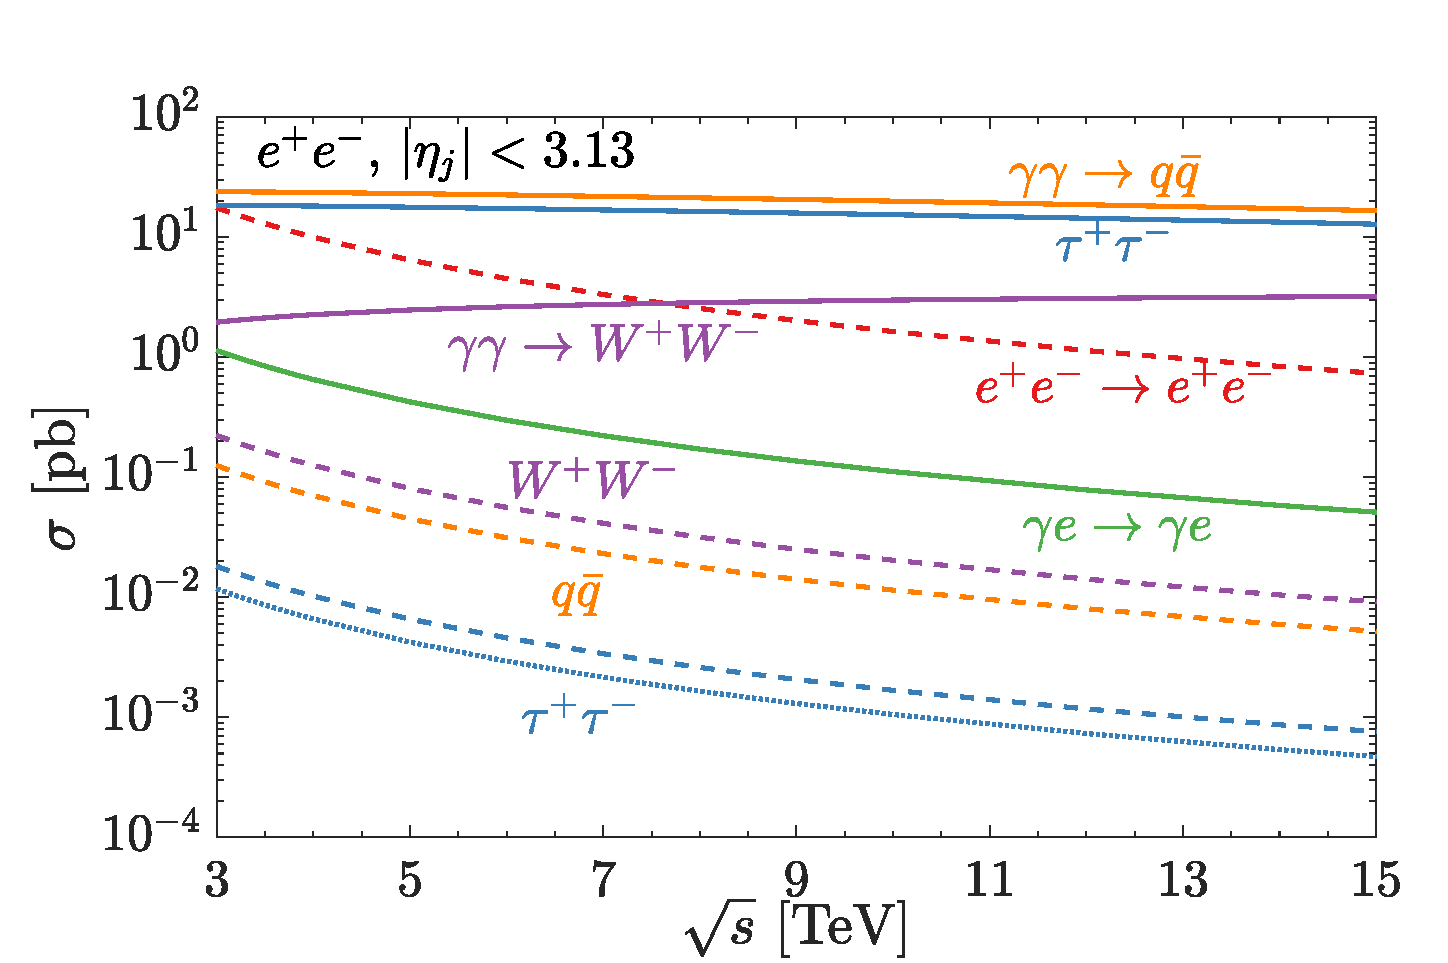
\includegraphics[width=0.8\textwidth]{figs/sigma_eeCollider_c5_3pt_s20}
% 			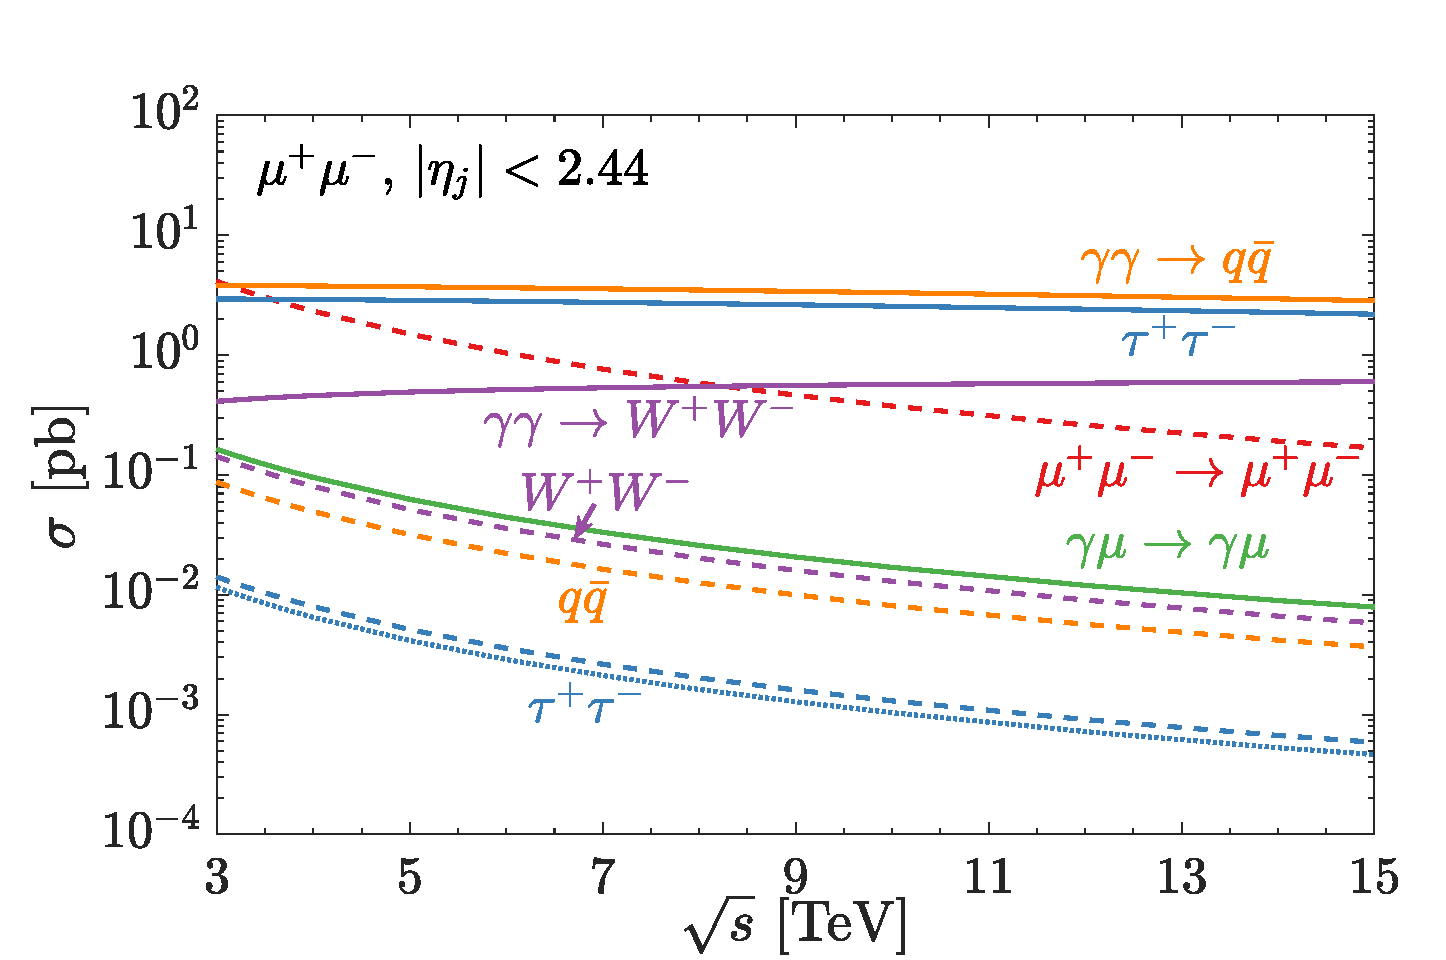
\includegraphics[width=0.8\textwidth]{figs/sigma_mmCollider_c10_3pt_s20}
% 		\end{column}
% 	\end{columns}
% \end{frame}

\subsection{Electroweak PDF and its evolution}
%%%%%%%%%%%%%%%%%%%%%%%%%%%%%%%%%%%%%%%%%%%%
% Go beyond EPA
%%%%%%%%%%%%%%%%%%%%%%%%%%%%%%%%%%%%%%%%%%%%
\begin{frame}
	% \frametitle{Go beyond the EPA at high-energy lepton colliders}
	% \vspace{3mm}\textcolor{PittRoyal}{\bf What are the dominant processes at a high-energy muon collider? }
	\begin{columns}
		\begin{column}[t]{0.48\textwidth}
			\hspace{3mm}\vspace{1mm}\textcolor{black}{\bf People have been doing: }
			\begin{itemize}
				\item $\ell^+\ell^-$ annihilation
				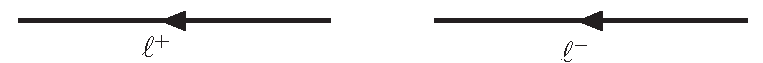
\includegraphics[width=0.8\textwidth]{figs/mm_collision}
				\item EPA and ISR
				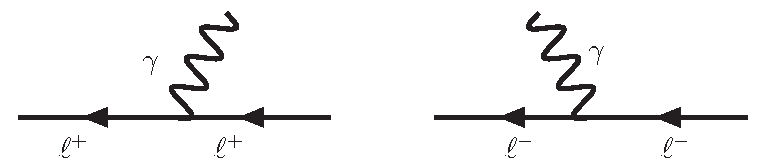
\includegraphics[width=0.8\textwidth]{figs/ISR_collision}
				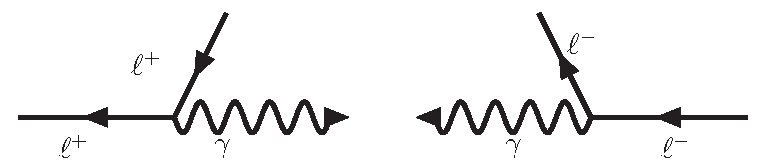
\includegraphics[width=0.8\textwidth]{figs/EPA_collision}
				\item ``Effective W Approx.'' (EWA)\\
				\bib{G. Kane, W. Repko, and W. Rolnick, PLB 148 (1984) 367}\\
				\bib{S. Dawson, NPB 249 (1985) 42}
				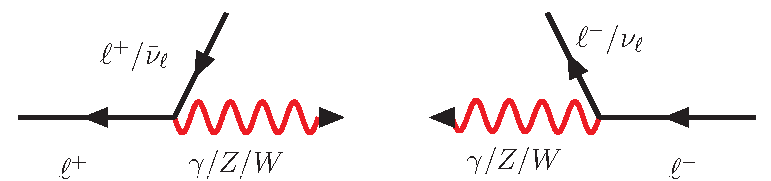
\includegraphics[width=0.8\textwidth]{figs/EWA_collision}
			\end{itemize}
		\end{column}
		\begin{column}[t]{0.5\textwidth}
			\hspace{3mm}\vspace{1mm}\textcolor{PittRoyal}{\bf We will add: }\\
			\hspace{4mm}\bib{T. Han, Y. Ma, K.Xie 2007.14300, 2103.09844}
			\begin{itemize}
				\item Above $\mu_{\rm QCD}$: QED$\otimes$QCD\\
				\textcolor{PittRoyal}{ $q/g$ emerge}\\
				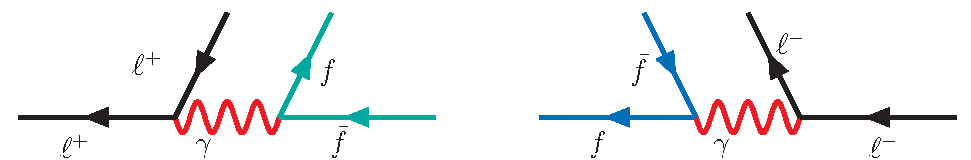
\includegraphics[width=0.8\textwidth]{figs/qq_collision}
				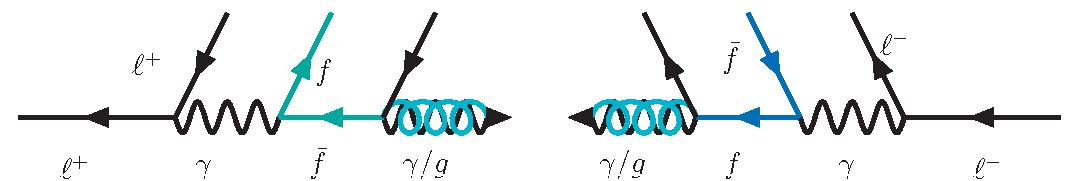
\includegraphics[width=0.8\textwidth]{figs/gg_collision}
				\item Above $\mu_{\rm EW}= M_Z$: EW$\otimes$QCD\\
				\textcolor{PittRoyal}{EW partons emerge}
				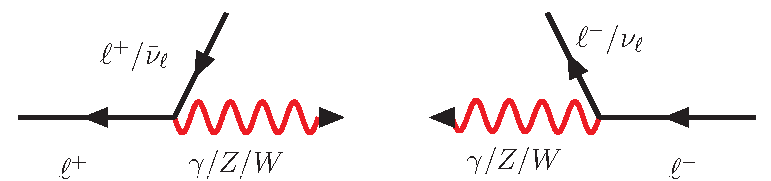
\includegraphics[width=0.8\textwidth]{figs/EWA_collision}
				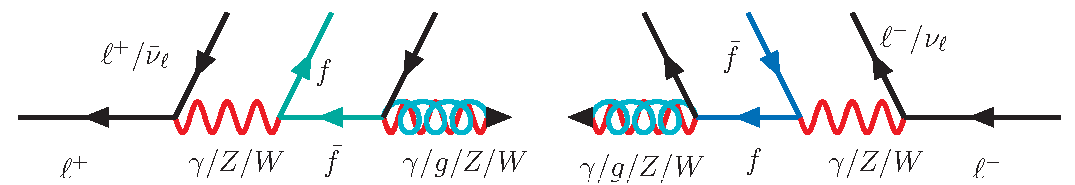
\includegraphics[width=0.8\textwidth]{figs/EW_collision}
			\end{itemize}
		\end{column}
	\end{columns}
	\vspace{1mm}\hspace{5mm}\textcolor{PittRoyal}{\bf In the end, everything is parton, i.e.} \textcolor{red}{\bf need the full SM PDFs. }
\end{frame}

%%%%%%%%%%%%%%%%%%%%%%%%%%%%%%%%%%%%%%%%%%%%
% DGLAP
%%%%%%%%%%%%%%%%%%%%%%%%%%%%%%%%%%%%%%%%%%%%
\begin{frame}{The PDF evolution: DGLAP}
	\begin{itemize}
		\item The DGLAP equations
		\begin{equation}\nonumber
		\frac{\dd f_{i}}{\dd\log Q^2}=\sum_{I}\frac{\alpha_I}{2\pi}\sum_{j}P^{I}_{ij}\otimes f_j
		\end{equation}
		\item The initial conditions
		\beq\nonumber
		f_{\ell/\ell}(x,m_{\ell}^2)=\delta(1-x)
		\eeq	
		\item Three regions and two matchings
		\begin{itemize}
			\item  $m_{\ell}<Q<\muQCD$: QED 
			\item $Q=\muQCD\lesssim1$ GeV: $f_{q}\propto P_{q\gamma}\otimes f_{\gamma}, f_{g}=0$	
			\item $\muQCD<Q<\muEW$: QED$\otimes$QCD
			\item $Q=\muEW=M_Z$: $f_{\nu}=f_{t}=f_{W}=f_{Z}=f_{\gamma Z}=0$	
			\item $\muEW<Q$: EW$\otimes$QCD.
		\end{itemize}
		\begin{equation}\nonumber
		\begin{pmatrix}
		f_B\\ f_{W^3}\\ f_{BW^3}
		\end{pmatrix}=\begin{pmatrix}
		c_W^2 & s_W^2  & -2c_W s_W\\
		s_W^2 & c_W^2  & 2c_W s_W\\
		c_W s_W & -c_W s_W & c_W^2-s_W^2
		\end{pmatrix}
		\begin{pmatrix}
		f_\gamma  \\ f_Z\\ f_{\gamma Z}
		\end{pmatrix}\nonumber
		\end{equation}			
		\item  We work in the $(B,W)$ basis. The technical details can be referred to the backup slides.
		\end{itemize}
\end{frame}

%%%%%%%%%%%%%%%%%%%%%%%%%%%%%%%%%%%%%%%%%%%%
% PDFs
%%%%%%%%%%%%%%%%%%%%%%%%%%%%%%%%%%%%%%%%%%%%
\begin{frame}{The QED$\otimes$QCD PDFs for lepton colliders}
	\begin{columns}
		\begin{column}{0.65\textwidth}
			\begin{itemize}
				\item \textcolor{PittRoyal}{\bf Electron PDFs}: $f_{e_{\rm val}},\, f_\gamma,\, f_{\ell_{\rm sea}},\, f_q,\, f_g$
				\item Scale uncertainty: $10\%$ for $f_{g/e}$
				\item The averaged momentum fractions $\langle x_i\rangle=\int xf_i(x)\dd x$
				\begin{table}[tb]
					\scalebox{0.7}{
					\begin{tabular}{|c|c|c|c|c|c|}
						\hline
						$Q(e^\pm)$ & $e_{\textrm{val}}^{}$ & $\gamma$ & $\lsea$ & $q$ & $g$\\
						\hline
						30 GeV &96.6 & 3.20 & 0.069 & 0.080 & 0.023 \\
						50 GeV &96.5 & 3.34 & 0.077 & 0.087 & 0.026 \\
						$M_Z$  &96.3 & 3.51 & 0.085 & 0.097 & 0.028 \\
						\hline
					\end{tabular}}
				\end{table}
			\end{itemize}
		\end{column}
		\begin{column}{0.45\textwidth}
			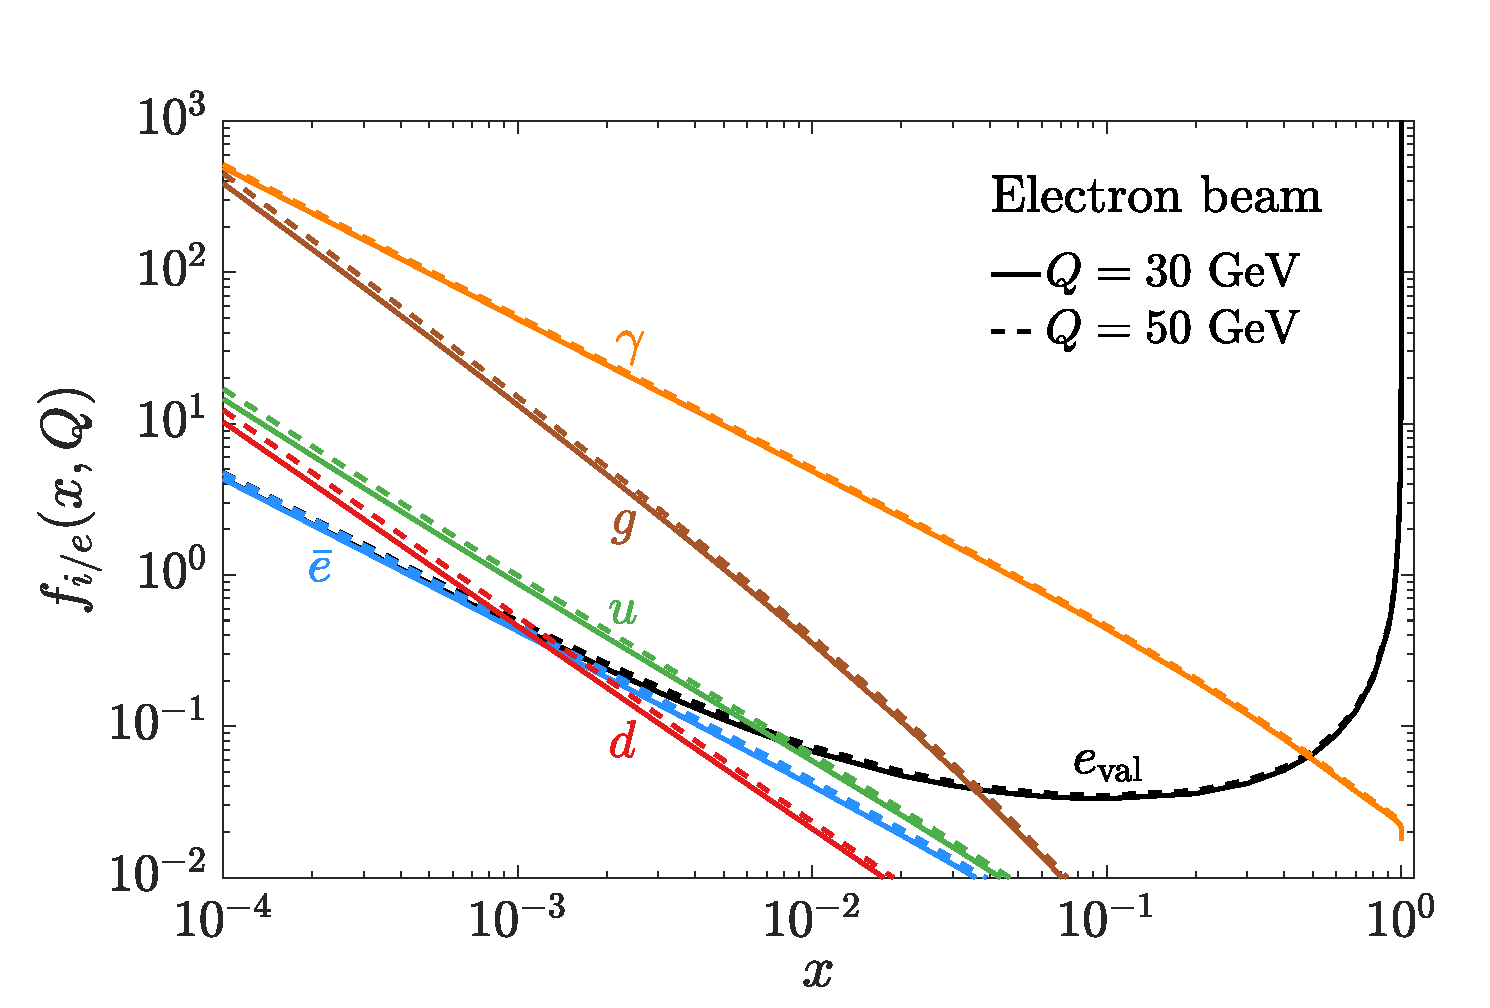
\includegraphics[width=0.85\textwidth]{figs/QECDe}
		\end{column}
	\end{columns}
	\begin{columns}
		\begin{column}{0.65\textwidth}
			\begin{itemize}
				\item \textcolor{PittRoyal}{\bf Muon PDFs}: $f_{\mu_{\rm val}},\, f_\gamma,\, f_{\ell_{\rm sea}},\, f_q,\, f_g$
				\item Scale uncertainty: $20\%$ for $f_{g/\mu}$
				\item The averaged momentum fractions $\langle x_i\rangle=\int xf_i(x)\dd x$
				\begin{table}[tb]
					\scalebox{0.7}{
					\begin{tabular}{|c|c|c|c|c|c|}
						\hline
						$Q(\mu^\pm)$ & $\mu_{\textrm{val}}^{}$ & $\gamma$ & $\lsea$ & $q$ & $g$\\
						\hline
						30 GeV & 98.2 & 1.72 & 0.019 & 0.024 & 0.0043 \\
						50 GeV & 98.0 & 1.87 & 0.023 & 0.029 & 0.0051\\
						$M_Z$  & 97.9 & 2.06 & 0.028 & 0.035 & 0.0062 \\
						\hline
					\end{tabular}}
				\end{table}
			\end{itemize}
		\end{column}
		\begin{column}{0.45\textwidth}
			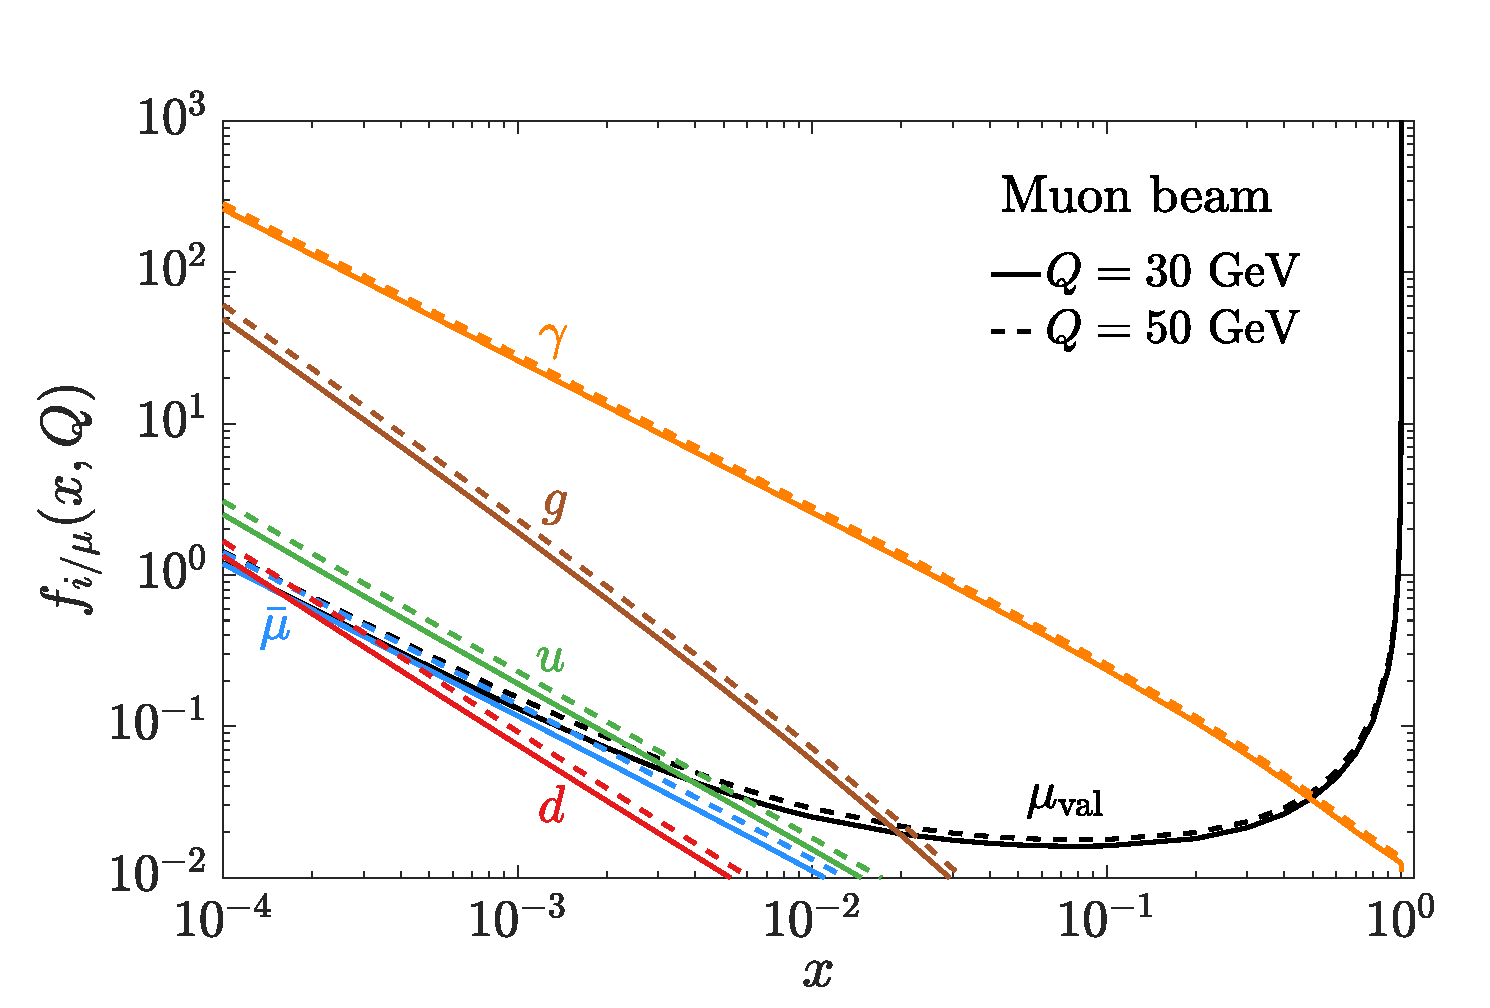
\includegraphics[width=0.85\textwidth]{figs/QECDm}
		\end{column}
	\end{columns}
\end{frame}

%%%%%%%%%%%%%%%%%%%%%%%%%%%%%%%%%%%%%%%%%%%%
% EWPDF
%%%%%%%%%%%%%%%%%%%%%%%%%%%%%%%%%%%%%%%%%%%%
\begin{frame}
	\frametitle{The PDFs of a lepton beyond the EW scale}
	\begin{columns}
		\begin{column}{0.6\textwidth}
			\begin{itemize}
				\item \textcolor{PittRoyal}{\bf All SM particles are partons}\\
				\bib{T. Han, Y. Ma, K.Xie 2007.14300, 2103.09844}
				\begin{itemize}
					\item The sea leptonic and quark PDFs show up\\~
					$\nu=\sum_{i}(\nu_i+\bar{\nu}_i)$,\\~
					$\lsea=\bar{\mu}+\sum_{i\neq\mu}(\ell_i+\bar{\ell}_i)$,\\~ 
					$q=\sum_{i=d}^t(q_i+\bar{q}_i)$\\
					\textcolor{PittRoyal}{There is even neutrino due to the EW sector}	
					\end{itemize}
				\item $W_L$ does not evolve at the leading order. 
				\item The EW correction is not small:
				$\sim 50\%$ ($100\%$) for $f_{d/e}$ ($f_{d/\mu}$) due to the relatively {\bf large SU(2) gauge coupling}. \bib{T. Han, Y. Ma, K.Xie 2103.09844}
				\item Scale uncertainty: $\sim 15\%$ ($20\%$) between $Q=3$ TeV and $Q=5$ TeV \\
			\end{itemize}
		\end{column}
		\begin{column}{0.45\textwidth}
		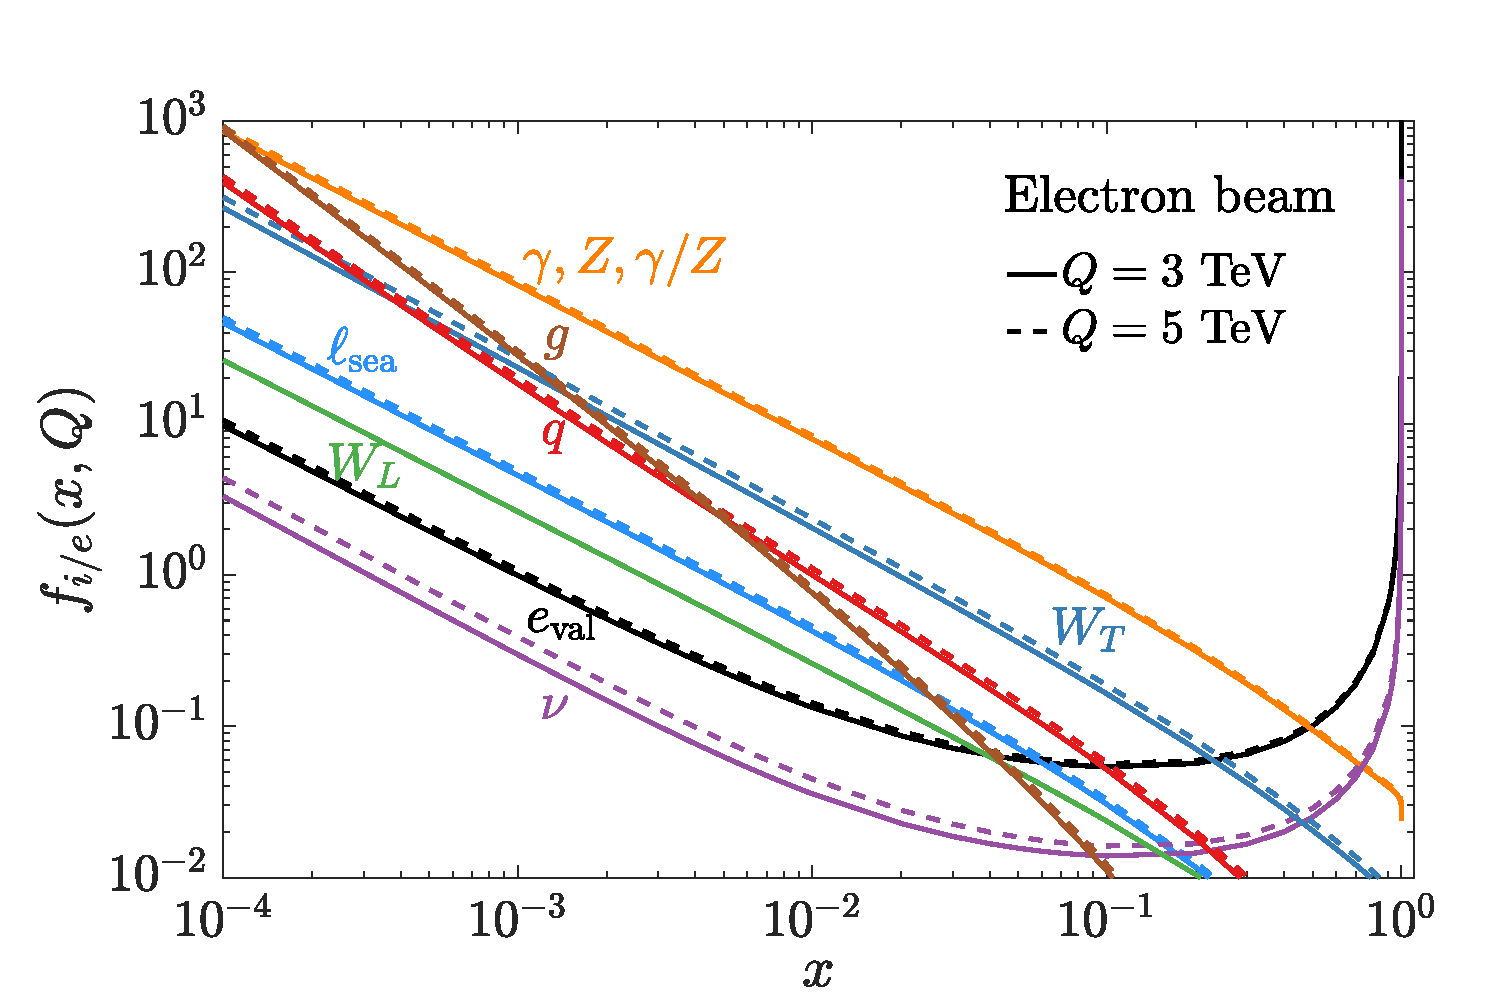
\includegraphics[width=0.85\textwidth]{figs/EWPDFe.pdf}
		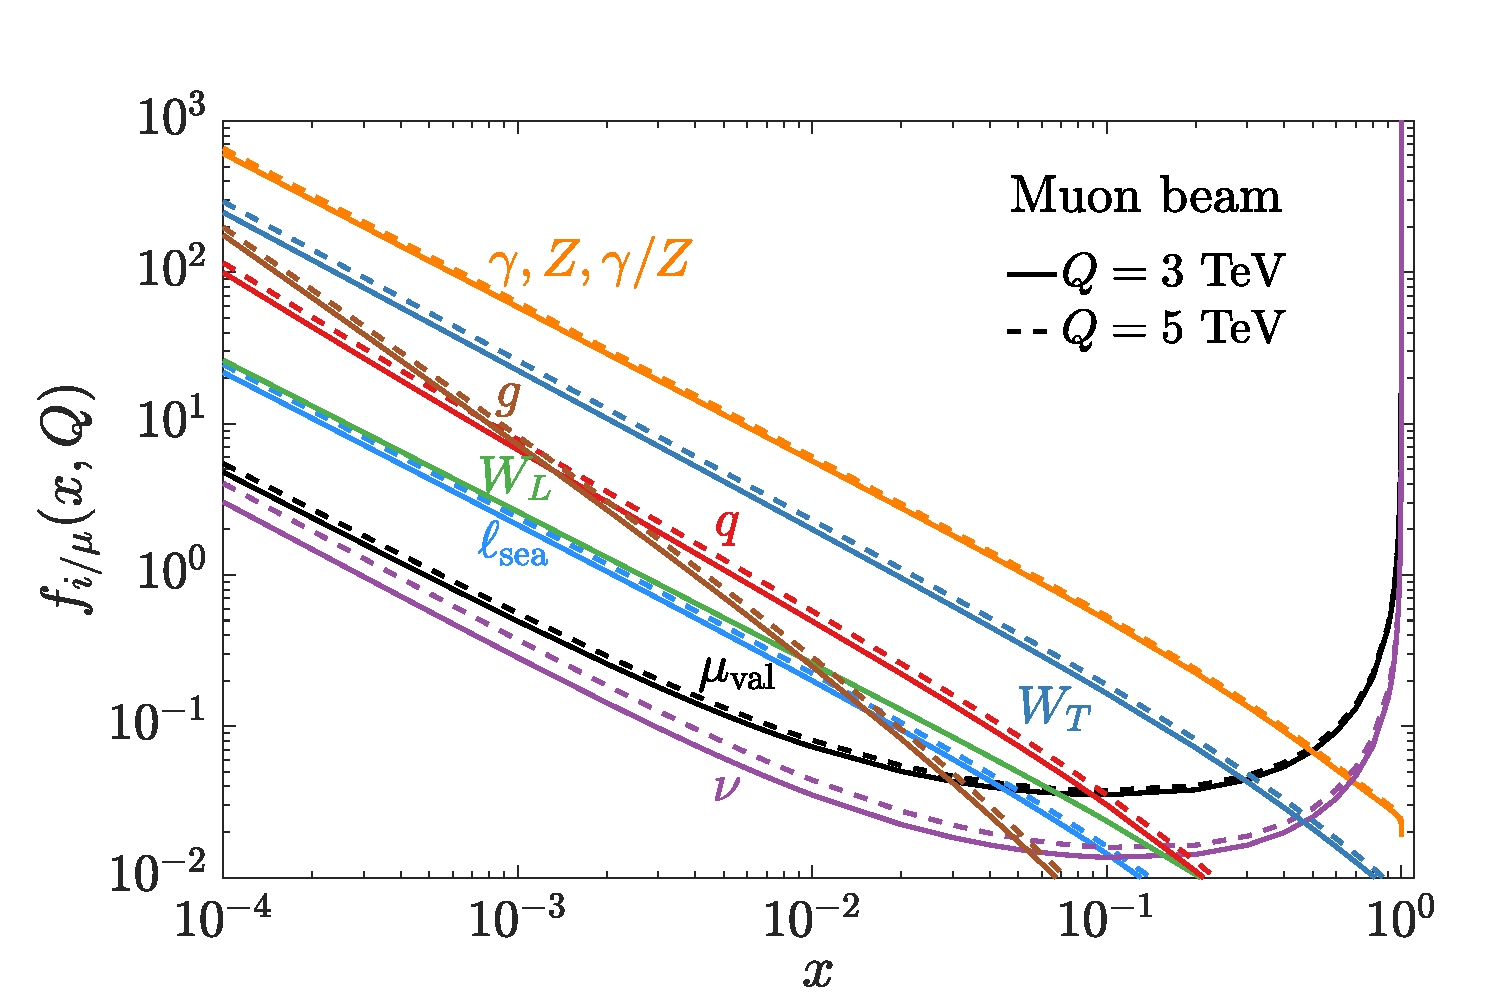
\includegraphics[width=0.85\textwidth]{figs/EWPDFm.pdf}
		\end{column}
	\end{columns}
\end{frame}

\subsection{The SM expectation of future high-energy lepton colliders}
%%%%%%%%%%%%%%%%%%%%%%%%%%%%%%%%%%%%%%%%%%%%
% Lumi
%%%%%%%%%%%%%%%%%%%%%%%%%%%%%%%%%%%%%%%%%%%%
\begin{frame}{Parton luminosities at high-energy lepton colliders}
	\begin{columns}
		\begin{column}{0.66\textwidth}
			\hspace{3mm}\textcolor{PittRoyal}{\bf A $3$ TeV $e^+e^-$ machine and a $10$ TeV $\mu^+\mu^-$ machine}
			\begin{itemize}
				\item Partonic luminosities for
				\begin{eqnarray}
					\ell^+\ell^-,\, \gamma\ell, \, \gamma\gamma,\, qq,\, \gamma q,\, \gamma g,\, gq,\ {\rm and}\ gg \nonumber
				\end{eqnarray}
				\item $\gamma \gamma$ gives the largest partonic luminosity
				\item The luminosity of $\gamma g + \gamma q$ is $\sim 50\%$ ($20\%$) of $\gamma \gamma$
				\item The luminosities of $qq$, $gq$, and $gg$ are $\sim 2\%$ ($0.5\%$) of $\gamma \gamma$
				\item Given the stronger QCD coupling, {\bf sizable QCD cross sections are expected}.
				\item Scale uncertainty is $\sim 20\%$ ($50\%$) for photon (gluon) initiated processes.
			\end{itemize}
		\end{column}
		\begin{column}{0.44\textwidth}
			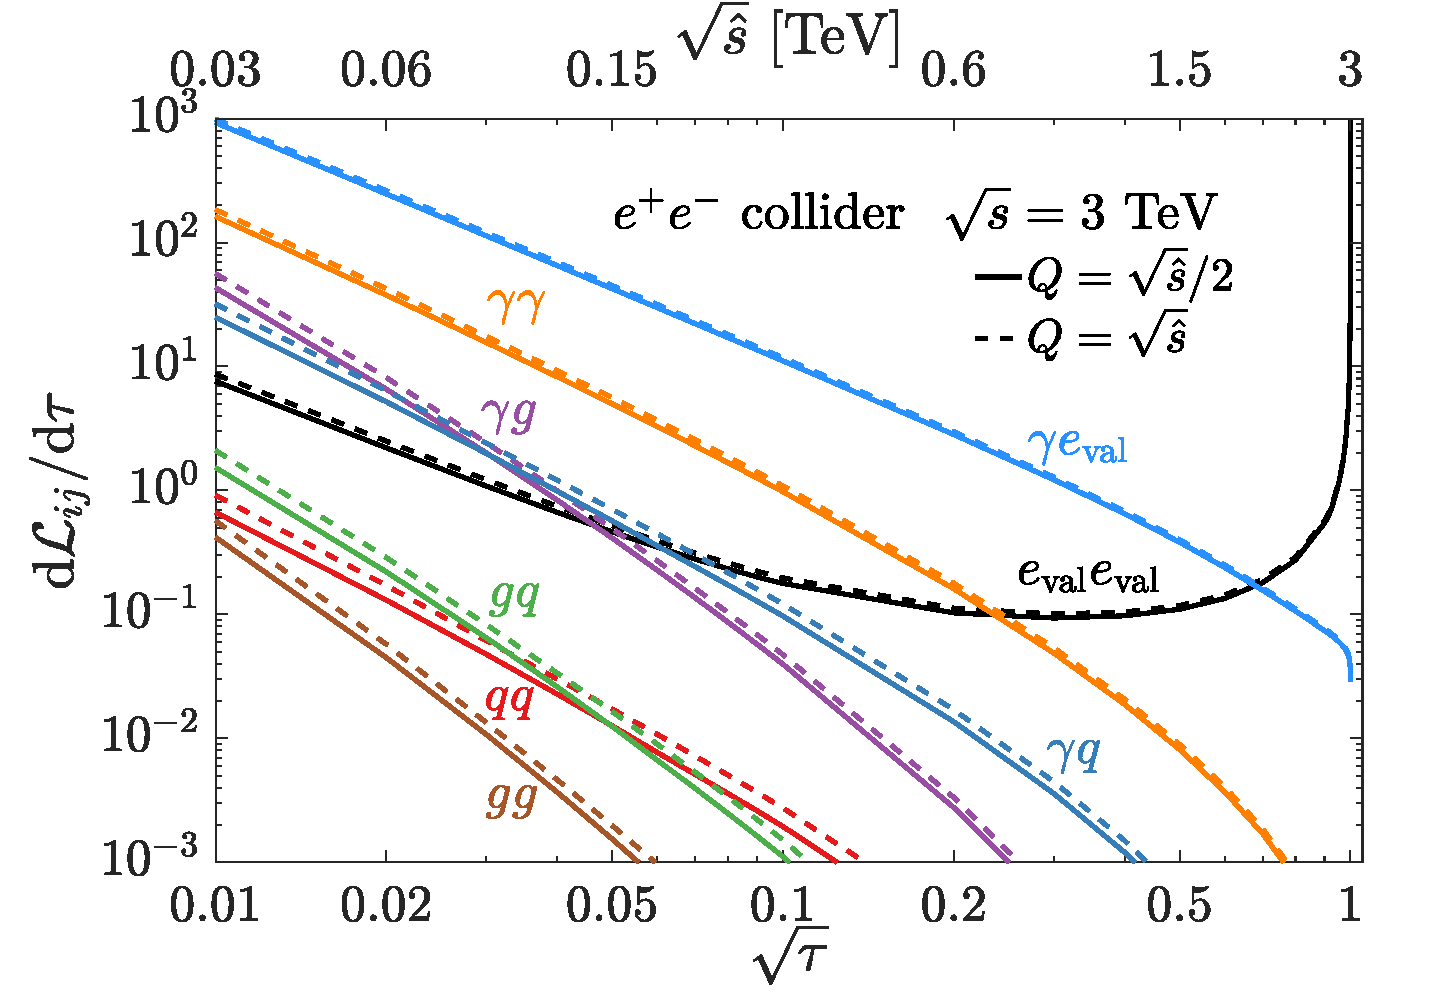
\includegraphics[width=0.84\textwidth]{figs/lumi_e_3TeV}
			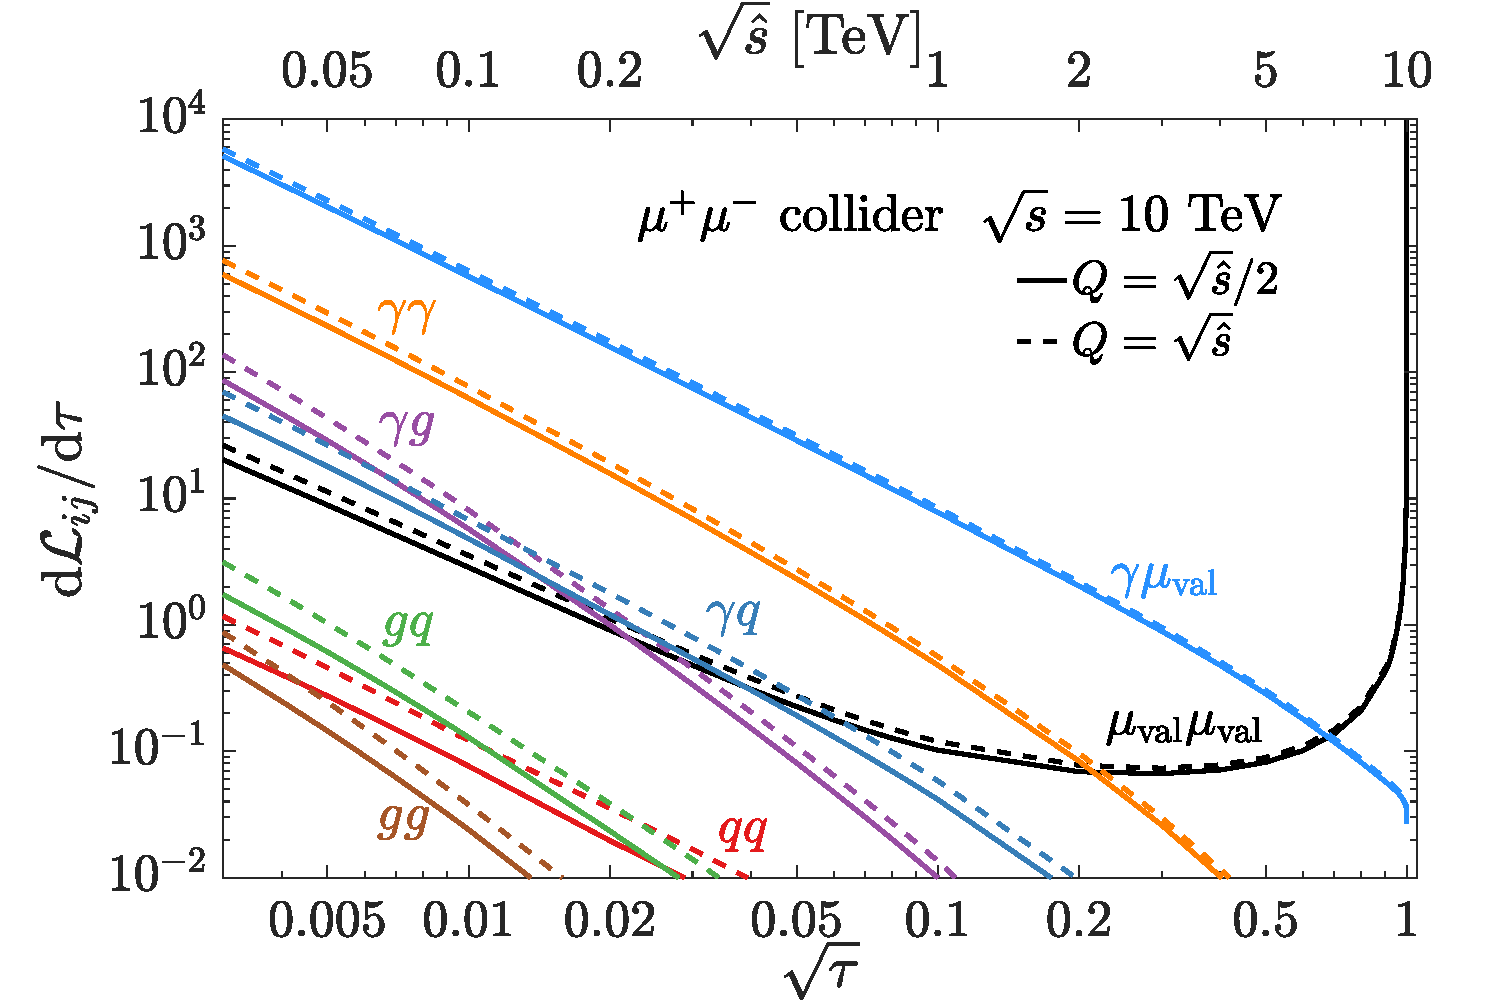
\includegraphics[width=0.84\textwidth]{figs/lumi_mu_10TeV}
		\end{column}
	\end{columns}
\end{frame}

%%%%%%%%%%%%%%%%%%%%%%%%%%%%%%%%%%%%%%%%%%%%
% di-jet cross section
%%%%%%%%%%%%%%%%%%%%%%%%%%%%%%%%%%%%%%%%%%%%
\begin{frame}{Jet production at possible lepton colliders}
	\begin{columns}
		\begin{column}{0.65\textwidth}
			\begin{itemize}
				\item High-$p_T$ range [$p_T>\left(4+\sqrt s/3 \,{\rm TeV}\right)\,{\rm GeV}$]\\ {\bf perturbatively computable}
				\vspace{-3mm}
				\bea
				&\gamma\gamma \to q\bar q,\ \gamma g \to q\bar{q},~\gamma q\to  gq,\\
				&q q\to qq\ (gg),\ gq\to gq\ {\rm and}\ gg\to gg\ (q\bar{q}).\nonumber
				\eea
				\item Large $\alpha_s\ln(Q^2)$ brings a $6\%\sim 15\%$ ($30\%\sim 40\%$) enhancement if $Q=2 Q$
				\item The QCD contributions result in total cross section. 
				\item $gg$ initiated cross sections are large for the {\bf multiplicity}
				\item $gq$ initiated cross sections are large for the {\bf luminosity}.
				\item $\gamma \gamma$ gives smaller cross sections than the EPA does.
			\end{itemize}
		\end{column}
	\begin{column}{0.44\textwidth}
		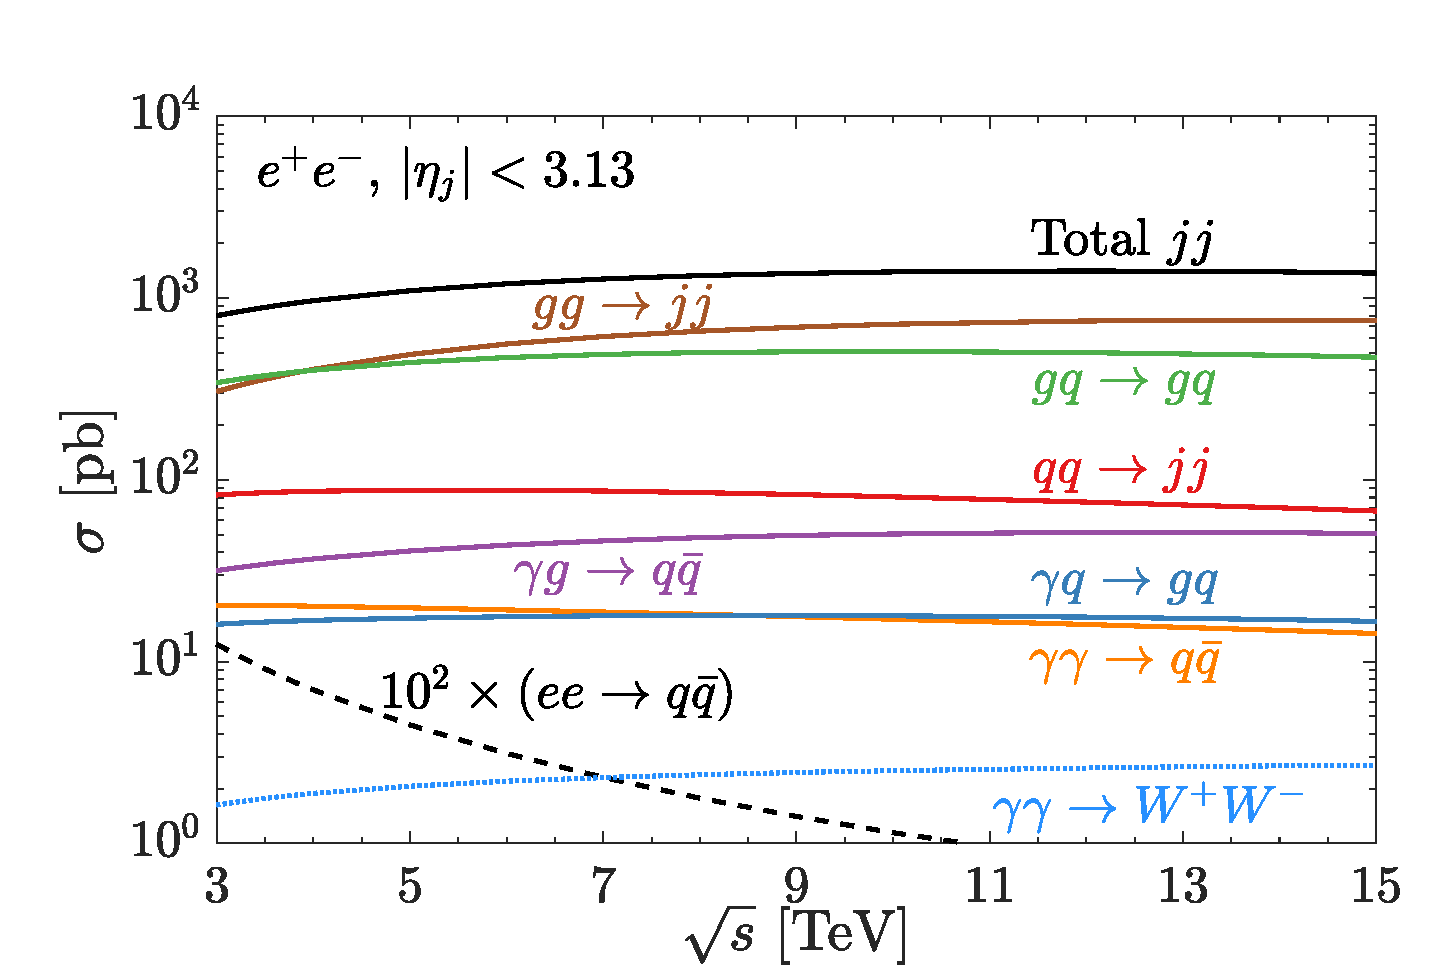
\includegraphics[width=0.85\textwidth]{figs/dijjet_e_5d_3pt_s20}
		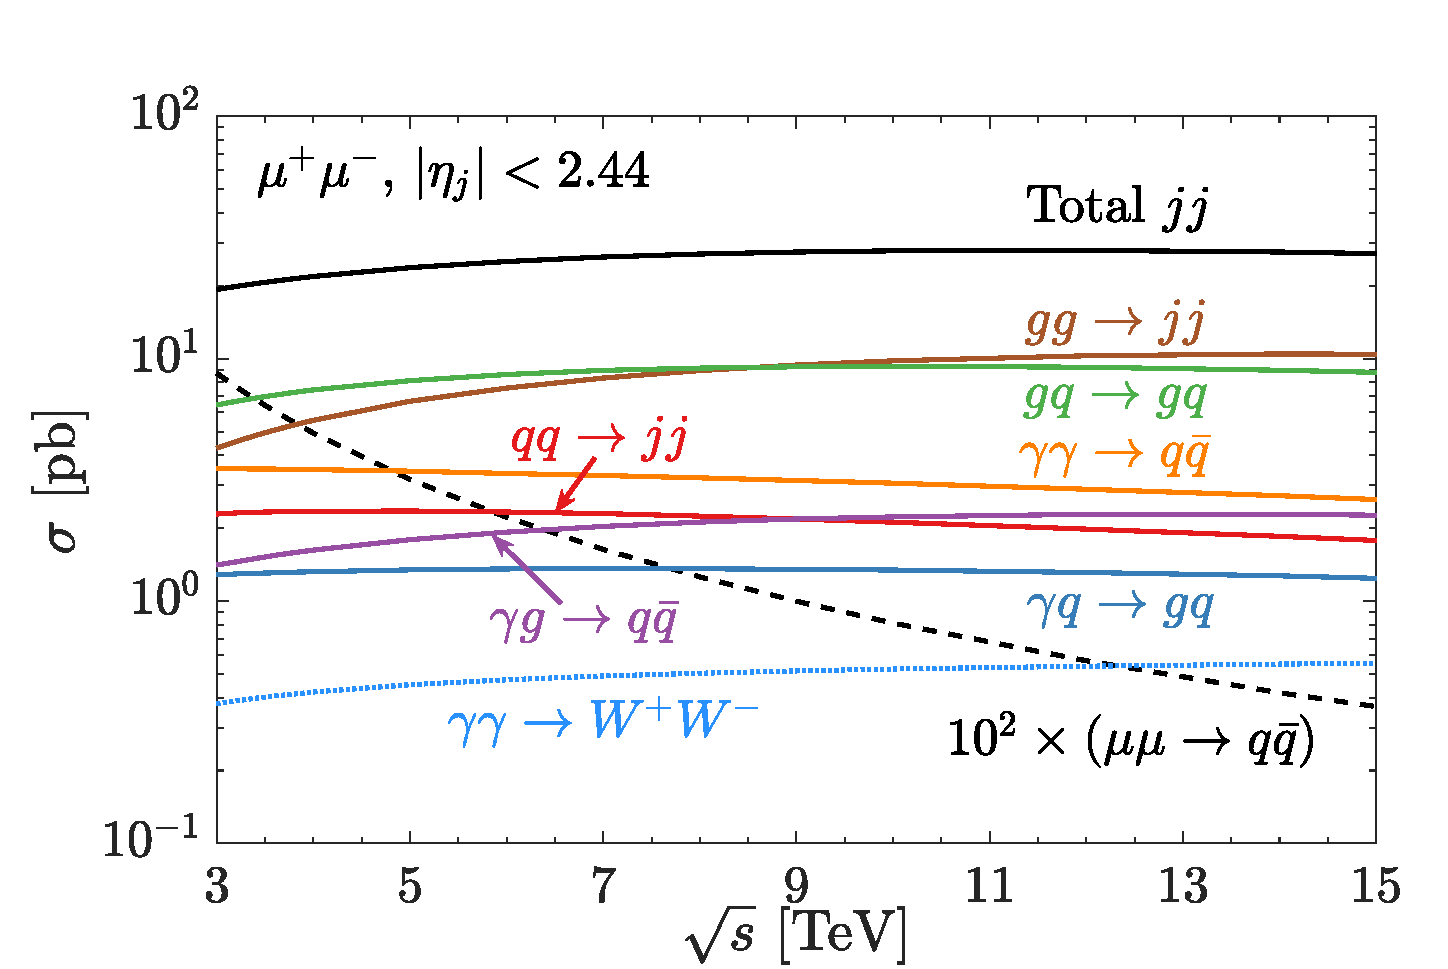
\includegraphics[width=0.85\textwidth]{figs/dijjet_mu_10d_3pt_s20}
		\end{column}
	\end{columns}
\end{frame}

%%%%%%%%%%%%%%%%%%%%%%%%%%%%%%%%%%%%%%%%%%%%
% di-jet distributions
%%%%%%%%%%%%%%%%%%%%%%%%%%%%%%%%%%%%%%%%%%%%
\begin{frame}{Di-jet distributions at a muon collider}
	\vspace{1mm}\textcolor{PittRoyal}{\bf Rather a conservative set up: $\theta =10^\circ$}
	\begin{itemize}
		\item Some physics:\\
		Two different mechanisms: \textcolor{PittRoyal}{\bf $\mu^+\mu^-$ annihilation} VS \textcolor{PittGold}{\bf Fusion processes}
		\begin{itemize}
			\item Annihilation is more than 2 orders of magnitude smaller than fusion process.
			\item Annihilation peaks at $m_{ij}\sim {\sqrt s}$; 
			\item Fusion processes peak near $m_{ij}$ threshold.
			\item Annihilation is very central, spread out due to ISR;
			\item Fusion processes spread out, especially for $\gamma q$ and $\gamma g$ initiated ones.
		\end{itemize}
	\end{itemize}
	\begin{columns}
		\begin{column}{0.44\textwidth}
			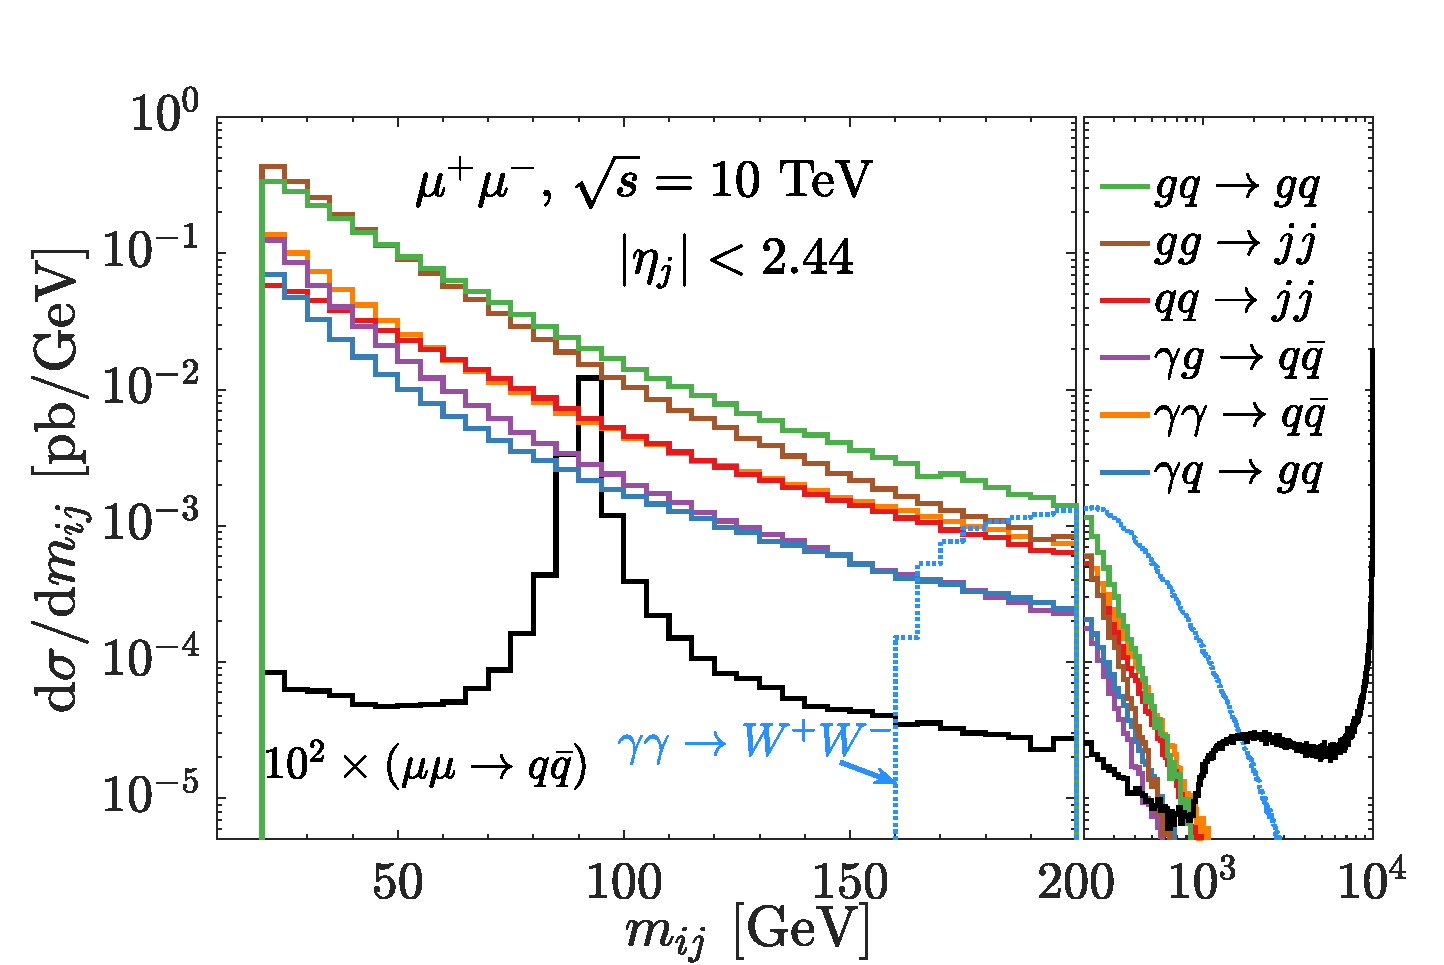
\includegraphics[width=0.88\textwidth]{figs/dMjj_mu10TeV_10d_3pt_s20}
	\end{column}
	\hspace{-5mm}
	\begin{column}{0.44\textwidth}
		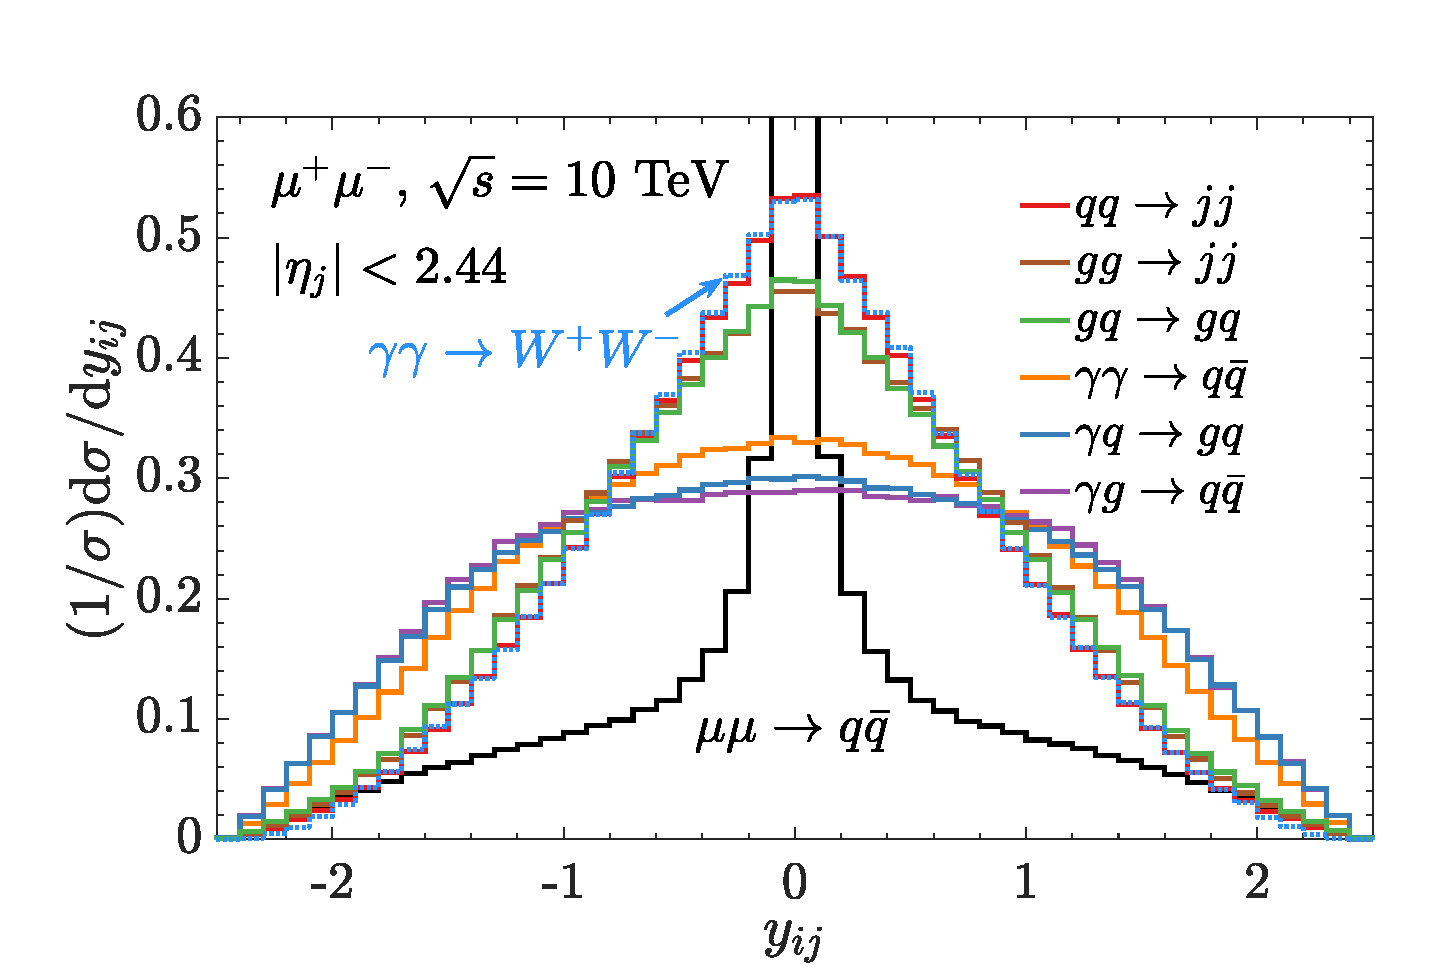
\includegraphics[width=0.88\textwidth]{figs/dYjj_mu10TeV_10d_3pt_s20_Norm}
		\end{column}
	\end{columns}
\end{frame}

%%%%%%%%%%%%%%%%%%%%%%%%%%%%%%%%%%%%%%%%%%%%
% Inclusive jet distributions
%%%%%%%%%%%%%%%%%%%%%%%%%%%%%%%%%%%%%%%%%%%%

\begin{frame}{Inclusive jet distributions at a muon collider}
	% \vspace{3mm}\hspace{10mm}\textcolor{PittRoyal}{\bf $\theta =10^\circ$}
\begin{columns}	
	\begin{column}{0.48\textwidth}
		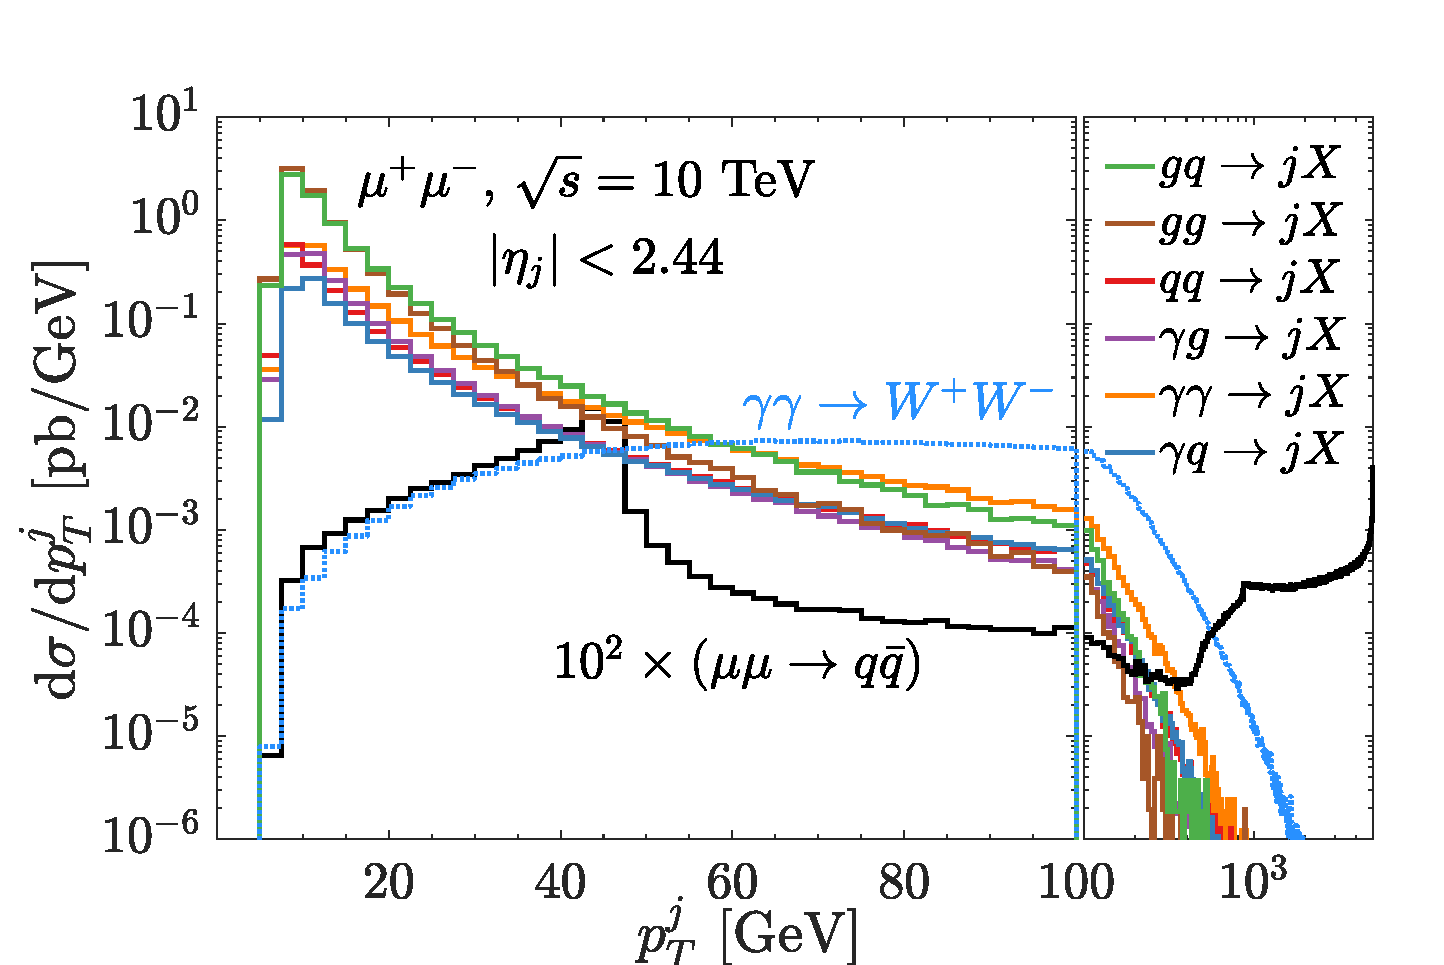
\includegraphics[width=0.88\textwidth]{figs/dPTj_mu10TeV_10d_3pt_s20}
		% 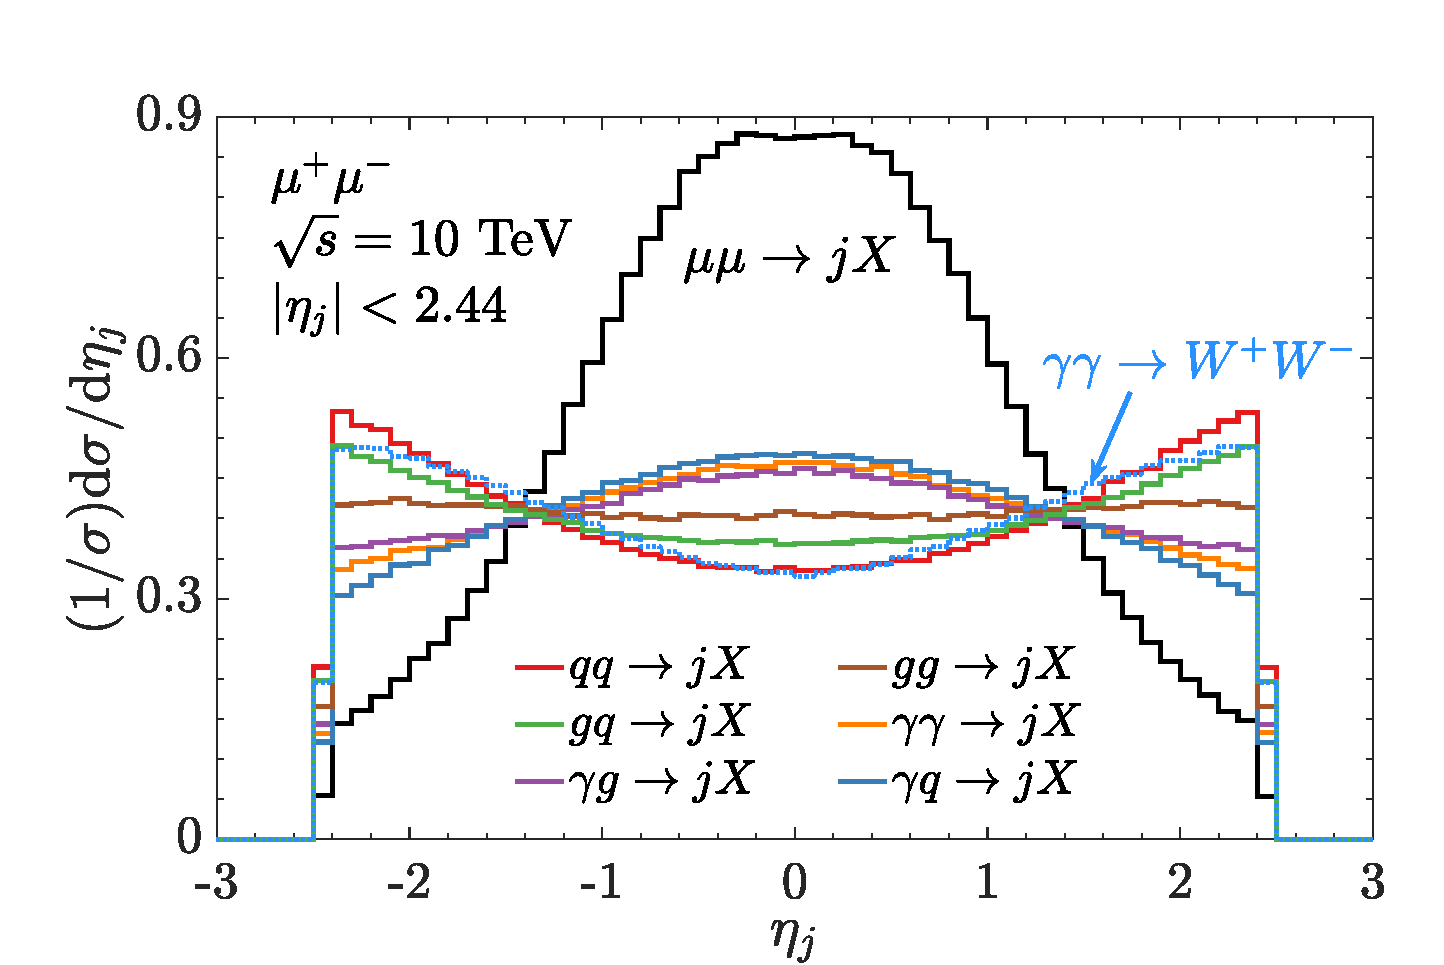
\includegraphics[width=0.88\textwidth]{figs/detaj_mu10TeV_10d_3pt_s20_Norm}
	\end{column}
	\begin{column}{0.48\textwidth}
		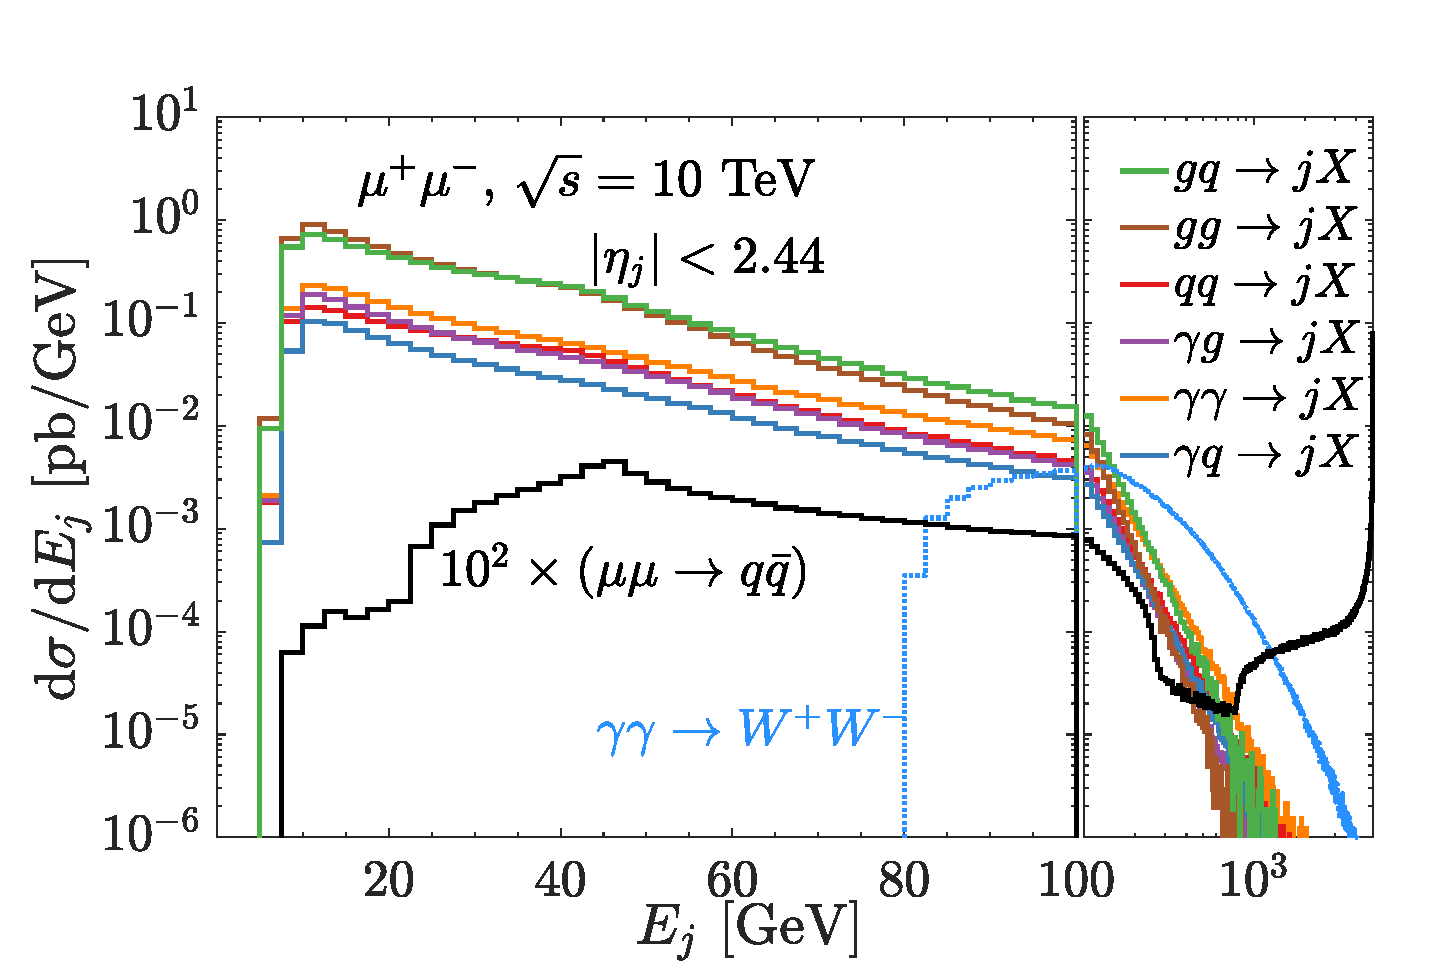
\includegraphics[width=0.88\textwidth]{figs/dEj_mu10TeV_10d_3pt_s20}
	\end{column}
\end{columns}
\textcolor{PittRoyal}{\bf We expect}
\begin{itemize}
	\item Jet production dominates over $WW$ production until $p_T>60$ GeV;
	\item $WW$ production takes over around energy $\sim 200$ GeV.
	% \item QCD contributions are mostly forward-backward; $\gamma \gamma$,  $\gamma q$, and  $\gamma g$ initiated processes are more isotropic.
\end{itemize}
\end{frame}

%%%%%%%%%%%%%%%%%%%%%%%%%%%%%%%%%%%%%%%%%%%%
% Semi-inclusive processes
%%%%%%%%%%%%%%%%%%%%%%%%%%%%%%%%%%%%%%%%%%%%
\begin{frame}
    \frametitle{The full picture: Semi-inclusive processes}
	\begin{columns}	
		\begin{column}{0.48\textwidth}
			\vspace{2mm}\hspace{3mm}\textcolor{PittRoyal}{\bf Just like in hadronic collisions:}\\
			$\mu^+\mu^-\to$ exclusive particles $+$ remnants
			\centering
			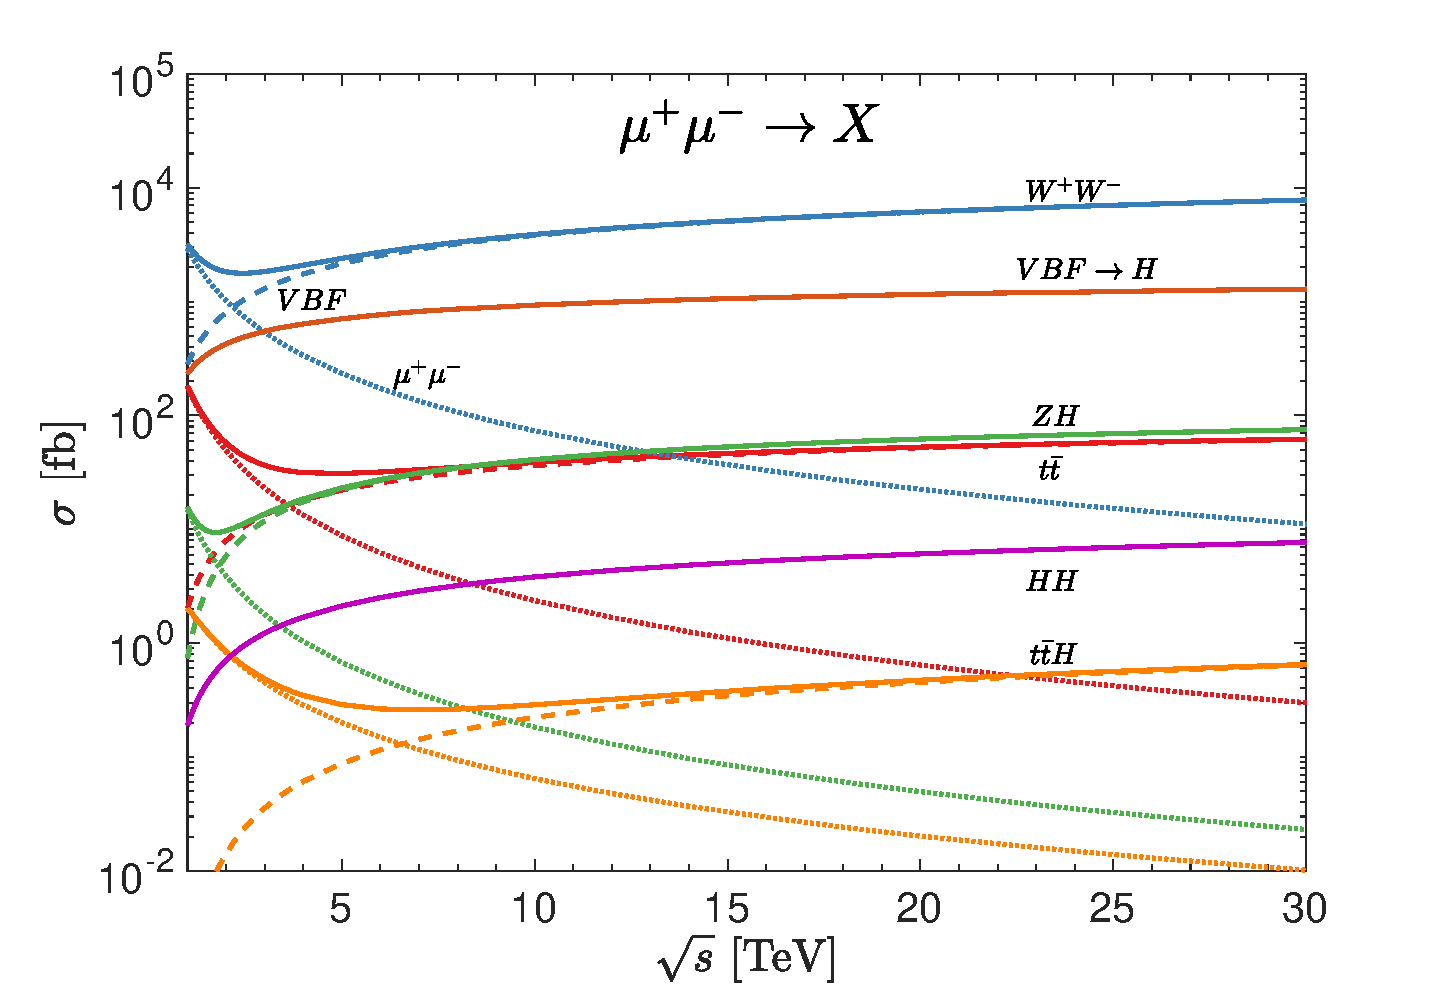
\includegraphics[width=1\textwidth]{figs/sigma_PDF2.pdf}\\
			\hspace{20mm}\bib{T. Han, Y. Ma, K.Xie 2007.14300}
		\end{column}
		\begin{column}{0.42\textwidth}
			\vspace{2mm}\hspace{3mm}\textcolor{PittRoyal}{\bf One example:}
			$\mu^+\mu^-\to t{\bar t}+X$
			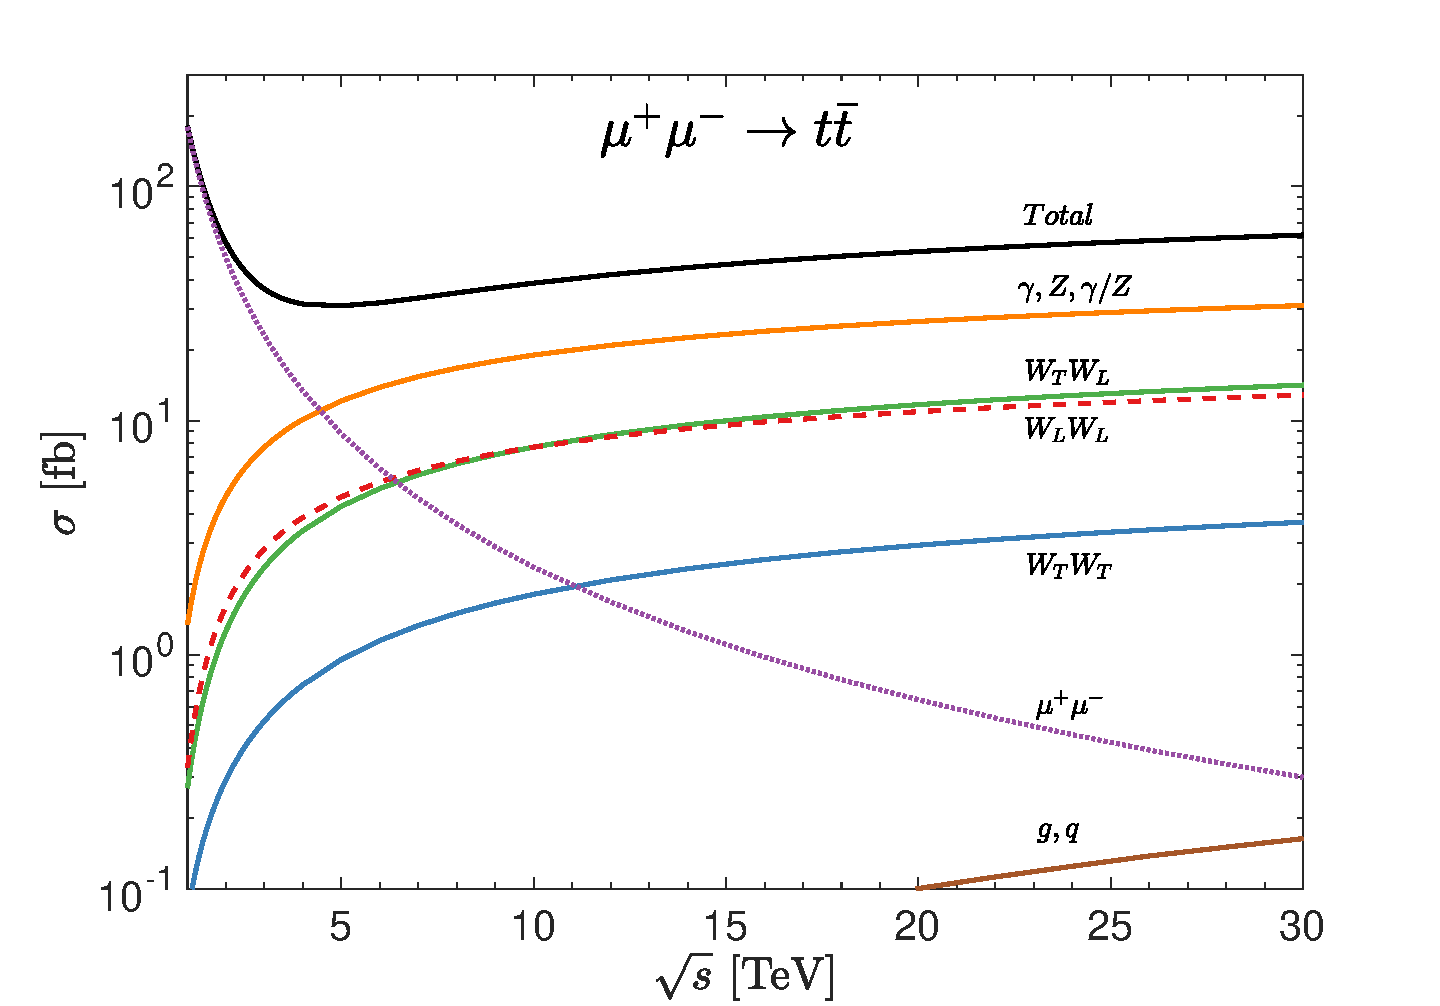
\includegraphics[width=0.8\textwidth]{figs/sigma_tt.pdf}
			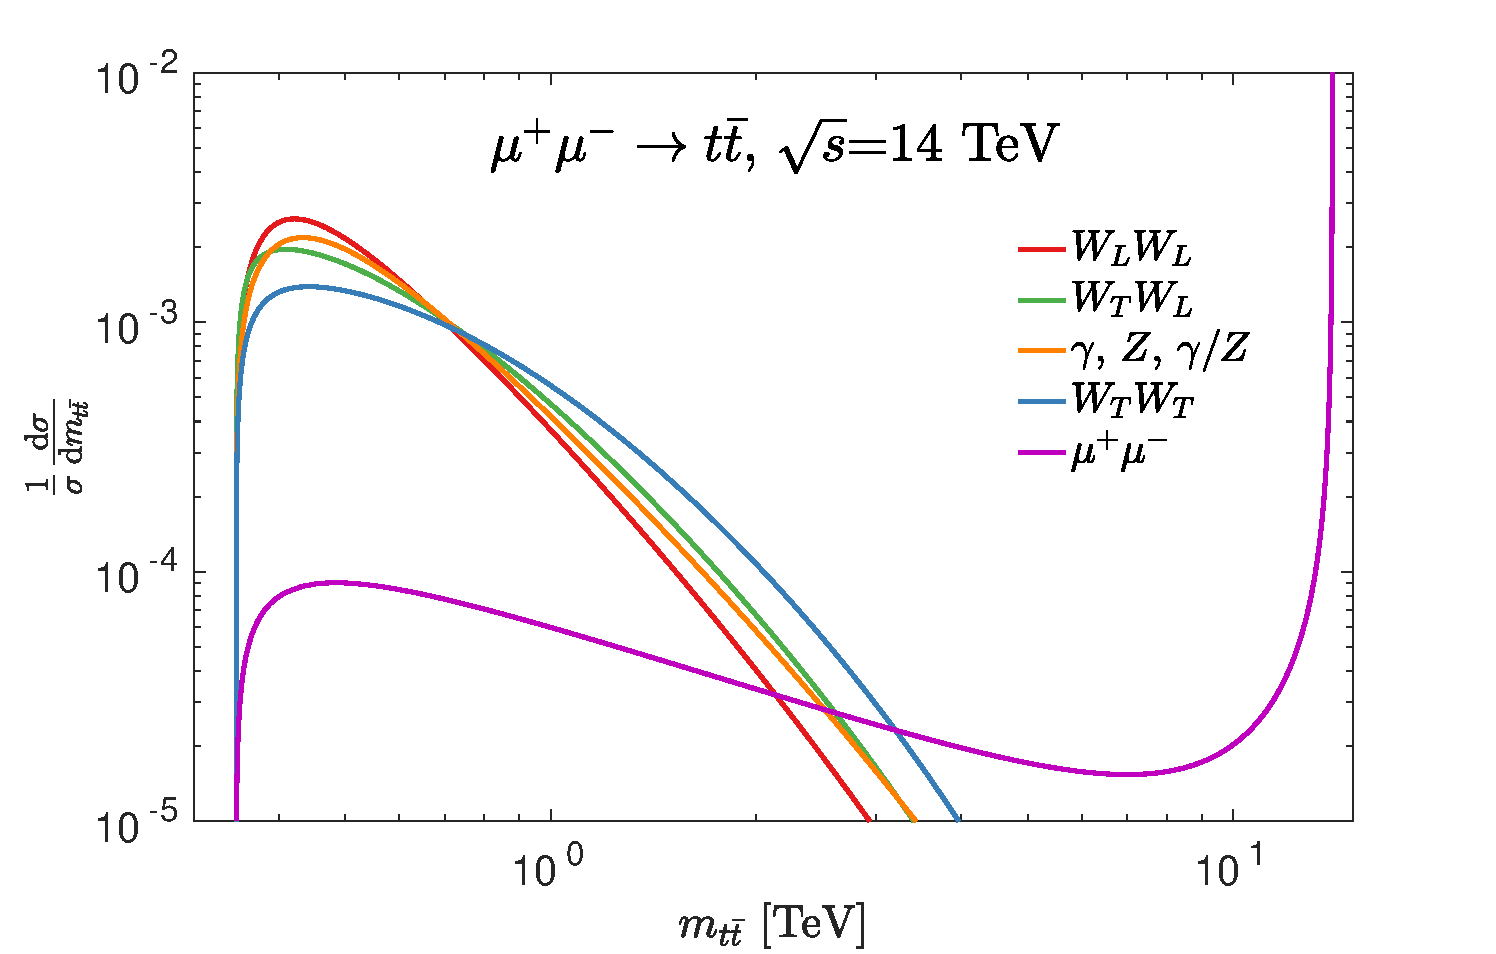
\includegraphics[width=0.8\textwidth]{figs/tt_dmtt.pdf}
		\end{column}
	\end{columns}   
\end{frame}

%% ===========================================
%% ===========================================
\section[Multi-boson productions and Muon Yukawa]{Multi-boson productions at a high-energy muon collider and the Muon-Higgs coupling} 
%% ===========================================
%% ===========================================
\subsection{Multi-boson physics at future high-energy lepton colliders}
%%%%%%%%%%%%%%%%%%%%%%%%%%%%%%%%%%%%%%%%%%%%
%Multi-boson physics
%%%%%%%%%%%%%%%%%%%%%%%%%%%%%%%%%%%%%%%%%%%%
\begin{frame}
	\frametitle{Multi-boson physics}
	\textcolor{PittRoyal}{\bf New phenomenology at a multi-TeV lepton collider}:
	\begin{enumerate}
		\item Multi-boson production (annihilation)
		\item \dots and vector boson fusion ({\bf VBF}) to multi-bosons, \\leading to multi-fermion final states with resonance structure.\\
		\hspace{5mm}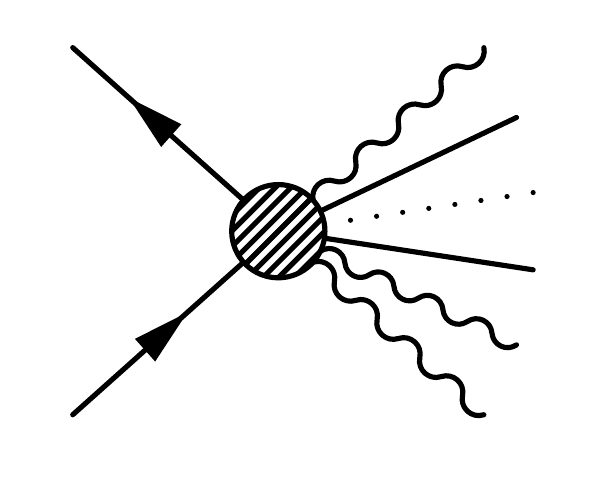
\includegraphics[width=0.23\textwidth]{figs/multiB1.png}
		\hspace{5mm}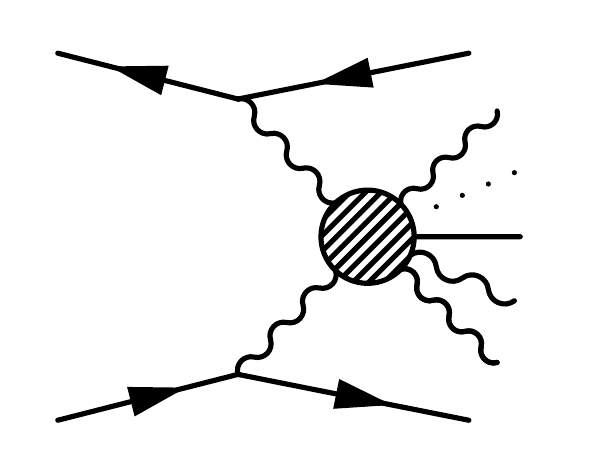
\includegraphics[width=0.23\textwidth]{figs/multiB2.png}
	\end{enumerate}
	\hfill\bib{Barger, Cheung, Han, Phillips 1995}
	\bib{Boos, He, Kilian, Pukhov, Yuan, Zerwas 1998}

	\hspace{5mm}\textcolor{PittRoyal}{\bf Task}:\\
	\hspace{5mm}Measure \textcolor{PittRoyal}{all} interactions of multiple SM particles \textcolor{PittRoyal}{exclusively} and with\\ \hspace{5mm}\textcolor{PittRoyal}{precision}, from threshold to up to $2$ orders of magnitude above EW scale.
\end{frame}

%%%%%%%%%%%%%%%%%%%%%%%%%%%%%%%%%%%%%%%%%%%%
%Annihilation vs VBF
%%%%%%%%%%%%%%%%%%%%%%%%%%%%%%%%%%%%%%%%%%%%
\begin{frame}
	\frametitle{Annihilation vs VBF: Properties (SM)}
	% \vspace{-1mm}
	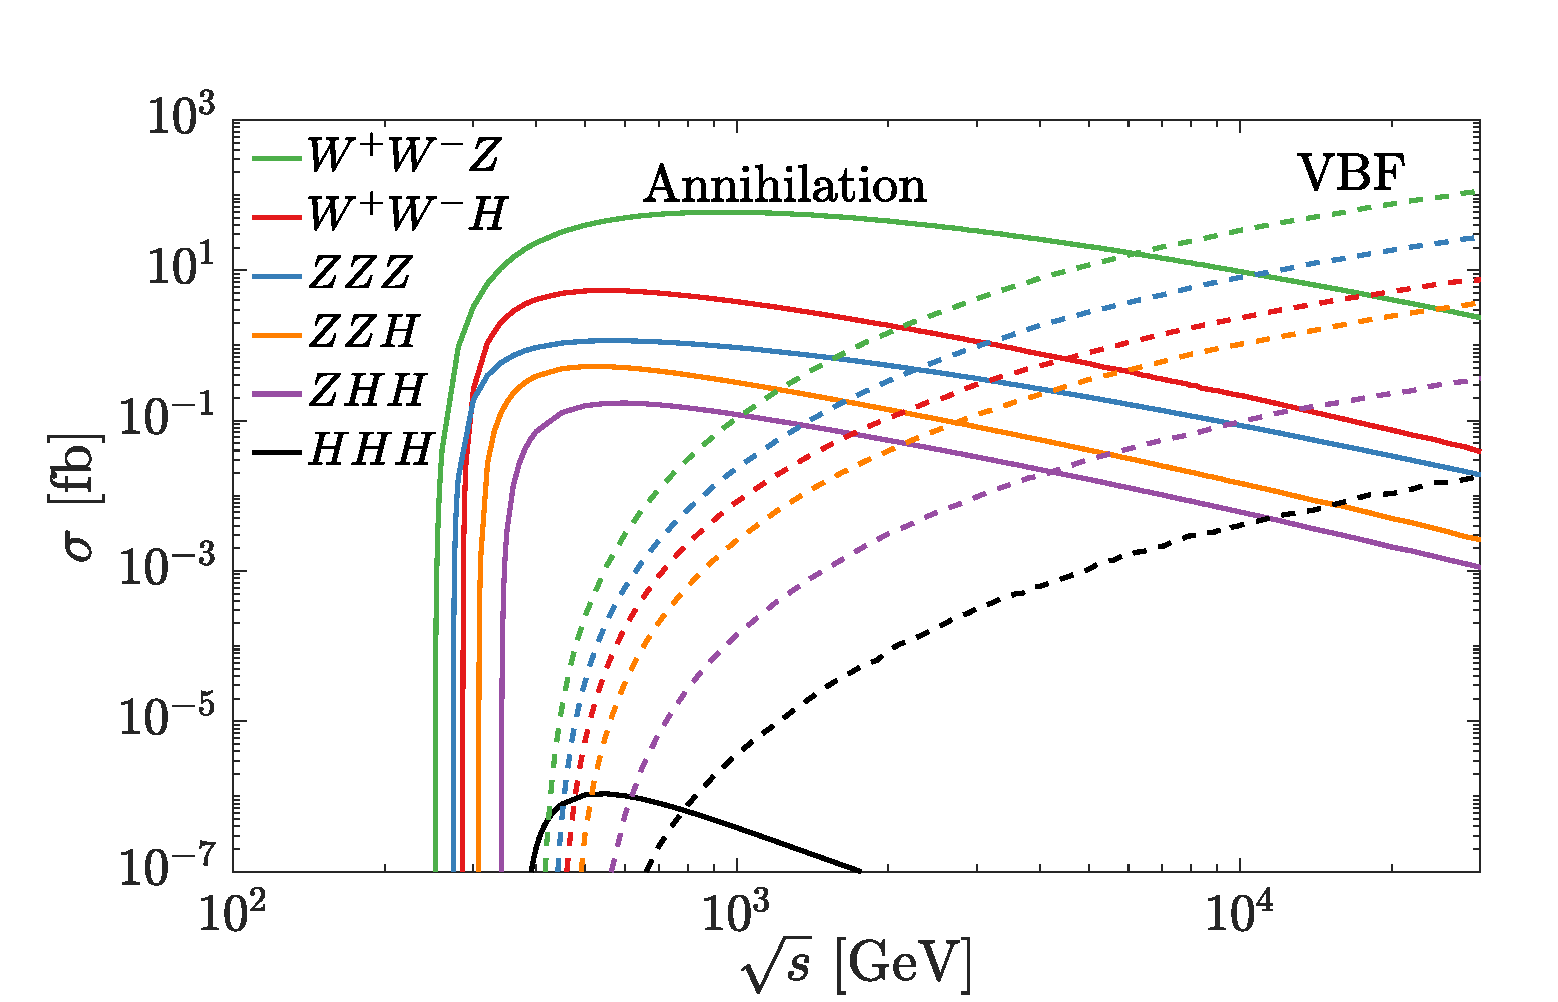
\includegraphics[width=0.48\textwidth]{figs/BBB_SM.pdf}
	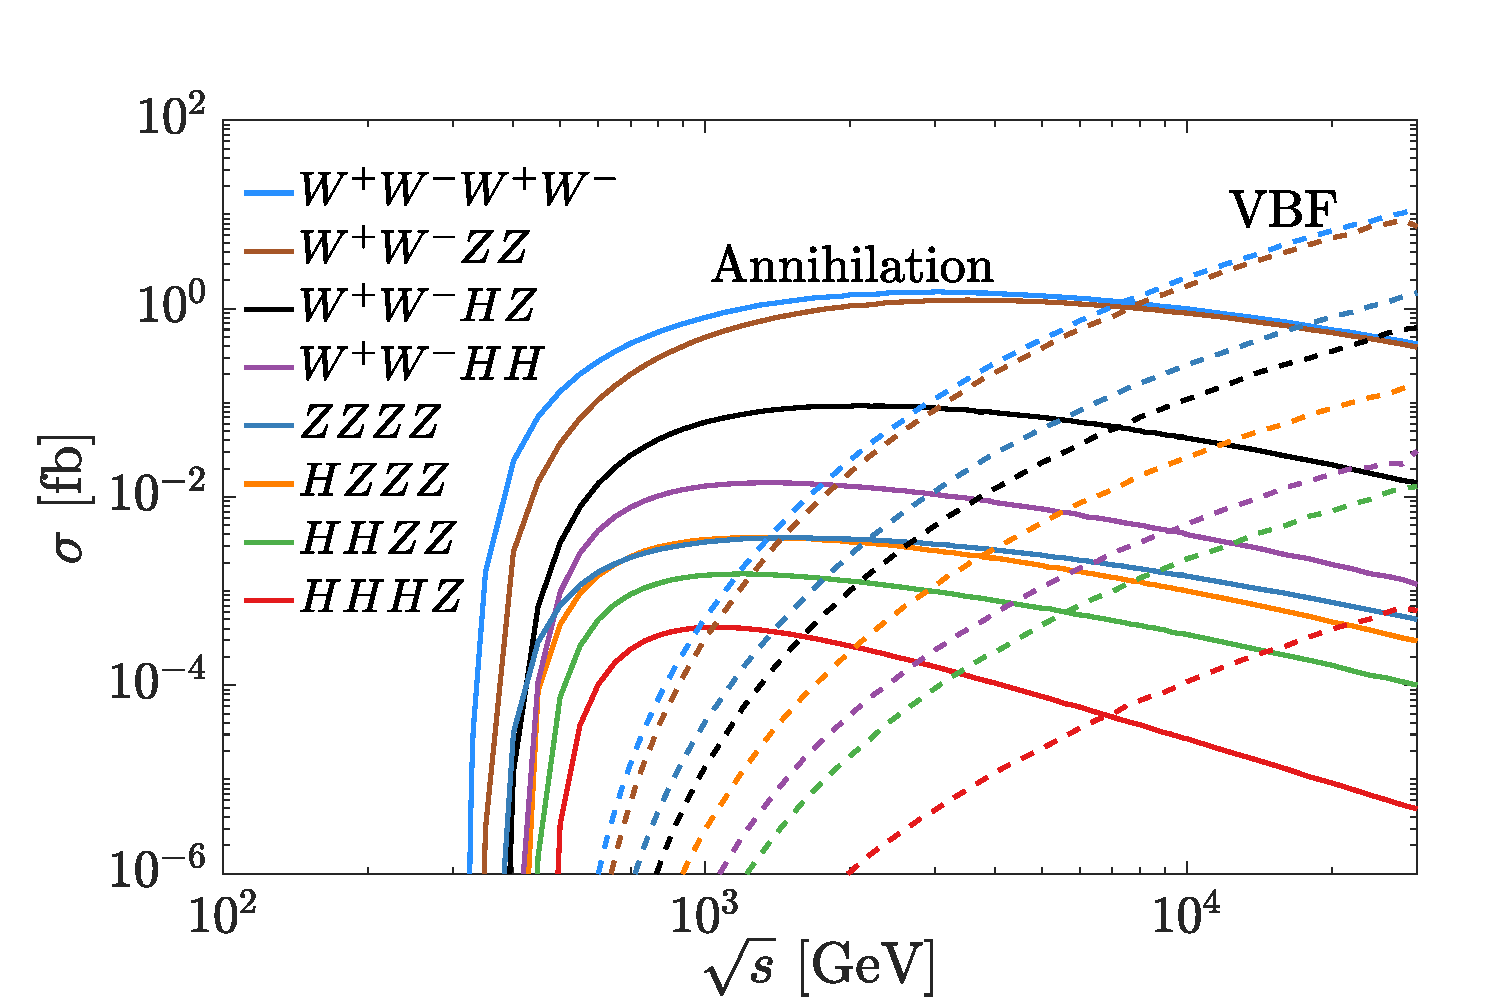
\includegraphics[width=0.46\textwidth]{figs/BBBB_SM.pdf}
	\begin{columns}
		\begin{column}{0.48\textwidth}
			\textcolor{PittRoyal}{\bf VBF:}
			\begin{itemize}
				\item Increases rapidly
				\item Most events are at the threshold
				\item Highly boosted final state (\textcolor{PittRoyal}{forward/backward})
			\end{itemize}
		\end{column}
		\begin{column}{0.48\textwidth}
			\textcolor{PittRoyal}{\bf Annihilation:}
			\begin{itemize}
				\item Decreases slowly
				\item Most events are at the machine energy
				\item One Boson highly off-shell
				\item  Final state in rest frame (\textcolor{PittRoyal}{central})
			\end{itemize}
		\end{column}
	\end{columns}
	\hspace{3mm}\textcolor{PittGold}{\bf Annihilation processes are important for analysis at all energies}
\end{frame}

\subsection{Muon-Higgs coupling}
%%%%%%%%%%%%%%%%%%%%%%%%%%%%%%%%%%%%%%%%%%%%
% Cover: muon Yukawa
%%%%%%%%%%%%%%%%%%%%%%%%%%%%%%%%%%%%%%%%%%%%
\begin{frame}
	\vspace{6mm}
	\centering
	\textcolor{PittRoyal}{{\Huge \bf Muon-Higgs Coupling }}
	\vspace{5mm}
	\begin{itemize}
		\item Physics: We actually do not know whether the SM mass-generation mechanism
		applies just to the heavy particles, or also to the 1st/2nd generations.
		\item Logical possibility: Muon mass not (only) generated by SM Higgs.\\
		$\Rightarrow$ \textcolor{PittRoyal}{\bf Why not have an arbitrary Yukawa coupling?}
	\end{itemize}
\end{frame}

%%%%%%%%%%%%%%%%%%%%%%%%%%%%%%%%%%%%%%%%%%%%
% Two & three -boson final states
%%%%%%%%%%%%%%%%%%%%%%%%%%%%%%%%%%%%%%%%%%%%
\begin{frame}
	\frametitle{Multi-boson final states and the Muon-Higgs coupling}
		\begin{itemize}
			\item \textcolor{PittRoyal}{\bf SM}: $\lambda ({\rm Muon-Higgs})\sim y_\mu^{\rm SM} = \sqrt{2}m_\mu^{\rm SM}/v$
			\item \textcolor{PittRoyal}{\bf Possible BSM physics}: $m_\mu=m_\mu^{\rm SM}$, \textcolor{red}{$\lambda ({\rm Muon-Higgs})\sim \kappa_\mu y_\mu^{\rm SM}$}, e.g. $\kappa_\mu=0$
		\end{itemize}
	\begin{columns}
		\begin{column}{0.5\textwidth}
			\textcolor{black}{\bf Two-boson final states}
		\centering
		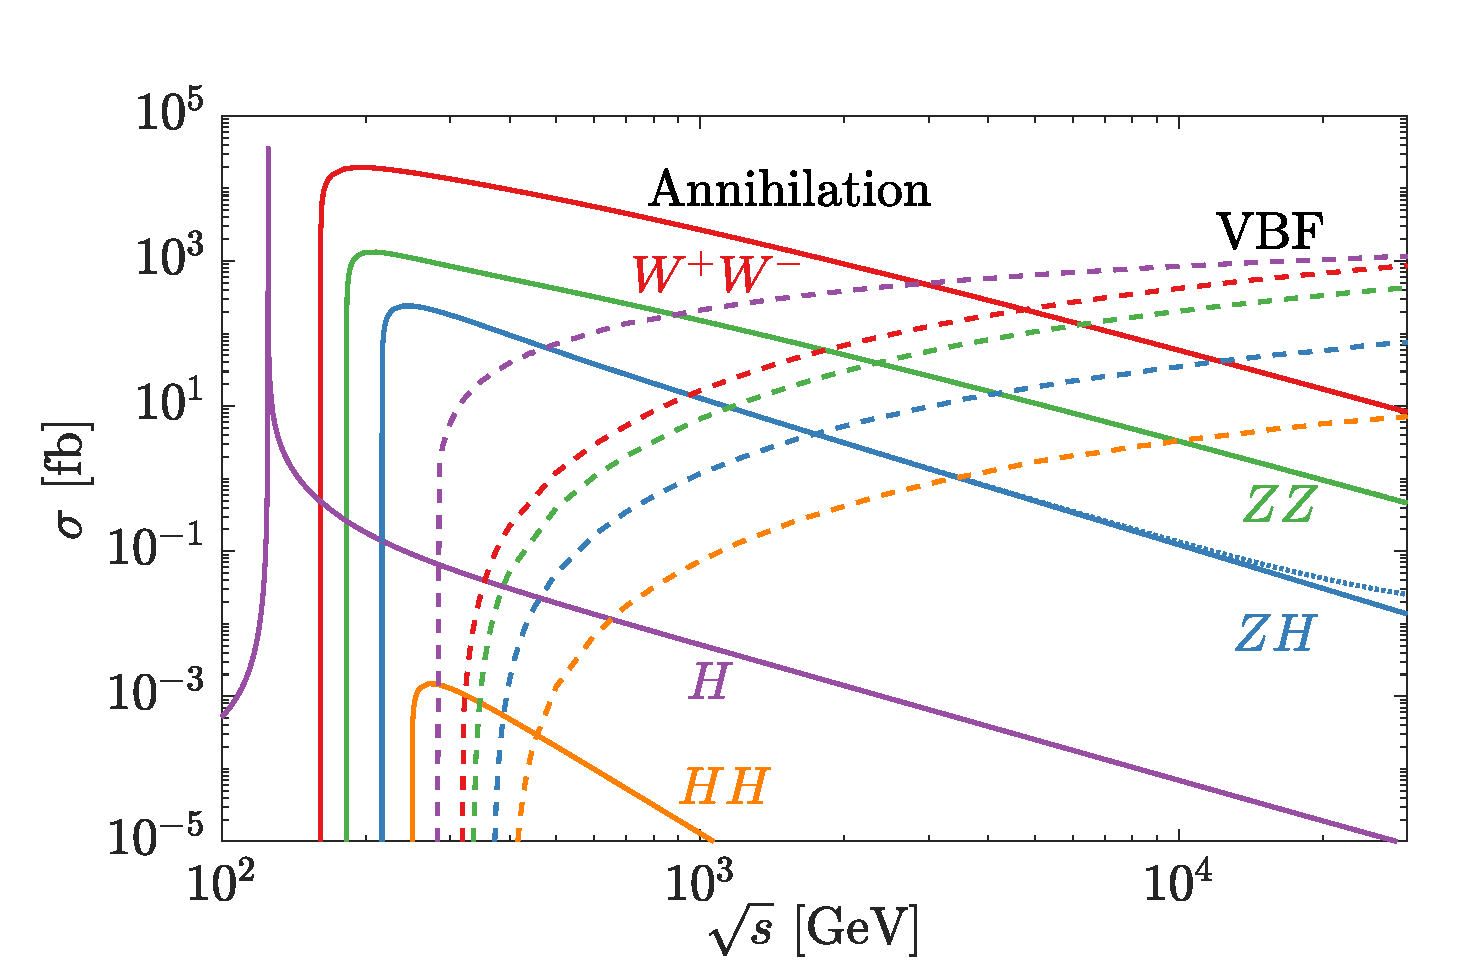
\includegraphics[width=0.88\textwidth]{figs/BB3.pdf}
		\end{column}
		\begin{column}{0.5\textwidth}
			\textcolor{black}{\bf Three-boson final states}
		\centering
		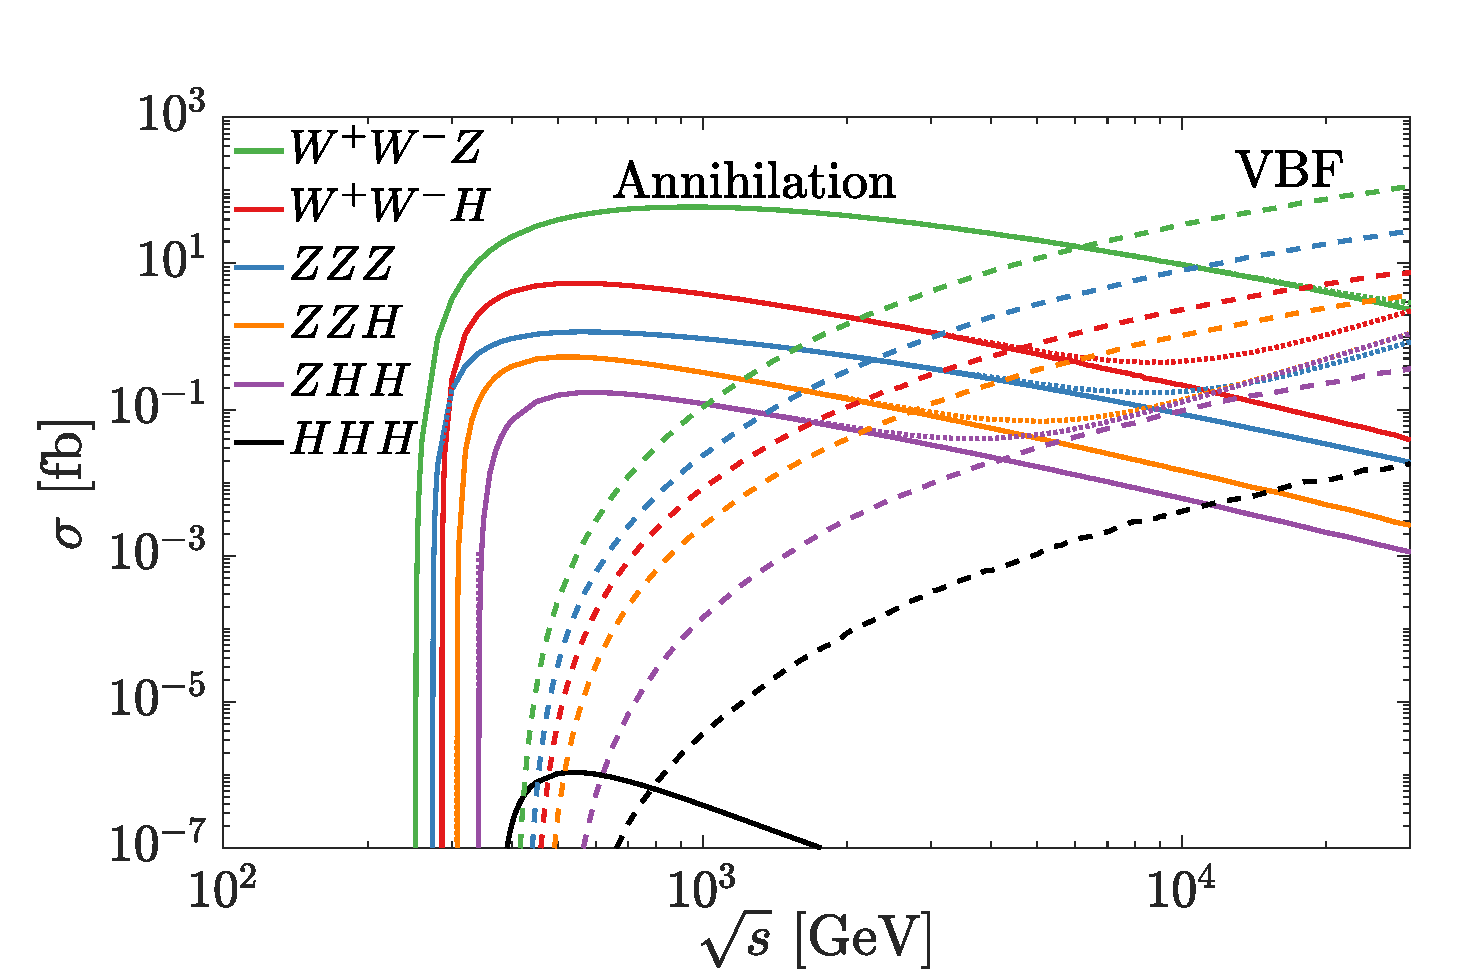
\includegraphics[width=0.88\textwidth]{figs/BBB2.pdf}
		\end{column}
		\end{columns}
	
 \textcolor{red}{\bf  New physics signal shows up in the high energy region}
\end{frame}


%%%%%%%%%%%%%%%%%%%%%%%%%%%%%%%%%%%%%%%%%%%%
% Kinematics: WWH
%%%%%%%%%%%%%%%%%%%%%%%%%%%%%%%%%%%%%%%%%%%%
\begin{frame}
	\frametitle{$WWH$ at a $10$ TeV muon collider: Kinematics}
	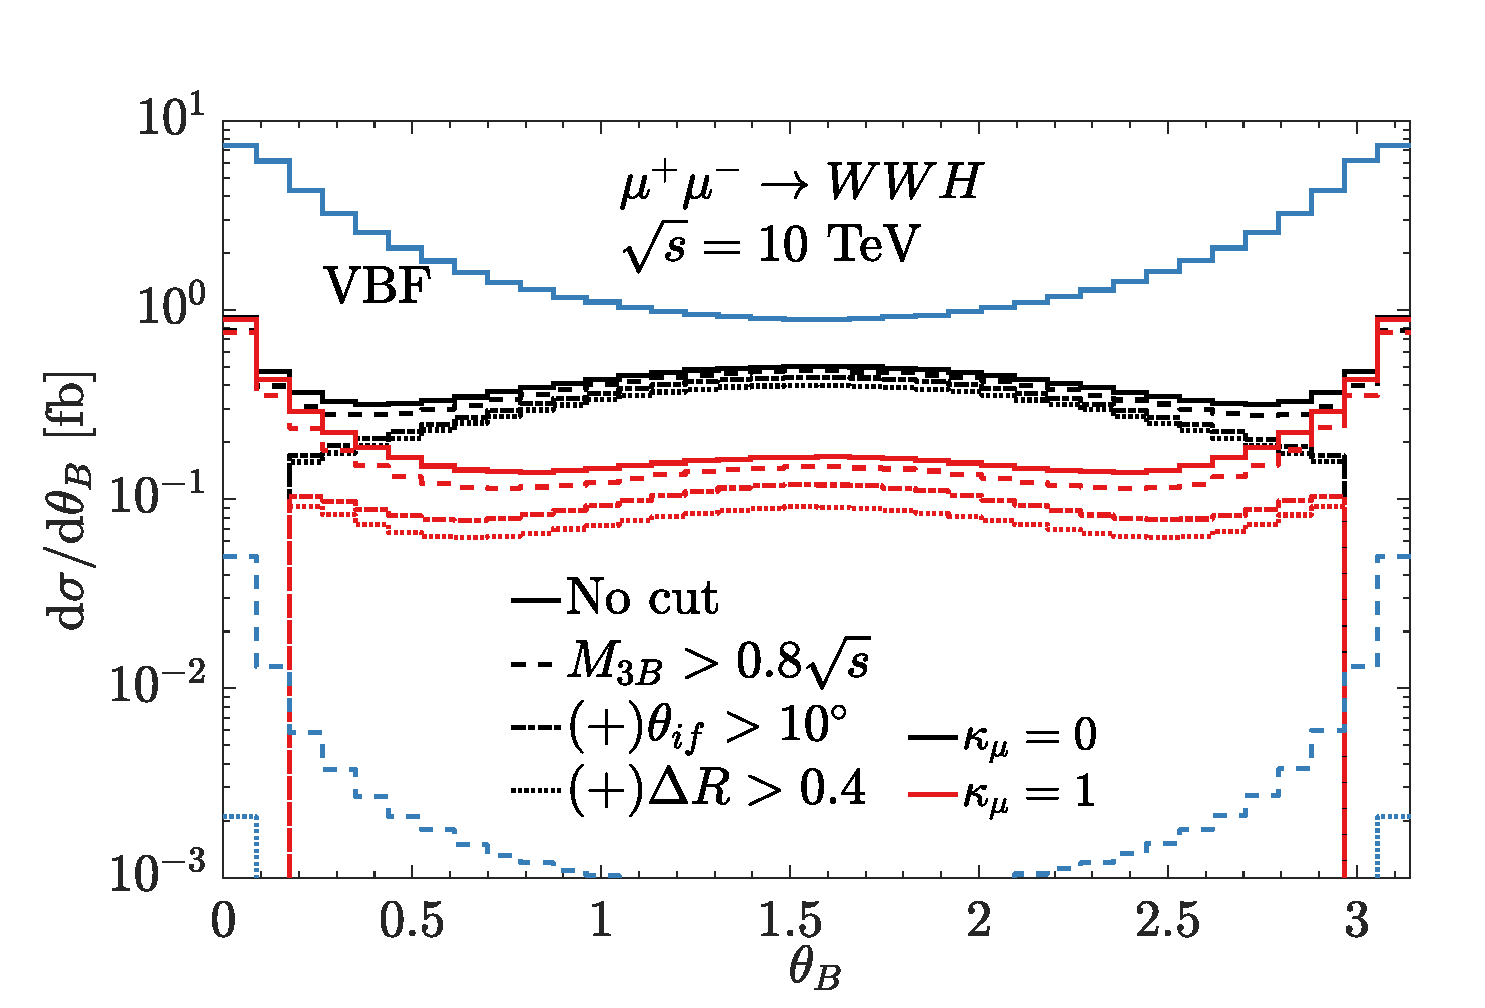
\includegraphics[width=0.33\textwidth]{figs/dist/WWH_ThetaB}
	\includegraphics[width=0.33\textwidth]{figs/dist/WWH_M3B}
	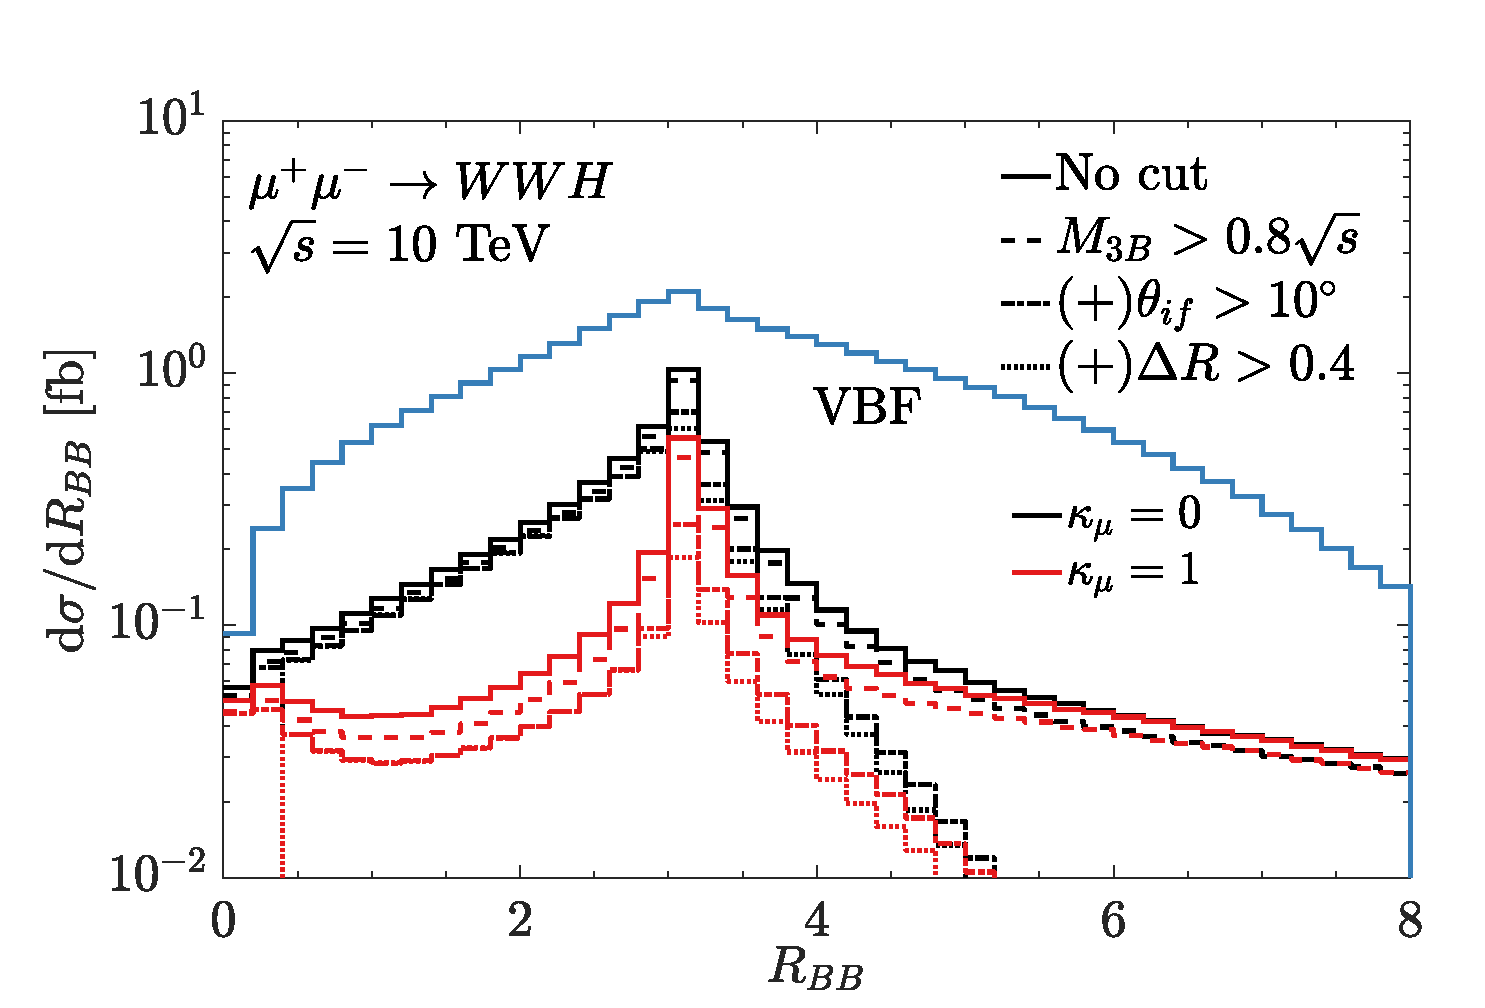
\includegraphics[width=0.33\textwidth]{figs/dist/WWH_RBB}

	\begin{itemize}
	\item {\small Background (VBF) is much larger than signal (annihilation)}
	\item {\small VBF events accumulate around threshold, and mostly forward}
	\item {\small Annihilation in the rest frame (central, and $M\sim\sqrt{s}$ spread by ISR)}
	\item {\small Annihilation also has forward dominance, due to the gauge splitting $W\to WH$}
	\end{itemize}
\end{frame}


%%%%%%%%%%%%%%%%%%%%%%%%%%%%%%%%%%%%%%%%%%%%
% Cuts: WWH
%%%%%%%%%%%%%%%%%%%%%%%%%%%%%%%%%%%%%%%%%%%%
\begin{frame}
	\frametitle{$WWH$ at a $10$ TeV muon collider: Cuts}
	\centering
	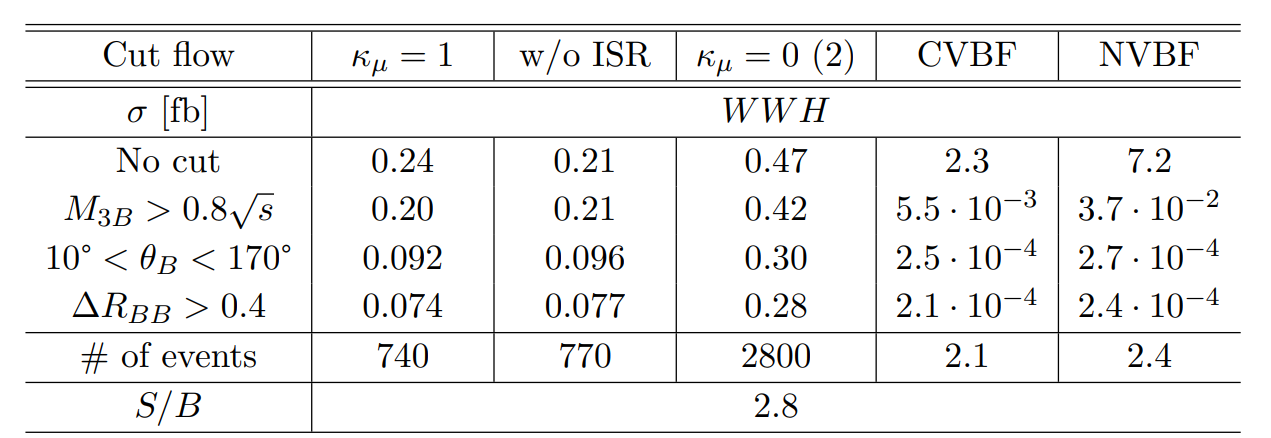
\includegraphics[width=0.8\textwidth]{figs/WWH_cut.png}
	\begin{itemize}
		\item Integrated luminosity $\mathcal{L}=(\sqrt{s}/10~ \TeV )^2\cdot10~\textrm{ab}^{-1}$ \bib{1901.06150}
		\item $S=N_{\kappa_\mu}-N_{\kappa_\mu=1}, ~ B=N_{\kappa_\mu=1}+N_{\rm VBF}$.
		\item VBF and ISR are mostly excluded by invariant mass cut.
		\item Angular cut also weaken VBF further.
	\end{itemize}
\end{frame}

%%%%%%%%%%%%%%%%%%%%%%%%%%%%%%%%%%%%%%%%%%%%
% The statistical sensitivity
%%%%%%%%%%%%%%%%%%%%%%%%%%%%%%%%%%%%%%%%%%%%
\begin{frame}
	\frametitle{Test the muon Yukawa: statistical sensitivity}
	\vspace{3mm}
	\begin{itemize}
		% \item Due to the symmetry $\sigma_{\kappa_\mu=1-\delta}=\sigma_{\kappa_\mu=1+\delta}$, we can only probe the absolute deviation $|\kappa_\mu-1|$, without information about the sign.
		\item The most sensitive channels are $ZHH$ and $ZZH$, similar probes due to GBET.
		\item Taking $S=2$ criterion, we can test the muon-Higgs coupling up to 10\% (1\%) precision at a 10 (30) TeV muon collider, corresponding to new physics scale $\Lambda_{\rm NP}\sim30-100$ TeV.
		\end{itemize}
	% \vspace{-1mm}
	\centering
	\includegraphics[width=0.58\textwidth]{figs/sig_contour}
\end{frame}

%% ===========================================
%% ===========================================
\section{Higgs decay to charmonia and Charm Yukawa} 

%%%%%%%%%%%%%%%%%%%%%%%%%%%%%%%%%%%%%%%%%%%%
% Cover: Charm Yukawa
%%%%%%%%%%%%%%%%%%%%%%%%%%%%%%%%%%%%%%%%%%%%
\begin{frame}
	\vspace{6mm}
	\centering
	\textcolor{PittRoyal}{{\Huge \bf Charm-Higgs Coupling }}\\
	\vspace{5mm}
	\textcolor{red}{\bf \Large The same question is asked again }
	\begin{itemize}
		\item Physics: We actually do not know whether the SM mass-generation mechanism
		applies just to the heavy particles, or also to the 1st/2nd generations.
		\item Logical possibility: Muon mass not (only) generated by SM Higgs.\\
		$\Rightarrow$ \textcolor{PittRoyal}{\bf What if the Charm-Higgs coupling is not related to $m_c$ ?}
	\end{itemize}
\end{frame}


%%%%%%%%%%%%%%%%%%%%%%%%%%%%%%%%%%%%%%%%%%%%
% Current status 
%%%%%%%%%%%%%%%%%%%%%%%%%%%%%%%%%%%%%%%%%%%%
\begin{frame}{Current status of charm Yukawa coupling testing}
	\hspace{3mm}\textcolor{PittRoyal}{\bf Measuring $Hc{\bar c}$ coupling is not easy}
\begin{itemize}
	\item Branching fraction ($H \to c {\bar c}$): $2.9\%$
	\item Large QCD background at hadron colliders
	\item $c$-tagging is challenging
\end{itemize}

\vspace{2mm}
\hspace{3mm}\textcolor{PittRoyal}{\bf Current experimental searching}
\begin{itemize}
	\item $\kappa$ framework: For $y_c^{\rm SM} = \sqrt{2}m_c/v$, set $y_c=\kappa_c y_c^{\rm SM}$
	\item $pp\to VH (c{\bar c}) $
	\begin{itemize}
		\item \textcolor{red}{Need c-tagging}.
		\item LHC Run 2: ATLAS $\kappa_c \leq 8.5$ \bib{ATLAS-CONF-2021-021}, \textcolor{red}{CMS $1.1< |\kappa_c| < 5.5$} \bib{CMS-PAS-HIG-21-008}  
		\item Future HL-LHC: $\kappa_c \leq 3$. \bib{2201.11428, ATL-PHYS-PUB-2021-039}
	\end{itemize}
	\item Production of $c{\bar c}$ bound states via Higgs decay: $H\to J/\psi +\gamma$
	\begin{itemize}
		\item Clean final states $J/\psi \to \mu^+ \mu^-$, avoid c-tagging
		\item The rate is too low: $BR\sim 10^{-6}$. \bib{1306.5770, 1407.6695}
		\item Result is less sensitive: $\kappa_c \leq 100$. \bib{1807.00802, 1810.10056}
	\end{itemize}
\end{itemize}
\end{frame}

\subsection{Non-relatisvistic QCD calculation formalism}
%%%%%%%%%%%%%%%%%%%%%%%%%%%%%%%%%%%%%%%%%%%%
% NRQCD
%%%%%%%%%%%%%%%%%%%%%%%%%%%%%%%%%%%%%%%%%%%%
\begin{frame}{Our idea: Higgs decay to charmonium in NRQCD }
	\vspace{-3mm}

	\begin{columns}
		\begin{column}{0.58\textwidth}
			\begin{small}
				\begin{eqnarray}
					H \to c  + \bar{c} + J/\psi\ ({\rm or}\ \eta_c)\nonumber
				\end{eqnarray}
				\end{small}
	\hspace{3mm}\textcolor{PittRoyal}{\bf Nonrelativistic QCD framework}
	\begin{tiny}
	\begin{eqnarray}
		&&\Gamma =\sum_\mathbb{N}  {\hat \Gamma}_\mathbb{N}(H \to(Q {\bar Q})[\mathbb{N}]+X)\times \langle {\cal O}^h[\mathbb{N}] \rangle,\nonumber \\ 
		&&\dd {\hat \Gamma}_\mathbb{N}=\frac{1}{2 m_H}\frac{|{\cal M}|^2}{\langle {\cal O}^{Q{\bar Q}}\rangle} \dd \Phi_3\nonumber
	\end{eqnarray}
	\end{tiny}
	\hspace{5mm}\textcolor{PittRoyal}{\bf Long distance matrix element (LDME)}\\
	\hspace{7mm}Related to the wave function at origin
	\begin{tiny}
	\begin{eqnarray}
		&&\langle {\cal O}^{J/\psi}[^3S_1^{[1]}] \rangle =\frac{3 N_c}{2\pi} |R(0)|^2, ~~ \langle {\cal O}^{\eta_c}[^1S_0^{[1]}] \rangle= \frac{N_c}{2\pi} |R(0)|^2,~~\nonumber \\ &&\langle {\cal O}^{Q{\bar Q}}\rangle =6 N_c ,\  {\text {\rm for }} ^3S_1^{[1]}, ~~
        \langle {\cal O}^{Q{\bar Q}}\rangle =2 N_c ,\  {\text {\rm for }} ^1S_0^{[1]} \nonumber 
	\end{eqnarray}
	\end{tiny}
\end{column}
\hspace*{-5mm}
\begin{column}{0.4\textwidth}
	\textcolor{PittRoyal}{Color-singlet}: \\
	Charm quark fragmentation to $^3S_1^{[1]}(J/\psi)$ and $^1S_0^{[1]}(\eta_c)$
	\begin{center}
		\includegraphics[width=.45\textwidth]{figs/Feynman_hcc_COCS_QCDQED1.pdf}
		\includegraphics[width=.45\textwidth]{figs/Feynman_hcc_COCS_QCDQED2.pdf}
		\includegraphics[width=.45\textwidth]{figs/Feynman_hcc_COCS_QCDQED3.pdf}
		\includegraphics[width=.45\textwidth]{figs/Feynman_hcc_COCS_QCDQED4.pdf}
	\end{center}
\end{column}
\end{columns}

\end{frame}


%%%%%%%%%%%%%%%%%%%%%%%%%%%%%%%%%%%%%%%%%%%%
% QED/EW corrections
%%%%%%%%%%%%%%%%%%%%%%%%%%%%%%%%%%%%%%%%%%%%
\begin{frame}{More corrections from QED and EW sector}
	\hspace{3mm}\textcolor{PittRoyal}{\bf Pure QED diagrams: sizable correction to $^3S_1^{[1]}(J/\psi)$ production}\\
	\hspace{5mm}\vspace{1mm}Single photon fragmentation (SPF) $\Rightarrow$ {\bf logarithmic enhancement} \\
	\begin{center}
    \includegraphics[width=.2\textwidth]{figs/Feynman_hcc_CS_QED1.pdf}
    \includegraphics[width=.2\textwidth]{figs/Feynman_hcc_CS_QED2.pdf}
    \includegraphics[width=.2\textwidth]{figs/Feynman_hcc_CS_QED3.pdf}
    \includegraphics[width=.2\textwidth]{figs/Feynman_hcc_CS_QED4.pdf}
	\end{center}
	\hspace{3mm}\textcolor{PittRoyal}{\bf Electroweak correction from the $HZZ$ diagrams}\\
	\hspace{5mm}\vspace{1mm}One of the $Z$ can be on shell $\Rightarrow$ {\bf resonance enhancement}
	\begin{center}
		\includegraphics[width=.22\textwidth]{figs/Feynman_hzz_cc1.pdf}
		\includegraphics[width=.22\textwidth]{figs/Feynman_hzz_cc2.pdf}
	\end{center}
	\hspace{10mm}\vspace{1mm} \small{$\bullet$ Sizable for $^1S_0^{[1]}(\eta_c)$ due to the larger axial $Zc\bar{c}$ coupling.}
\end{frame}


%%%%%%%%%%%%%%%%%%%%%%%%%%%%%%%%%%%%%%%%%%%%
% Cplor octet 
%%%%%%%%%%%%%%%%%%%%%%%%%%%%%%%%%%%%%%%%%%%%
\begin{frame}{Charmonium productiuon via color octet states}
	\hspace{3mm}\textcolor{PittRoyal}{\bf A key property of NRQCD}\\
	\begin{itemize}
		\item A quarkonium can also be produced through {\bf color-octet} $Q{\bar Q}$ Fork states
		\item New states involved: $^3S_1^{[8]}$, $^1S_0^{[8]}$, $^3P_J^{[8]}$, and $^1P_1^{[8]}$
		\item The LDMEs $\langle {\cal O}^h[^{2S+1}L_J^{\rm [color]}] \rangle$ need to be fitted from experimental data
	\end{itemize}

	\begin{table}[htb]
		\scalebox{0.7}{
		\begin{tabular}{lccc}
		\hline
		Reference            & $\langle {\cal O}^{J/\psi}[^1S_0^{[8]}] \rangle$ & $\langle {\cal O}^{J/\psi}[^3S_1^{[8]}] \rangle$ & $\langle {\cal O}^{J/\psi}[^3P_0^{[8]}] \rangle/m_c^2$ \\ \hline
		G. Bodwin,        & $(9.9\pm2.2)\times10^{-2}$                       & $(1.1\pm1.0)\times10^{-2}$                      & $(4.89\pm4.44)\times 10^{-3}$                           \\
		K.T. Chao,      & $(8.9\pm0.98)\times10^{-2}$                      & $(3.0\pm1.2)\times 10^{-3}$                      & $(5.6\pm2.1)\times 10^{-3}$                            \\
		Y. Feng,       & $(5.66\pm4.7)\times 10^{-2}$                     & $(1.77\pm0.58)\times 10^{-3}$                    & $(3.42\pm1.02)\times 10^{-3}$                          \\ \hline
		\end{tabular}
		}
	\end{table}

	\hspace{3mm}\textcolor{PittRoyal}{\bf New diagrams for $^3S_1^{[8]}$}\\
	\hspace{5mm}Single gluon fragmentation (SGF)  $\Rightarrow$ {\bf logarithmic enhancement}
	\begin{center}
		\includegraphics[width=.22\textwidth]{figs/Feynman_hcc_CO_QCD1.pdf}
		\includegraphics[width=.22\textwidth]{figs/Feynman_hcc_CO_QCD2.pdf}
		\includegraphics[width=.22\textwidth]{figs/Feynman_hcc_CO_QCD3.pdf}
		\includegraphics[width=.22\textwidth]{figs/Feynman_hcc_CO_QCD4.pdf}
	\end{center}
\end{frame}

\subsection{The Standard Model results}
%%%%%%%%%%%%%%%%%%%%%%%%%%%%%%%%%%%%%%%%%%%%
% SM results
%%%%%%%%%%%%%%%%%%%%%%%%%%%%%%%%%%%%%%%%%%%%
\begin{frame}{Standard Model results (I)}
	\hspace{3mm}\textcolor{PittRoyal}{\bf Numerical parameters}
	\begin{tiny}
	\begin{eqnarray}
		&&\alpha=1/132.5, ~~\alpha_s(2 m_c)=0.235,~~ m_c^{\rm pole}=1.5~{\rm GeV},
		~~m_c(m_H)=0.694~{\text {\rm GeV}}, ~~
			m_H=125~{\text {\rm GeV}}, \nonumber \\
			&&m_W=80.419~{\text {\rm GeV}},~~ m_Z=91.188~{\text {\rm GeV}},
			~~v =246.22\ {\text {\rm GeV}},~~y_c^{\rm SM}= \frac{{\sqrt 2}m_c(m_H)}{ v} \approx 3.986\times 10^{-3}. \nonumber
	\end{eqnarray}
	\end{tiny}
	\vspace{-2mm}\hspace{3mm}\textcolor{PittRoyal}{\bf Decay width and branching fraction}
	\begin{table}[htb]
		\scalebox{0.62}{
			\begin{tabular}{lccccc}
				\hline
				\multicolumn{1}{c}{}                   & QCD [CS]              & QCD+QED [CS]          & Full [CS]             & Full [CO]             & Full [CS+CO]          \\ \hline
				$\Gamma(H\to c{\bar c}+J/\psi)$ (GeV) & $4.8\times 10^{-8}$ & $5.8\times 10^{-8}$ & $6.1\times 10^{-8}$ & $2.2\times 10^{-8}$ & $8.3\times 10^{-8}$ \\
				${\rm BR}(H\to c{\bar c}+J/\psi)$     & $1.2\times 10^{-5}$ & $1.4\times 10^{-5}$ & $1.5\times 10^{-5}$ & $5.3\times 10^{-6}$ & $2.0\times 10^{-5}$ \\
				\hline
				$\Gamma(H\to c{\bar c}+\eta_c)$ (GeV) & $4.9\times 10^{-8}$ & $5.1\times 10^{-8}$ & $6.3\times 10^{-8}$ & $1.8\times 10^{-7}$ & $2.4\times 10^{-7}$ \\
				${\rm BR}(H\to c{\bar c}+\eta_c)$     & $1.2\times 10^{-5}$ & $1.2\times 10^{-5}$ & $1.5\times 10^{-5}$ & $4.5\times 10^{-5}$ & $6.0\times 10^{-5}$ \\ \hline
			\end{tabular}
		}
	\end{table}
	\hspace{3mm}\textcolor{PittRoyal}{\bf Charmonium energy distributions}
	\vspace{-2mm}
	\begin{center}
		\includegraphics[width=.4\textwidth]{figs/dGmdEJpsiSM_Norm.pdf}
		\includegraphics[width=.4\textwidth]{figs/dGmdEetaSM_Norm.pdf}
	\end{center}
\end{frame}

%%%%%%%%%%%%%%%%%%%%%%%%%%%%%%%%%%%%%%%%%%%%
% PT distribution
%%%%%%%%%%%%%%%%%%%%%%%%%%%%%%%%%%%%%%%%%%%%
\begin{frame}{Standard Model results (II): Transverse momentum ($p_T$) distributions}
	\begin{columns}
	\begin{column}{0.5\textwidth}
	\begin{center}
		\vspace{-1mm}\hspace{3mm}\textcolor{black}{\bf Charmonium $p_T$ distributions}
		\includegraphics[width=.75\textwidth]{figs/dGmdhptJPSM_Norm.pdf}
		\includegraphics[width=.75\textwidth]{figs/dGmdhptetaSM_Norm.pdf}
	\end{center}
	\end{column}
	\vspace{-1mm}
	\begin{column}{0.5\textwidth}
		\begin{center}
			\vspace{-1mm}\hspace{3mm}\textcolor{black}{\bf Free charm quark $p_T$ distributions}
			\includegraphics[width=.75\textwidth]{figs/dGmdcptJPSM_Norm.pdf}
		\includegraphics[width=.75\textwidth]{figs/dGmdcptetaSM_Norm.pdf}
		\end{center}
	\end{column}
\end{columns}
\end{frame}

\subsection{Probe the Charm-Higgs coupling}
%%%%%%%%%%%%%%%%%%%%%%%%%%%%%%%%%%%%%%%%%%%%
% Probe the charm Yukawa 
%%%%%%%%%%%%%%%%%%%%%%%%%%%%%%%%%%%%%%%%%%%%
\begin{frame}{Probe the $Hc{\bar c}$ coupling (I)}
	\vspace{3mm}\hspace{3mm}\textcolor{black}{\bf Use the $\kappa$ framework $y_c=\kappa_c y_c^{\rm SM},~{\rm BR} \approx \kappa_c^2\ {\rm BR}^{\rm SM}$}
	\begin{center}
		\includegraphics[width=.68\textwidth]{figs/BR_ratio.pdf}
	\end{center}
\end{frame}

%%%%%%%%%%%%%%%%%%%%%%%%%%%%%%%%%%%%%%%%%%%%
% Discussions  
%%%%%%%%%%%%%%%%%%%%%%%%%%%%%%%%%%%%%%%%%%%%
\begin{frame}{Probe the $Hc{\bar c}$ coupling (II)}
	\hspace{3mm}\textcolor{PittRoyal}{\bf Some rough analysis}:
	\begin{itemize}
		\item Higgs production cross section at LHC $\sigma_H\sim 50~$pb
		\item Expect HL-LHC $L\sim 3~{\rm ab}^{-1}$ at ATLAS and CMS and $L\sim 0.3~{\rm ab}^{-1}$ at LHCb
		\item Detection efficiency $\epsilon$ for the final state $c\bar{c} +\ell^+\ell^-$
		\item ${\rm BR}(J/\psi\to\ell^+\ell^-)\sim 12\%$, ${\rm BR}(H\to J/\psi+c\bar{c})\sim 2\times 10^{-5}$
		\item Event number
		\begin{eqnarray}
			N = L \sigma_H^{}\ \epsilon\ {\rm BR}(H\to J/\psi+c\bar{c}) {\rm BR}(J/\psi\to\ell^+\ell^-) \approx 24\ \kappa_c^2 \times {L\over {\rm ab}^{-1}}\times {\epsilon \over 20\%}\nonumber
		\end{eqnarray}
		\item Considering the statistical error only $\delta N\sim \sqrt{N}$ gives
		\begin{eqnarray}
			\Delta\kappa_c \approx 10\% \times ({L\over {\rm ab}^{-1}}\times {\epsilon \over 20\%})^{-1/2} \nonumber
		\end{eqnarray}
	\end{itemize}
	\vspace{3mm}\hspace{5mm}\textcolor{PittRoyal}{\bf $\bullet$ With $\epsilon\sim 20\%$, we see $\Delta \kappa_c \sim 6\%$ at ATLAS and CMS.}\\
	\vspace{2mm}\hspace{5mm}\textcolor{PittRoyal}{\bf $\bullet$ For a smaller luminosity, $\Delta \kappa_c \sim 18\%$ at LHCb.}
\end{frame}


%% ===========================================
%% ===========================================
\section{Conclusion}
%% ===========================================
%%%%%%%%%%%%%%%%%%%%%%%%%%%%%%%%%%%%%%%%%%%%
% Summary 
%%%%%%%%%%%%%%%%%%%%%%%%%%%%%%%%%%%%%%%%%%%%
\begin{frame}
	\frametitle{Conclusion}
	\begin{itemize}
		% \item The Standard Model of particle physics is one of the most successful achievements in modern physics, however more work need to de done at future high-energy colliders. 
		\item At very high energies, the collinear splittings dominate. {\bf All SM particles should be treated as partons that described by proper PDFs.}
		\begin{itemize}
			\item The large collinear logarithm needs to be resummed via solving the DGLAP equations, so the {\bf QCD partons (quarks and gluons) emerge}.
			\item When $Q>M_Z$, the EW splittings are activated: the EW partons appear, and the existing QED$\otimes$QCD PDFs may receive big corrections.
		\end{itemize}
		\item A high-energy lepton collider is an EW version of HE LHC. We have laid out the EW PDFs framework and provide the SM expectation for future leoton colliders.
		\item Higgs is believed to be a portal to the new physics beyond the SM. 
		\begin{itemize}
			\item By using multi-boson production processes, we claim that it is possible to measure Muon-Higgs coupling to $10\%$ level at future 10-TeV level muon collider.
			\item We also suggest to test the charm-Higgs coupling using Higgs decay to charmonia process at the HL-LHC.
		\end{itemize}
	\end{itemize}

	

\end{frame}

%% ===========================================
%% ===========================================

\begin{frame}{Acknowledgement}
\Background
\vspace{-4mm}{\LARGE \centerline{Thanks !}}
\vspace{-3mm}
\begin{itemize}
	\item To the committee members:\\
	Tao Han, Brian Batell, Vittorio Paolone, Manfred Paulini, Andrew Zentner
	\item To those who were teaching me in the past $6$ years:\\
	Tao Han, Brian Batell, Daniel Boyanovsky, Ayres Freitas, Kaoru Hagiwara, Jeremy Levy, Roger Mong, Manfred Paulini, Andrew Zentner
	\item To my collaborators: \\
	Tao Han, Adam Leibovich, Keping Xie, Wolfgang Kilian, Nils Kreher, Jürgen Reuter,...
	\item To my colleagues and classmates:\\
	Rudrajit Banerjee, Hongbo Cai, Lisong Chen, Yilun Guan, Sze Ching Leung, Chi Wing Ng, Qian Song, Barmak Shams Es Haghi, Yongcheng Wu, Zhite Yu, Bomin Zhang, ...
	\item To Prof. Stanley Brodsky for ``Yang, you should work hard''
\end{itemize}
\textcolor{black}{\bf \Large I will continue working hard at} {\bf \Large \textcolor{INFNBlue1}{IN}\textcolor{INFNBlue2}{F}\textcolor{INFNBlue1}{N} \textcolor{INFNBlue2}{Bologna}}
\end{frame}


%% ===========================================
%% ===========================================
\appendix
\section{The full SM DGLAP}
%%%%%%%%%%%%%%%%%%%%%%%%%%%%%%%%%%%%%%%%%%%%
% Singlet and Non-singlet
%%%%%%%%%%%%%%%%%%%%%%%%%%%%%%%%%%%%%%%%%%%%
\begin{frame}{Solving the DGLAP: Singlet and Non-singlet PDFs}
	The singlets
	\beq\nonumber
	f_L=\sum_{i=e,\mu,\tau}(f_{\ell_i}+f_{\bar{\ell}_i}), ~ 
	f_U=\sum_{i=u,c}(f_{u_i}+f_{\bar{u}_i}), ~ 
	f_D=\sum_{i=d,s,b}(f_{d_i}+f_{\bar{d}_i})
	\eeq
	The non-singlets
	\begin{itemize}
		\item The only non-trivial singlet ~~~$f_{e,NS}=f_{e}-f_{\bar{e}}$
		\item the leptons ~~~ $f_{\ell_i,NS}=f_{\ell_i}-f_{\bar{\ell}_i}(i=2,3), ~f_{\ell,12}=f_{\bar{e}}-f_{\bar{\mu}}, ~f_{\ell,13}=f_{\bar{e}}-f_{\bar{\tau}}$;
		\item 
		the up-type quarks ~~~$f_{u_i,NS}=f_{u_i}-f_{\bar{u}_i}, ~f_{u,12}=f_u-f_c$;
		\item 
		and the down-type quarks ~~~$f_{d_i,NS}=f_{d_i}-f_{\bar{d}_i}, ~ f_{d,12}=f_{d}-f_{s}, ~ f_{d,13}=f_{d}-f_{b}$.
	\end{itemize}
	Reconstruction:
	\begin{small}
	\begin{equation}\nonumber
	f_{e}=\frac{f_{L}+(2N_{\ell}-1)f_{e,NS}}{2N_{\ell}},~
	f_{\bar{e}}=f_{\mu}=f_{\bar{\mu}}=f_{\tau}=f_{\bar{\tau}}=\frac{f_L-f_{e,NS}}{2N_{\ell}}.
	\end{equation}
	\begin{equation}\nonumber
	f_{u}=f_{\bar{u}}=f_{c}=f_{\bar{c}}=\frac{f_{U}}{2N_u}, ~ f_{d}=f_{\bar{d}}=f_{s}=f_{\bar{s}}=f_{b}=f_{\bar{b}}=\frac{f_{D}}{2N_d}.
	\end{equation}
	\end{small}
\end{frame}


%%%%%%%%%%%%%%%%%%%%%%%%%%%%%%%%%%%%%%%%%%%%
% DGLAP for QED X QCD
%%%%%%%%%%%%%%%%%%%%%%%%%%%%%%%%%%%%%%%%%%%%
\begin{frame}{The QED$\otimes$QCD case}
	% \vspace{2mm}\textcolor{PittRoyal}{\bf The DGLAP reads: }
	\begin{itemize}
	\item The singlets and gauge bosons 
	\begin{small}
	\begin{equation}\nonumber
		\frac{\dd}{\dd \log Q^2}
	\begin{pmatrix}
	f_L\\
	f_U\\
	f_D\\
	f_\gamma\\
	f_g
	\end{pmatrix}=
	\begin{pmatrix}
	P_{\ell\ell} & 0 & 0 & 2N_\ell P_{\ell\gamma} & 0\\
	0 & P_{uu} & 0 & 2N_uP_{u\gamma} & 2N_uP_{ug}\\
	0 & 0 & P_{dd} & 2N_dP_{d\gamma} & 2N_dP_{dg}\\
	P_{\gamma\ell} & P_{\gamma u} &  P_{\gamma d} & P_{\gamma\gamma} & 0\\
	0 & P_{g u} & P_{gd} & 0 & P_{gg}
	\end{pmatrix}
	\otimes 
	\begin{pmatrix}
	f_L\\
	f_U\\
	f_D\\
	f_\gamma\\
	f_g
	\end{pmatrix}
	\end{equation}
	\end{small}	
	\item The non-singlets
	\begin{equation}\nonumber
		\frac{\dd}{\dd \log Q^2} f_{NS}=P_{ff}\otimes f_{NS}.
	\end{equation}
	\item The averaged momentum fractions of the PDFs: $f_{\ell_{\rm val}},\, f_\gamma,\, f_{\ell_{\rm sea}},\, f_q,\, f_g$
	\begin{small}
	\begin{eqnarray}
		\langle x_i\rangle=\int xf_i(x)\dd x,~\sum_i \langle x_i\rangle=1 \nonumber
	\end{eqnarray}
	\vspace{-3mm}
	\begin{eqnarray}
		\frac{\langle x_q\rangle}{\langle x_{\lsea}\rangle}\lesssim \frac{N_c\left[\sum_i(e_{u_i}^2+e_{\bar{u}_i}^2)+\sum_{i}(e_{d_i}^2+e_{\bar{d}_i}^2)\right]}{e^2_{{\bar \ell}_{\rm val}}+\sum_{i\neq\lval}(e_{\ell_i}^2+e_{\bar{\ell}_i}^2)}=\frac{22/3}{5}\nonumber
	\end{eqnarray}
	\end{small}
	\end{itemize}
\end{frame}

%%%%%%%%%%%%%%%%%%%%%%%%%%%%%%%%%%%%%%%%%%%%
% EW DGLAP
%%%%%%%%%%%%%%%%%%%%%%%%%%%%%%%%%%%%%%%%%%%%
\begin{frame}{The DGLAP for the full SM}
	\vspace{-3mm}\begin{small}
	\begin{equation}\nonumber
	\ddL\begin{pmatrix}
	f_{L}^{0\pm}\\
	f_{Q}^{0\pm}\\
	f_{E}^{0\pm}\\
	f_{U}^{0\pm}\\
	f_{D}^{0\pm}\\
	f_{B}^{0\pm}\\
	f_{W}^{0\pm}\\
	f_{g}^{0\pm}
	\end{pmatrix}=
	\begin{pmatrix}
	P_{LL}^{0\pm} & 0 & 0 & 0 & 0 & P_{LB}^{0\pm} & P_{LW}^{0\pm} & 0 \\
	0 &  P_{QQ}^{0\pm} & 0 & 0 & 0 & P_{QB}^{0\pm} & P_{QW}^{0\pm} & P_{Qg}^{0\pm} \\
	0 & 0 & P_{EE}^{0\pm} & 0 & 0 & P_{EB}^{0\pm} & 0 & 0 \\
	0 & 0 & 0 & P_{UU}^{0\pm} & 0 & P_{UB}^{0\pm} & 0 & P_{Ug}^{0\pm} \\
	0 & 0 & 0 & 0 & P_{DD}^{0\pm} & P_{DB}^{0\pm} & 0 & P_{Dg}^{0\pm} \\
	P_{BL}^{0\pm} & P_{BQ}^{0\pm} & P_{BE}^{0\pm} & P_{BU}^{0\pm} & P_{BD}^{0\pm} & P_{BB}^{0\pm} & 0 & 0 \\
	P_{WL}^{0\pm} & P_{WQ}^{0\pm} & 0 & 0 & 0 & 0 & P_{WW}^{0\pm} & 0 \\
	0 & P_{gQ}^{0\pm} & 0 & P_{gU}^{0\pm} & P_{gD}^{0\pm} & 0 & 0 & P_{gg}^{0\pm} \\
	\end{pmatrix}
	\otimes
	\begin{pmatrix}
	f_{L}^{0\pm}\\
	f_{Q}^{0\pm}\\
	f_{E}^{0\pm}\\
	f_{U}^{0\pm}\\
	f_{D}^{0\pm}\\
	f_{B}^{0\pm}\\
	f_{W}^{0\pm}\\
	f_{g}^{0\pm}
	\end{pmatrix}
	\end{equation}
	\begin{equation}\nonumber
	\ddL\begin{pmatrix}
	f_{L}^{1\pm}\\
	f_{Q}^{1\pm}\\
	f_{W}^{1\pm}\\
	f_{BW}^{1\pm}
	\end{pmatrix}=
	\begin{pmatrix}
	P_{LL}^{1\pm} & 0  & P_{LW}^{1\pm} & P_{LM}^{1\pm} \\
	0 & P_{QQ}^{1\pm}  & P_{QW}^{1\pm} & P_{QM}^{1\pm} \\
	P_{WL}^{1\pm} & P_{WQ}^{1\pm}  & P_{WW}^{1\pm} & 0 \\
	P_{ML}^{1\pm} & P_{MQ}^{1\pm}  & 0 & P_{MM}^{1\pm} \\
	\end{pmatrix}
	\otimes
	\begin{pmatrix}
	f_{L}^{1\pm}\\
	f_{Q}^{1\pm}\\
	f_{W}^{1\pm}\\
	f_{BW}^{1\pm}
	\end{pmatrix}
	\end{equation}	
	\begin{equation}\nonumber
	\ddL f_{W}^{2\pm}=P_{WW}^{2\pm}\otimes f_{WW}^{2\pm}
	\end{equation}
	\end{small} 
	\vspace{-1mm}
	The splitting functions can be found in \bib{Chen et al. 1611.00788, Bauer et al. 1703.08562,1808.08831}	
\end{frame}


\section{Muon collider: details}
%%%%%%%%%%%%%%%%%%%%%%%%%%%%%%%%%%%%%%%%%%%%
% muC implementation
%%%%%%%%%%%%%%%%%%%%%%%%%%%%%%%%%%%%%%%%%%%%
\begin{frame}
	\frametitle{Muon collider implementations}
	\begin{columns}
		\begin{column}{0.6\textwidth}
			\centering
			\includegraphics[width=1\textwidth]{figs/muC.png}
		\end{column}
		\hspace{-3mm}
		\begin{column}{0.42\textwidth}
			{\bf \textcolor{PittRoyal}{M}uon \textcolor{PittRoyal}{A}ccelerator \textcolor{PittRoyal}{P}rogram }\\
			\textcolor{INFNBlue2}{map.fnal.gov}\hfill\bib{1901.06150,1907.08562}
			\begin{itemize}
				\item Protons $\to$ pions $\to$ muons
				\item 6D cooling is needed
			\end{itemize}
			{\bf \textcolor{PittRoyal}{L}ow \textcolor{PittRoyal}{EM}ittance \textcolor{PittRoyal}{M}uon \textcolor{PittRoyal}{A}ccelerator}\\\textcolor{INFNBlue2}{web.infn.it/LEMMA}\hfill\bib{1901.06150}
			\begin{itemize}
				\item $e^+ e^- \to \mu^+ \mu^-$: \\
			    45 GeV $e^+$ to rest $e^-$ 
				\item Cooling is not a problem
				\item High luminosity is challenging
			\end{itemize}	
		\end{column}
	\end{columns}
\end{frame}

\section{Jet production at HE lepton colliders}
%%%%%%%%%%%%%%%%%%%%%%%%%%%%%%%%%%%%%%%%%%%%
% di-jet cross section
%%%%%%%%%%%%%%%%%%%%%%%%%%%%%%%%%%%%%%%%%%%%
\begin{frame}{Photon induced hadronic production at high-energy lepton colliders}
	\begin{itemize}
		\item Large photon induced non-perturbative hadronic production \\
		\bib{ Drees and Godbole, PRL 67 1189, hep-ph/9203219}
		\bib{Chen, Barklow, and Peskin, hep-ph/9305247;  Godbole, Grau, Mohan, Pancheri, SrivastavaNuovo Cim. C 034S1 }
		\begin{itemize}
			\item $\sigma_{\gamma \gamma}$ may reach micro-barns level at TeV c.m. energies
			\item $\sigma_{\ell \ell}$ may reach nano-barns, after folding in the $\gamma \gamma$ luminosity
		\end{itemize}
		\item The events populate at low $p_T$ regime\\ \textcolor{PittRoyal}{So we can separate from this non-perturbative range via a $p_T$ cut.}
	\end{itemize}
	\includegraphics[width=0.44\textwidth]{figs/LCD1.png}
	\includegraphics[width=0.44\textwidth]{figs/LCD2.png}\\
	\vspace{-2mm}\hspace{70mm}\bib{T. Barklow, D. Dannheim, M. O. Sahin, and D. Schulte, LCD-2011-020}
\end{frame}

%%%%%%%%%%%%%%%%%%%%%%%%%%%%%%%%%%%%%%%%%%%%
% Rewrite traditional Background
%%%%%%%%%%%%%%%%%%%%%%%%%%%%%%%%%%%%%%%%%%%%
\begin{frame}
	\vspace{2mm}\hspace{3mm}\textcolor{PittRoyal}{\bf What is the dominant process at a high-energy muon collider (in the high $p_T$ range)? }\\
	\hspace{5mm}\textcolor{PittGold}{\bf $\bullet$ Quark/gluon initiated jet production dominates}
	\begin{columns}
		\begin{column}{0.42\textwidth}
			% \hspace{8mm}\textcolor{PittRoyal}{\bf Before:}
		\includegraphics[width=0.88\textwidth]{figs/sigma_eeCollider_c5_3pt_s20}
		\end{column}
		\begin{column}{0.42\textwidth}
			% \hspace{8mm}\textcolor{PittRoyal}{\bf After:}
			\includegraphics[width=0.88\textwidth]{figs/dijjet_e_5d_3pt_s20}
		\end{column}
	\end{columns}
	\begin{columns}
		\begin{column}{0.42\textwidth}
			\includegraphics[width=0.88\textwidth]{figs/sigma_mmCollider_c10_3pt_s20}
		\end{column}
		\begin{column}{0.42\textwidth}
			\includegraphics[width=0.88\textwidth]{figs/dijjet_mu_10d_3pt_s20}
		\end{column}
	\end{columns}
\end{frame}

\section{Multi-boson production \& Muon-Higgs coupling}
%%%%%%%%%%%%%%%%%%%%%%%%%%%%%%%%%%%%%%%%%%%%
% muon Yukawa running
%%%%%%%%%%%%%%%%%%%%%%%%%%%%%%%%%%%%%%%%%%%%
\begin{frame}{Muon Yukawa coupling: running}
	\begin{columns}
		\begin{column}{0.65\textwidth}
			\begin{itemize}
			\item In SM $m_\mu(Q)=y_\mu(Q)v(Q)/\sqrt{2}$
				\begin{tiny}
					\begin{eqnarray}
						\beta_{y_t}&=& \frac{\dd y_t}{\dd t} = \frac{y_t}{16 \pi^2} \left (\frac{9}{2}y_t^2 - 8 g_3^2 - \frac{9}{4} g_2^2 - \frac{17}{20} g_1^2 \right), \nonumber\\
						\beta_{y_\mu}&=& \frac{\dd y_\mu}{\dd t} = \frac{y_\mu}{16 \pi^2} \left (3y_t^2 - \frac{9}{4}(g_2^2 + g_1^2) \right), \nonumber\\
						\beta_{v}&=& \frac{\dd v}{\dd t} = \frac{v}{16 \pi^2} \left(\frac{9}{4} g_2^2+\frac{9}{20} g_1^2-3 y_t^2 \right), \nonumber \\
						\beta_{g_i} &=& \frac{\dd g_i}{\dd t} = \frac{b_i g_i^3}{16 \pi^2},\nonumber
					\end{eqnarray}
				\end{tiny}
				\item In potential new physics (NP)
				\begin{small}
					\begin{equation*}
					\beta_{\lambda}=\beta_{\lambda}^{\mathrm{SM}}+\sum_{s\in{\rm NP}} \Theta\left(Q-M_{s}\right) \times N_{s} \beta_{s, \lambda}^{\mathrm{NP}}
					\end{equation*}
				\end{small}
				{\small Example: the Bulk and Brane extra-dimensional scenarios} \\{\tiny Choose $1/R=3$ TeV for illustration} \bib{Cornell et al. 1110.1942, 1209.6239, 1306.4852}
			\end{itemize}
		\end{column}
		\vspace{-4mm}
		\begin{column}{0.48\textwidth}
			\includegraphics[width=0.85\textwidth]{figs/YukawaRunning/Mmu_vevSM2}
			\includegraphics[width=0.78\textwidth]{figs/YukawaRunning/ymu2}
			\end{column}
	\end{columns}
	% \item Our goal is to test the muon-Higgs coupling	
\end{frame}

%%%%%%%%%%%%%%%%%%%%%%%%%%%%%%%%%%%%%%%%%%%%
% EFT
%%%%%%%%%%%%%%%%%%%%%%%%%%%%%%%%%%%%%%%%%%%%
\begin{frame}{EFT parameterizations}
	\begin{itemize}
	\item Nonlinear HEFT \bib{Coleman et al., PR1969, Weinberg, PLB1980, $\cdots$}
	\begin{small}
	\begin{equation*}
	\begin{aligned}
	\mathcal{L}_{U H}=&\frac{v^{2}}{4} \Tr\left[D_{\mu} U^{\dagger} D^{\mu} U\right] F_{U}(H)
	+\frac{1}{2} \partial_{\mu} H \partial^{\mu} H-V(H) \\
	&-\frac{v}{2 \sqrt{2}}\left[\bar{\ell}_{L}^{i} \tilde{Y}_{\ell}^{i j}(H) U\left(1-\tau_{3}\right) \ell_{R}^{j}+\textrm{ h.c.}\right]
	\end{aligned}
	\end{equation*}
	\end{small}
	with $F_U,V,\tilde{Y}$ expanded as
	\begin{small}
	\begin{equation*}\begin{aligned}
	F_{U}(H)=1+\sum_{n \geq 1} f_{U, n}\left(\frac{H}{v}\right)^{n},
	V(H)=v^{4} \sum_{n \geq 2} f_{V, n}\left(\frac{H}{v}\right)^{n},
	\tilde{Y}_{\ell}^{i j}(H)=\sum_{n \geq 0} \tilde{Y}_{\ell, n}^{i j}\left(\frac{H}{v}\right)^{n}
	\end{aligned}
	\end{equation*}
	\end{small}
	which gives muon-Higgs effective coupling $\kappa_\mu=\frac{v}{\sqrt{2}m_\mu}y_1$.
	\item Linear SMEFT \bib{Weinberg PRL1979, Abbott \& Wise PRD1980, $\cdots$}
	\begin{small}
	\begin{equation*}
	\begin{aligned}
	\mathcal{L}&=\mathcal{L}_{\mathrm{EW}}
	+\left[\sum_{n=1}^{N} \frac{\tilde{C}_{\ell \varphi}^{(n) i j}}{\Lambda^{2 n}}\left(\varphi^{\dagger} \varphi\right)^{n} \bar{\ell}_{L}^{i} \varphi e^{j}_R+\textrm{ h.c.}\right]
	\end{aligned}
	\Rightarrow \kappa_{\mu}^{(6)}=1-\frac{v^{3}}{\sqrt{2} m_{\mu}} c_{\ell \varphi}^{(1)}
	\end{equation*}
	\end{small}
	% giving
	% \begin{small} 
	% \begin{equation*}
	% M_{\ell}^{(6)}=\frac{v}{\sqrt{2}}\left(Y_{\ell}-\frac{v^{2}}{2} C_{\ell \varphi}\right), 
	% ~\textrm{and}~
	% \kappa_{\mu}^{(6)}=1-\frac{v^{3}}{\sqrt{2} m_{\mu}} c_{\ell \varphi}^{(1)}
	% \end{equation*}
	% \end{small}
	\end{itemize}
\end{frame}

%%%%%%%%%%%%%%%%%%%%%%%%%%%%%%%%%%%%%%%%%%%%
% Unitarity
%%%%%%%%%%%%%%%%%%%%%%%%%%%%%%%%%%%%%%%%%%%%
\begin{frame}
	\frametitle{Unitarity bounds on a nonstandard Yukawa sector}
	Inclusive inelastic cross section $\mu^+\mu^-\to X$ for multiple Goldstone and Higgs-boson production in the GBET approximation
	\vspace{-3mm}
	\begin{center}
	\includegraphics[width=0.6\textwidth]{figs/UnitarityBoundPy}
	\end{center}
\end{frame}

\section{Higgs decay to charmonia and charm Yukawa}
%%%%%%%%%%%%%%%%%%%%%%%%%%%%%%%%%%%%%%%%%%%%
% Different states
%%%%%%%%%%%%%%%%%%%%%%%%%%%%%%%%%%%%%%%%%%%%
\begin{frame}{Standard Model results: Contributions from different states}
	\hspace{3mm}\textcolor{PittRoyal}{\bf Color-octet contributions}
	\begin{table}[htb]
	\center
	\scalebox{0.6}{
		\begin{tabular}{lccccc}
			\hline
			\multicolumn{1}{c}{}                   & $^3S_1^{[8]}$         & $^1S_0^{[8]}$          & $^1P_1^{[8]}$          & $^3P_J^{[8]}$          & Total                 \\ \hline
			$\Gamma(H\to c{\bar c}+J/\psi)$ (GeV) & $2.0\times 10^{-8}$ & $9.8\times 10^{-10}$ & -                      & $2.2\times 10^{-10}$ & $2.2\times 10^{-8}$ \\
			${\rm BR}(H\to c{\bar c}+J/\psi)$     & $5.0\times 10^{-6}$ & $2.4\times 10^{-7}$  & -                      & $5.3\times 10^{-8}$  & $5.3\times 10^{-6}$ \\
			$\Gamma(H\to c{\bar c}+\eta_c)$ (GeV) & $1.8\times 10^{-7}$ & $3.6\times 10^{-11}$ & $1.0\times 10^{-10}$ & -                      & $1.8\times 10^{-7}$ \\
			${\rm BR}(H\to c{\bar c}+\eta_c)$     & $4.5\times 10^{-5}$ & $8.9\times 10^{-9}$  & $2.5\times 10^{-8}$  & -                      & $4.5\times 10^{-5}$ \\ \hline
		\end{tabular}
	}
\end{table}

	\vspace{1mm}\hspace{3mm}\textcolor{PittRoyal}{\bf Contributions with respect to QCD}
	\begin{table}[tb]
		\center
		\scalebox{0.6}{
			\begin{tabular}{ccccccccc}
				\hline
				${\hat\Gamma}_\mathbb{N}/{\hat\Gamma}_\mathbb{N}^{\rm QCD}$ & $^1S_0^{[1]}$ & $^3S_1^{[1]}$ & $^1S_0^{[8]}$ & $^3S_1^{[8]}$ & $^1P_1^{[8]}$ & $^3P_0^{[8]}$ & $^3P_1^{[8]}$ & $^3P_2^{[8]}$ \\ \hline
				QCD                                   & 1.0         & 1.0         & 1.0         & 1.0         & 1.0         & 1.0         & 1.0         & 1.0         \\
				QED                                   & $1.1\times10^{-4}$      & $0.077$       & $0.0073$       & $1.1\times10^{-5}$     & $0.0068$       & $0.0073$       & $0.0073$       & $0.0073$       \\
				QCD$\times$QED                        & $0.021$       & $0.14$       & $-0.17$     & $0.0012$      & $-0.15$      & $-0.17$      & $-0.17$      & $-0.17$      \\
				EW                                    & $0.24$       & $0.051$       & $0.28 $       & $2.6\times10^{-4}$      & $1.4$        & $0.29$       & $0.33$       & $1.5$        \\ \hline
			\end{tabular}
		}
	\end{table}
	\vspace{1mm}\hspace{3mm}\textcolor{PittRoyal}{\bf Some observations}
	\begin{itemize}
		\item {\small QCD is dominant in most of the Fock states}
		\item {\small SPF brings sizable QED correction to $^3S_1^{[1]}$, but it is forbidden for $^1S_0^{[1]}$ }
		\item {\small SGF makes $^3S_1^{[8]}$ super large}
		\item {\small For $^1S_0^{[8]}$ and $^3P_J^{[8]}$, QED and QCD differ by a universal factor}
		\item {\small EW correction is large since $Z$ is closed to its mass shell}
	\end{itemize}
\end{frame}

%%%%%%%%%%%%%%%%%%%%%%%%%%%%%%%%%%%%%%%%%%%%
% Background: pp 
%%%%%%%%%%%%%%%%%%%%%%%%%%%%%%%%%%%%%%%%%%%%
\begin{frame}{Probe the $Hc{\bar c}$ coupling: Background from $pp\to J/\psi +X$}
	\begin{columns}
		\begin{column}{0.45\textwidth}
			\begin{center}
				\includegraphics[width=.88\textwidth]{figs/CMS.png}
			\end{center}
		\end{column}
		\begin{column}{0.56\textwidth}
			\begin{itemize}
				\item Prompt $J/\psi$ production\\
				\hspace{1mm}${\rm BR}(J/\psi \to \mu^+\mu^-)\times\sigma(pp\to J/\psi)\simeq 860~$pb \\
				\hspace{2mm} \textcolor{red}{Charm-tagging is needed.}
				\item Estimate 75000 events for $pp \to J/\psi + c {\bar c}$ \\
				\hspace{1mm} at a $3~{\rm ab}^{-1}$ HL-LHC \\
				\hspace{1mm} Corresponding to a $25~{\rm fb}$ cross section \\
				\hspace{2mm} \textcolor{red}{Some kinematic cut may help.} 
			\end{itemize}
		\end{column}
	\end{columns}
\end{frame}

%%%%%%%%%%%%%%%%%%%%%%%%%%%%%%%%%%%%%%%%%%%%
% Background: Hbb 
%%%%%%%%%%%%%%%%%%%%%%%%%%%%%%%%%%%%%%%%%%%%
\begin{frame}{Probe the $Hc{\bar c}$ coupling: Background from $H\to J/\psi +b\bar{b}$}
	\hspace{5mm} Color-octet contribution dominates
	\begin{center}
		\includegraphics[width=.2\textwidth]{figs/Feynman_hbbcc/Feynman_hbbcc_COQCD+CSQED1.pdf}
		\includegraphics[width=.2\textwidth]{figs/Feynman_hbbcc/Feynman_hbbcc_COQCD+CSQED2.pdf}
		\includegraphics[width=.2\textwidth]{figs/Feynman_hbbcc/Feynman_hzz_bbcc1.pdf}
		\includegraphics[width=.2\textwidth]{figs/Feynman_hbbcc/Feynman_hzz_bbcc2.pdf}
	\end{center}
	\hspace{3mm}\textcolor{PittRoyal}{\bf Charmonium energy distributions}\\
	\hspace{5mm} Take the color-octet LDME uncertainty for error estimation
	\vspace{-2mm}\begin{center}
		\includegraphics[width=.42\textwidth]{figs/dGmdJpsi_k135mc14_VShbb_Error_Norm.pdf}
		\includegraphics[width=.42\textwidth]{figs/dGmdeta_k135mc14_VShbb_Error_Norm.pdf}
	\end{center}
	% \hspace{3mm}\textcolor{PittRoyal}{Charm-tagging is needed.}\\
	% \hspace{3mm}\textcolor{PittRoyal}{More work on LDME fitting is needed.}
\end{frame}

%%%%%%%%%%%%%%%%%%%%%%%%%%%%%%%%%%%%%%%%%%%%
% Compare with Bodwin's 
%%%%%%%%%%%%%%%%%%%%%%%%%%%%%%%%%%%%%%%%%%%%
\begin{frame}
	\begin{columns}
		\begin{column}{0.45\textwidth}
			\textcolor{PittRoyal}{\bf $H\to J/\psi + \gamma$}
			\begin{itemize}
				\item Small decay rate\\
				\vspace{-2mm}\hspace{3mm}${\rm BR}(H\to J/\psi + \gamma)\simeq 2.8\times 10^{-6}$
				\item Insensitive to $Hc\bar{c}$ coupling \\
				\hspace{3mm}$\Rightarrow$ {\bf $\kappa_c\leq 100$}
			\end{itemize}
			\vspace{6mm}
			\hspace{3mm}\textcolor{PittRoyal}{\bf ``Vector meson dominance''}\\
			\hspace{40mm}\textcolor{PittRoyal}{\bf (VMD)}
			\vspace{2mm}
			\begin{center}
				\includegraphics[width=.4\textwidth]{figs/HJpsigm.png}
				\includegraphics[width=.4\textwidth]{figs/HJpsigm2.png}
			\end{center}

			\hspace{5mm} $\bullet$ $\gamma^* \to J/\psi$ dominates over $Hc\bar{c}$
		\end{column}
		\begin{column}{0.5\textwidth}
			\vspace{-2mm}
			\textcolor{PittRoyal}{\bf $H\to J/\psi + c\bar{c}$}
			\vspace{1mm}
			\begin{itemize}
				\item Larger decay rate\\
				\hspace{3mm}${\rm BR}(H\to J/\psi + c\bar{c})\simeq 2\times 10^{-5}$
				\item Sensitive to $Hc\bar{c}$ coupling\\
				\hspace{3mm} QCD and QED dominates
				\item Other diagrams\\
				\hspace{5mm} $H\to g^* g^*/\gamma^*\gamma^* \to J/\psi + c\bar c$
				\begin{center}
					\includegraphics[width=.4\textwidth]{figs/Feynman_h_loop/Feynman_h_loop_QCD_CO.pdf}
					\includegraphics[width=.4\textwidth]{figs/Feynman_h_loop/Feynman_h_loop_QCD_CSCO.pdf}
					\includegraphics[width=.4\textwidth]{figs/Feynman_h_loop/Feynman_h_loop_QED_CS.pdf}
					\includegraphics[width=.4\textwidth]{figs/Feynman_h_loop/Feynman_h_loop_QED_CSCO.pdf}
				\end{center}
			\end{itemize}

			{\small  ${\rm BR}(g^*g^*)\sim 2.5\times 10^{-6}$}, {\small ${\rm BR}(\gamma^*\gamma^*)< 2\times 10^{-7}$}\\
			\textcolor{PittRoyal}{\bf $\bullet$ No need to worry about VMD}
		\end{column}
	\end{columns}
\end{frame}

\end{document}
